\documentclass[12pt, a4paper]{article}

\usepackage{ctex}
\usepackage{float, booktabs, parskip, enumerate, pythonhighlight}
\usepackage{amsmath, amsthm, amssymb, mathrsfs, bm}
\usepackage{graphicx, subfigure, svg}
\usepackage{hyperref, endnotes}

\setlength{\parindent}{4em}
\setlength{\parskip}{1em}
\allowdisplaybreaks[4]

\newcommand{\As}{{\mathcal{A}}}
\newcommand{\Ss}{{\mathcal{S}}}
\newcommand{\Ps}{{\mathcal{P}}}
\newcommand{\Rs}{{\mathcal{R}}}
\newcommand{\expect}{{\mathbb{E}}}


\title{{\Huge{\textbf{Report on Homework 4 \\}}} —— Machine Learning}
\author{刘滨瑞 \\ 2021012579 \quad 未央-水木12}

\begin{document}

\maketitle

\stepcounter{section}

\section{Bellman Equation}

    \begin{enumerate}

    \item 写出衰减系数为$\gamma$的MDP中，策略$\pi$的状态函数$V^\pi(s)$。

        \begin{align}
        V^\pi(s) = \expect_\pi[G_t \vert S_t = s] = \expect_\pi[\sum_{k = 0}^{\infty} \gamma^k R_{t + k + 1} \vert S_t = s]
        \end{align}

    \item 写出状态值函数$V^\pi(s)$符合的Bellman期望方程。

        \begin{align}
        V^\pi(s) = \sum_{a \in \As} \pi(a \vert s) (\Rs_s^a + \gamma \sum_{s^\prime \in \Ss} \Ps_{s s^\prime}^a V^\pi(s^\prime))
        \end{align}

    \item 考虑均匀随机策略$\pi_0$，设初始状态值函数均为$0$，请写出在上述MDP过程中迭代式策略评估进行一步更新所得到的状态值函数。

        \begin{align*}
        V_1^{\pi_0}(A) =& -4 + 0.5 V_0^{\pi_0}(B) = -4 \\
        V_1^{\pi_0}(B) =& 0.5 (2 + 0.5 V_0^{\pi_0}(C)) + 0.5 (1 + 0.5 V_0^{\pi_0}(A)) = 1.5 \\
        V_1^{\pi_0}(C) =& 0.5 (0 + 0) + 0.5 (8 + 0.5 (\frac{V_0^{\pi_0}(C) + 3 V_0^{\pi_0}(A)}{4})) = 4
        \end{align*}

    \item 基于$V_1^{\pi_0}$，使用贪心法计算确定性策略$\pi_1$。

        我们先计算基于$V_1^{\pi_0}$的状态-动作值函数$q_*(s, a)$。

        对于状态A而言：
        \begin{align*}
        q_*(A, ab) = -4 + 0.5 V_1^{\pi_0}(B) = -3.25
        \end{align*}
        对于状态B而言：
        \begin{align*}
        q_*(B, bc) =& 2 + 0.5 V_1^{\pi_0}(C) = 4 \\
        q_*(B, ba) =& 1 + 0.5 V_1^{\pi_0}(A) = -1
        \end{align*}
        对于状态C而言：
        \begin{align*}
        q_*(C, ca) =& 8 + 0.5 (\frac{V_1^{\pi_0}(C) + 3 V_1^{\pi_0}(A)}{4}) = 7 \\
        q_*(C, cb) =& 0 + 0.5 V_1^{\pi_0}(B) = 0.75
        \end{align*}

        贪心法总是选取使状态-动作值函数取到最大值的动作。因此，$\pi_1$为：
        \begin{align*}
        \pi_1(ab \vert A) =& 1 \\
        \pi_1(bc \vert B) =& 1 \\
        \pi_1(ba \vert B) =& 0 \\
        \pi_1(ca \vert C) =& 1 \\
        \pi_1(cb \vert C) =& 0
        \end{align*}

    \end{enumerate}

\section{Monte Carlo and Temporal-Difference}

    \begin{enumerate}

    \item 使用计算首次访问的Monte Carlo方法估计状态值函数和状态-动作值函数。

        对于状态A而言：
        \begin{align*}
        G_{A,1} =& 3 - 3 = 0 \tag{Episode 1} \\
        G_{A,2} =& 4 - 3 = 1 \tag{Episode 2}
        \end{align*}
        对于状态B而言：
        \begin{align*}
        G_{B,1} =& -3 \tag{Episode 1} \\
        G_{B,2} =& -3 \tag{Episode 2}
        \end{align*}

        对Episode求平均，得：
        \begin{align*}
        V(A) =& \frac{\sum G_A}{2} = 0.5 \\
        V(B) =& \frac{\sum G_B}{2} = -3
        \end{align*}

        对于状态A和动作a而言：
        \begin{align*}
        G_{A, a, 1} =& 3 - 3 = 0 \tag{Episode 1} \\
        G_{A, a, 2} =& 4 - 3 = 1 \tag{Episode 2}
        \end{align*}
        对于状态B和动作b而言：
        \begin{align*}
        G_{B, b, 1} =& -3 \tag{Episode 1} \\
        G_{B, b, 2} =& -3 \tag{Episode 2}
        \end{align*}

        对Episode求平均，得：
        \begin{align*}
        Q(A, a) =& \frac{\sum G_{A, a}}{2} = 0.5 \\
        Q(B, b) =& \frac{\sum G_{B, b}}{2} = -3
        \end{align*}

    \item 使用计算每次访问的Monte Carlo方法估计状态值函数和状态-动作值函数。

        使用增量式计算方法，其中学习率$\alpha = 0.1$。
        我们在没有采样任何轨道时，总是默认所有的值函数为$0$。

        对于状态A而言：
        \begin{align*}
        V_0(A) =& 0 + 0.1 (0 - 0) = 0 \\
        V_1(A) =& V_0(A) + 0.1 (1 - V_0(A)) = 0.1 \\
        V_2(A) =& V_1(A) + 0.1 (-1 - V_1(A)) = -0.01 \\
        V_3(A) =& V_2(A) + 0.1 (2 - V_2(A)) = 0.191
        \end{align*}
        对于状态B而言：
        \begin{align*}
        V_0(B) =& 0 + 0.1 (-3 - 0) = -0.3 \\
        V_1(B) =& V_0(B) + 0.1 (-2 - V_0(B)) = -0.47 \\
        V_2(B) =& V_1(B) + 0.1 (-3 - V_1(B)) = -0.723 \\
        V_3(B) =& V_2(B) + 0.1 (-3 - V_2(B)) = -0.9507
        \end{align*}

        我们注意到：在状态A下只执行过动作a，在状态B下只执行过动作b。
        因此$Q(A, a)$、$Q(B, b)$的计算与$V(A)$、$V(B)$完全一致，过程略去。

        综上：
        \begin{align*}
        V(A) =& 0.191 \\
        V(B) =& -0.9507 \\
        Q(A, a) =& 0.191 \\
        Q(B, b) =& -0.9507
        \end{align*}

    \item 使用时序差分法TD(0)估计状态值函数和状态-动作值函数。

        取学习率$\alpha = 0.1$。在没有采样任何轨道时，设定所有的值函数为$0$。
        记$T$为Terminal，我们有：
        \begin{align*}
        V_0(B) =& 0 + 0.1 (-2 + 0 - 0) = -0.2 \tag{Episode 1} \\
        V_0(A) =& 0 + 0.1 (3 + V_0(B) - 0) = 0.28 \tag{Episode 1} \\
        V_1(B) =& V_0(B) + 0.1 (-3 + V(T) - V_0(B)) = -0.48 \tag{Episode 1} \\
        V_1(A) =& V_0(A) + 0.1 (3 + V_0(A) - V_0(A)) = 0.58 \tag{Episode 2} \\
        V_2(A) =& V_1(A) + 0.1 (2 + V_1(B) - V_1(A)) = 0.674 \tag{Episode 2} \\
        V_2(B) =& V_1(B) + 0.1 (-4 + V_2(A) - V_1(B)) = -0.7646 \tag{Episode 2} \\
        V_3(A) =& V_2(A) + 0.1 (4 + V_2(B) - V_2(A)) = 0.93014 \tag{Episode 2} \\
        V_3(B) =& V_2(B) + 0.1 (-3 + V(T) - V_2(B)) = -0.98814 \tag{Episode 2}
        \end{align*}

        我们注意到：在状态A下只执行过动作a，在状态B下只执行过动作b。
        因此$Q(A, a)$、$Q(B, b)$的计算与$V(A)$、$V(B)$完全一致，过程略去。

        综上：
        \begin{align*}
        V(A) =& 0.93014 \\
        V(B) =& -0.98814 \\
        Q(A, a) =& 0.93014 \\
        Q(B, b) =& -0.98814
        \end{align*}

    \end{enumerate}

\section{Q-Learning and Sarsa}

    \begin{enumerate}

    \item 补全QLearning的代码。

        代码已补全，源代码参见./code/sarsa\_Q\_learning/algorithms.py中的QLearning函数。

    \item 补全Sarsa的代码。

        代码已补全，源代码参见./code/sarsa\_Q\_learning/algorithms.py中的Sarsa函数。

    \item 不同迭代步长下的对比实验。

        \begin{figure}[htbp]
        \centering
        \subfigure[lr = 0.001]{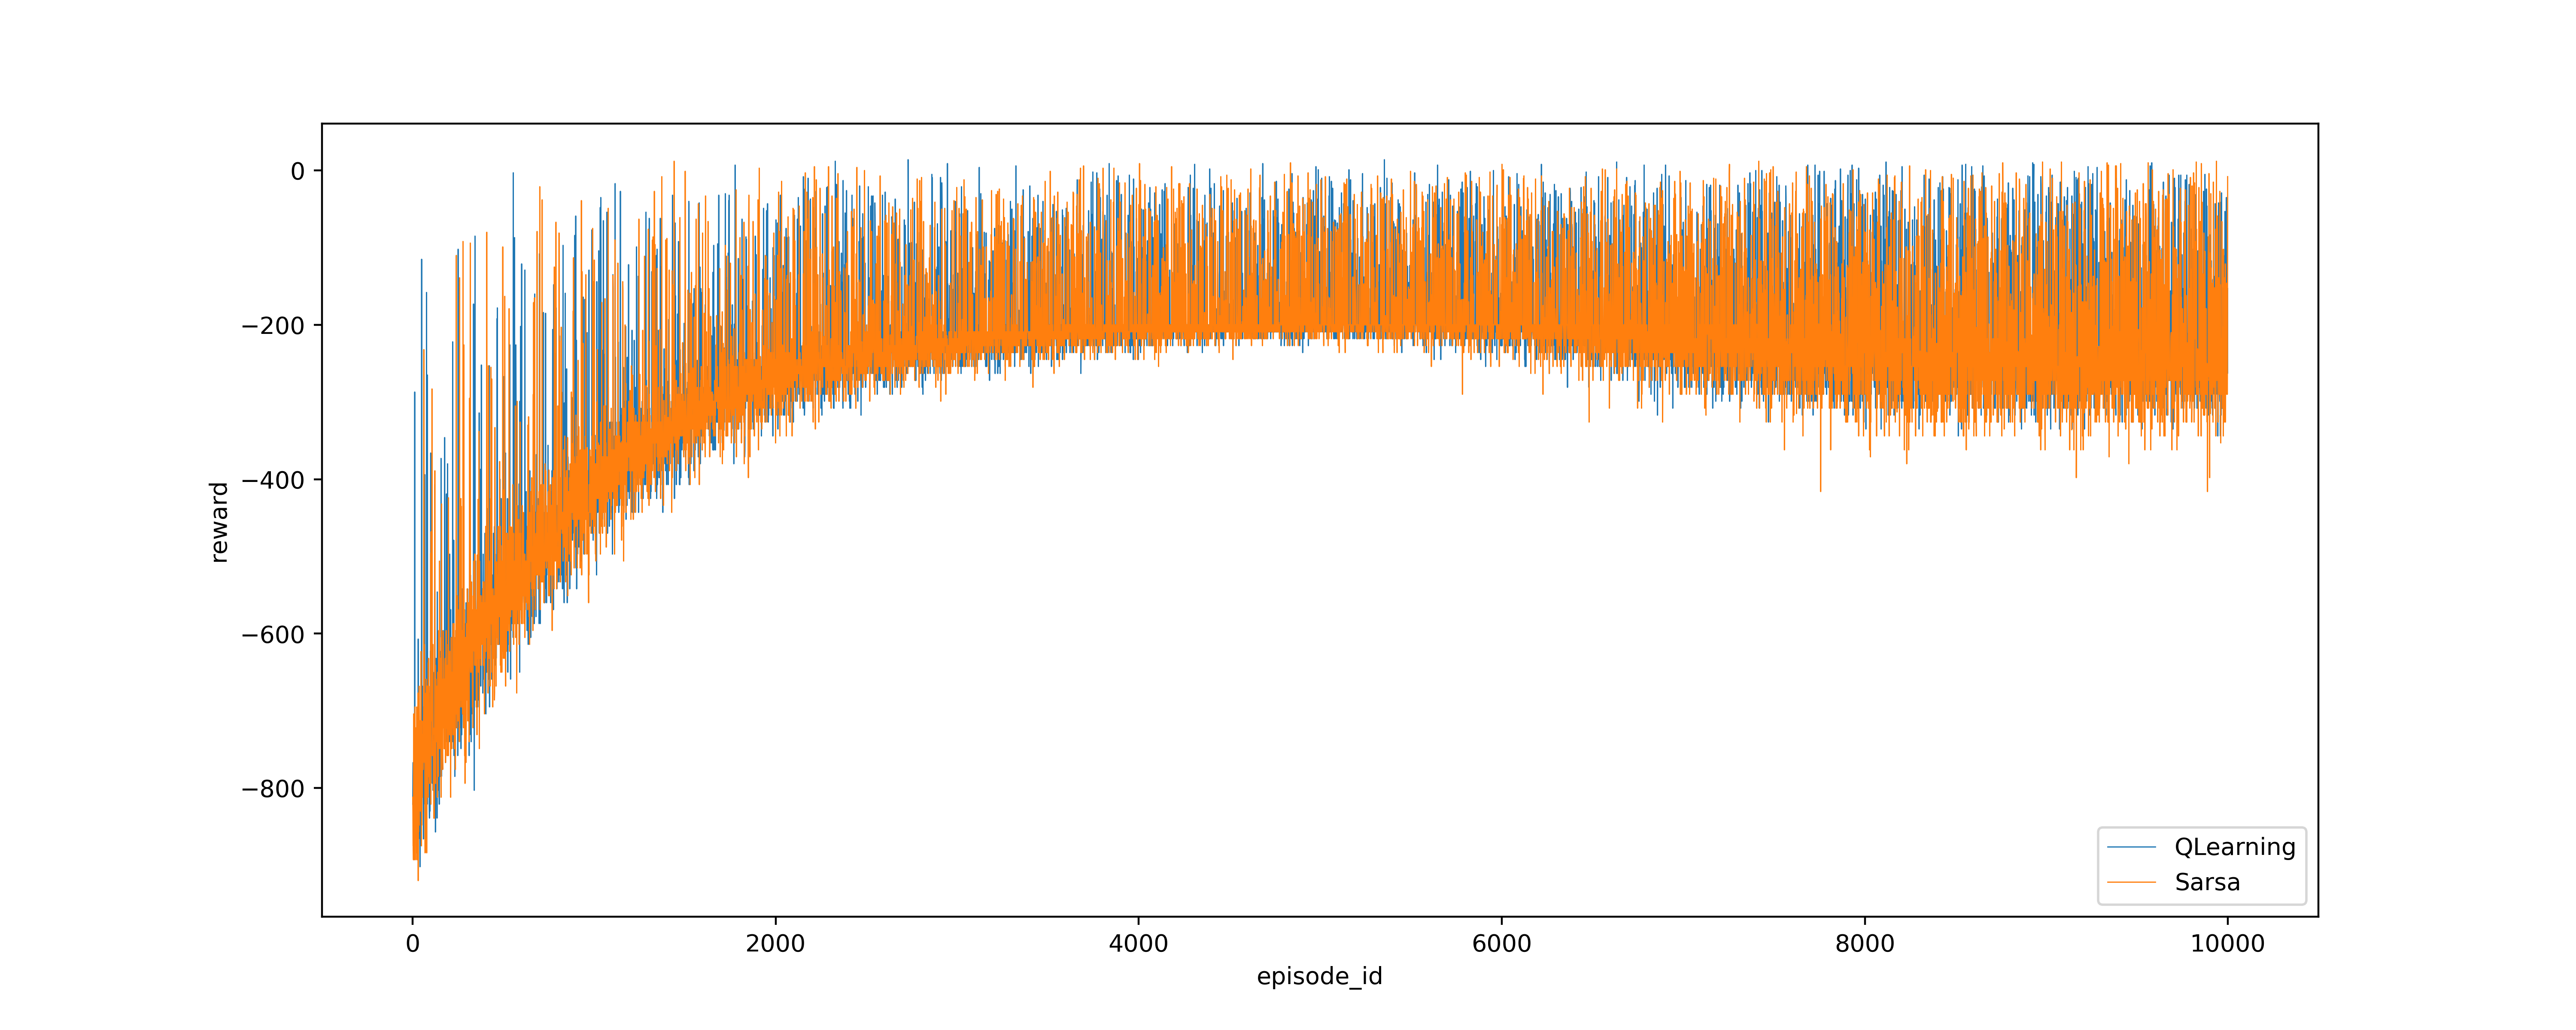
\includegraphics[width=1.00\columnwidth]{./assets/main(lr=0.0010).png}}
        \subfigure[lr = 0.005]{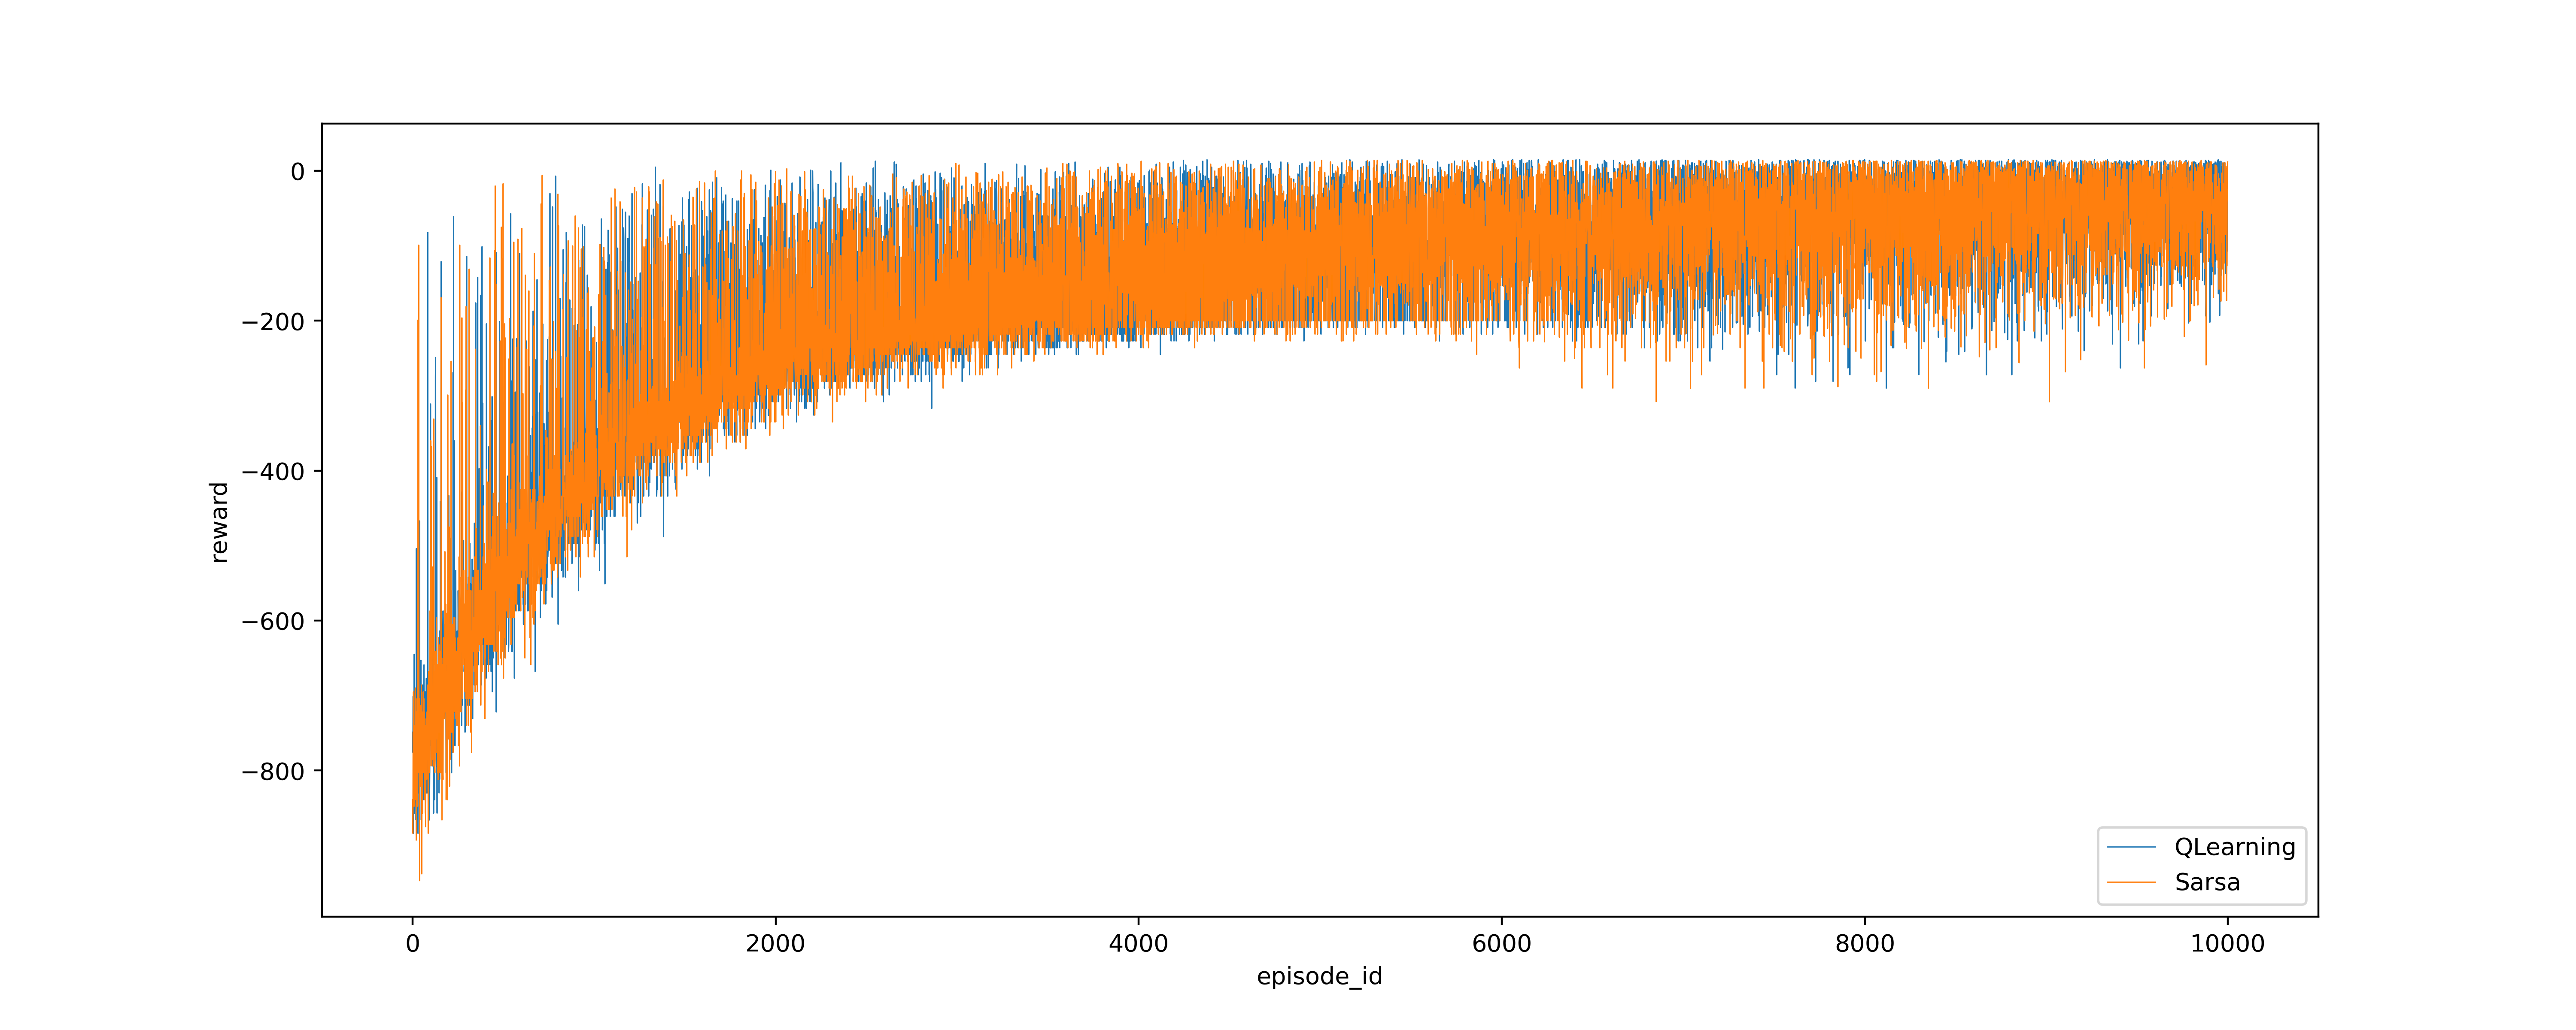
\includegraphics[width=1.00\columnwidth]{./assets/main(lr=0.0050).png}}
        \subfigure[lr = 0.01]{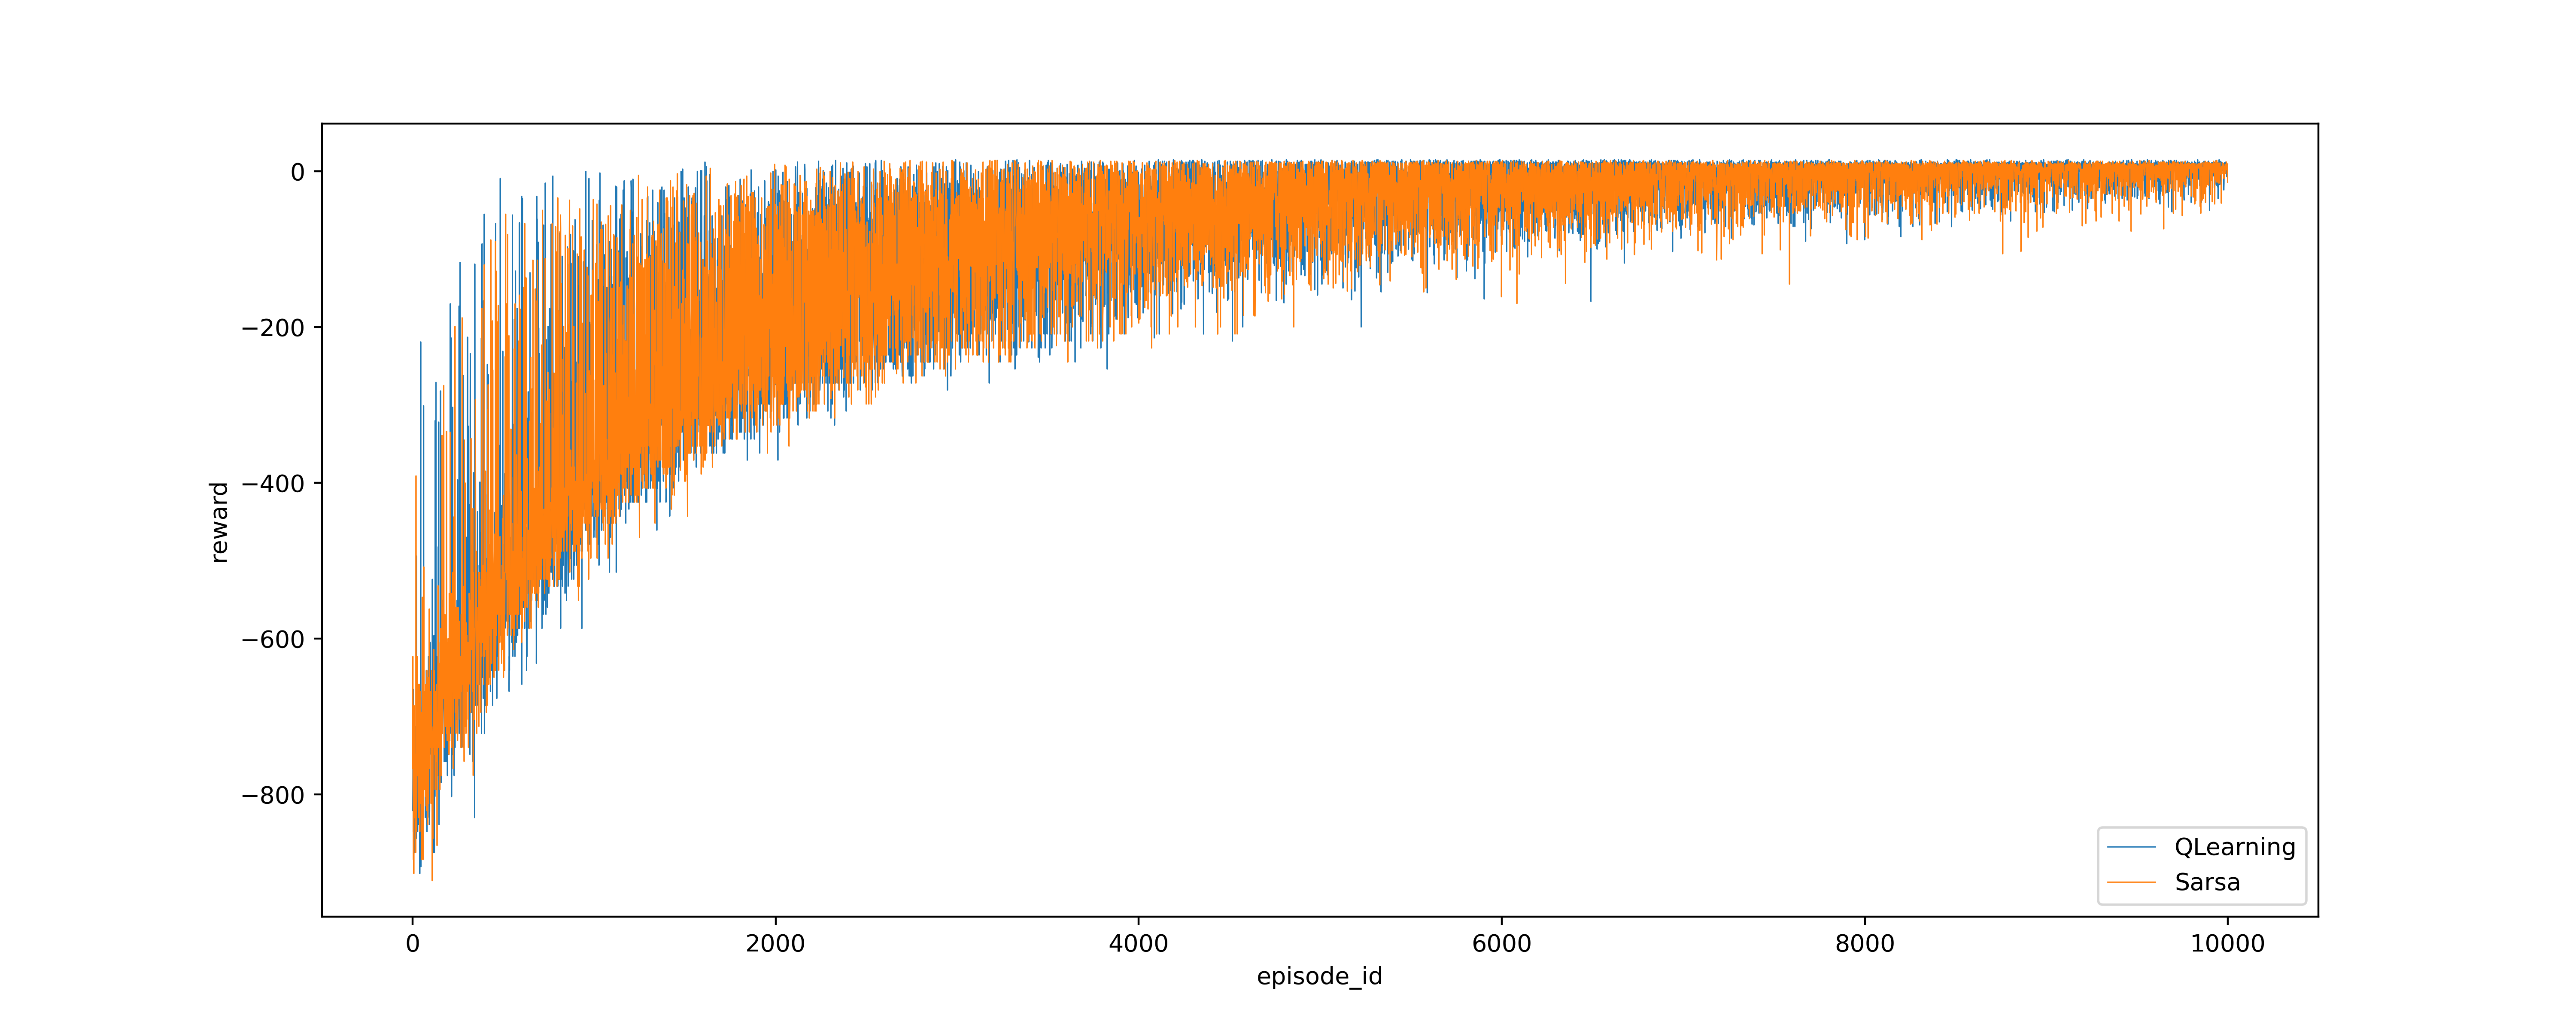
\includegraphics[width=1.00\columnwidth]{./assets/main(lr=0.0100).png}}
        \caption{QLearning和Sarsa算法在不同迭代步长下的奖励值变化情况(1)}
        \end{figure}

        \begin{figure}[htbp]
        \centering
        \subfigure[lr = 0.05]{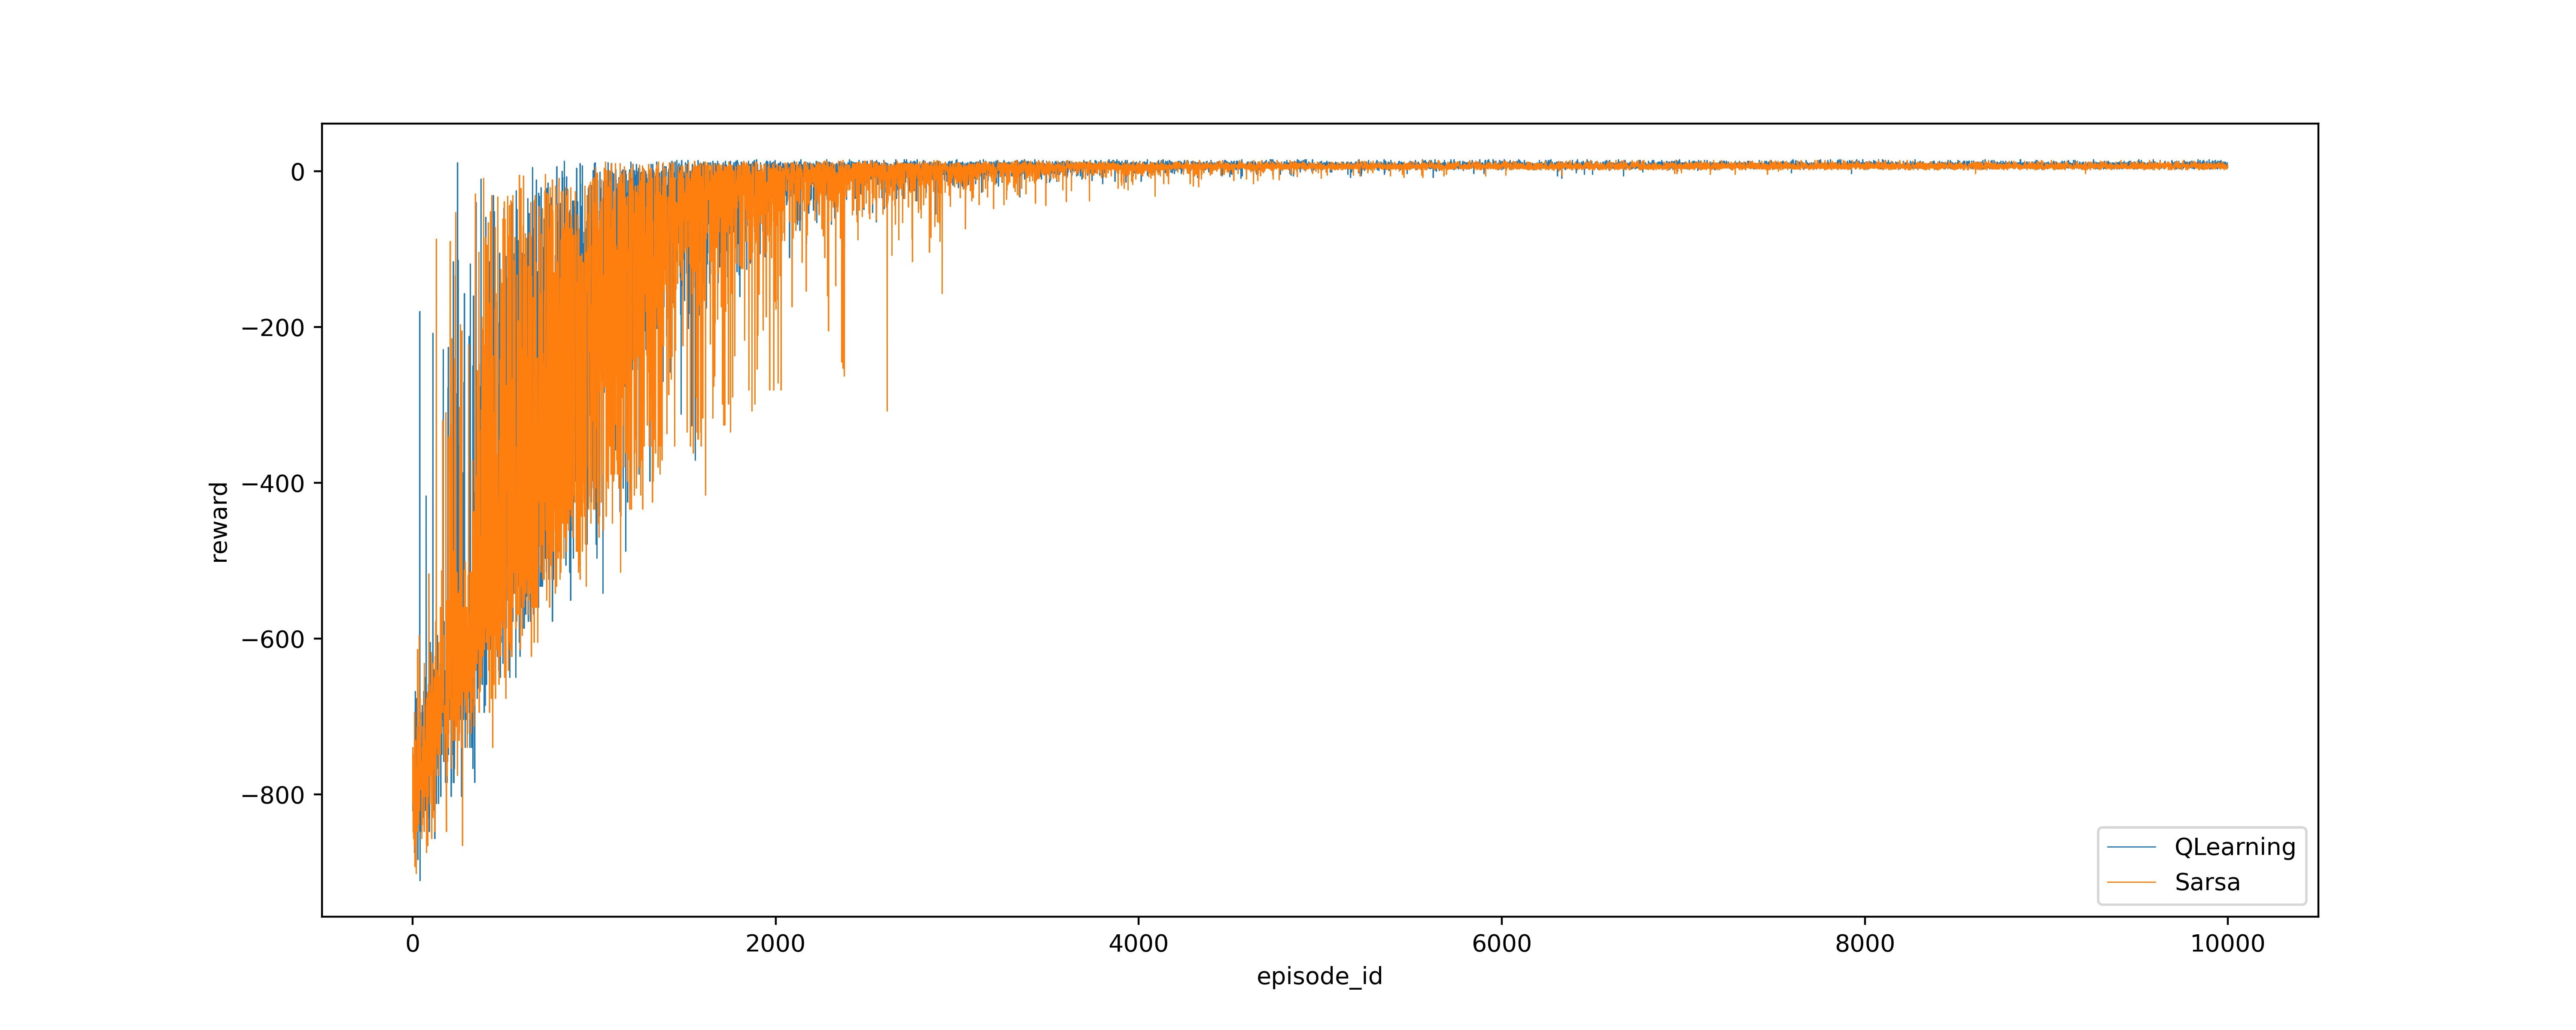
\includegraphics[width=1.00\columnwidth]{./assets/main(lr=0.0500).png}}
        \subfigure[lr = 0.1]{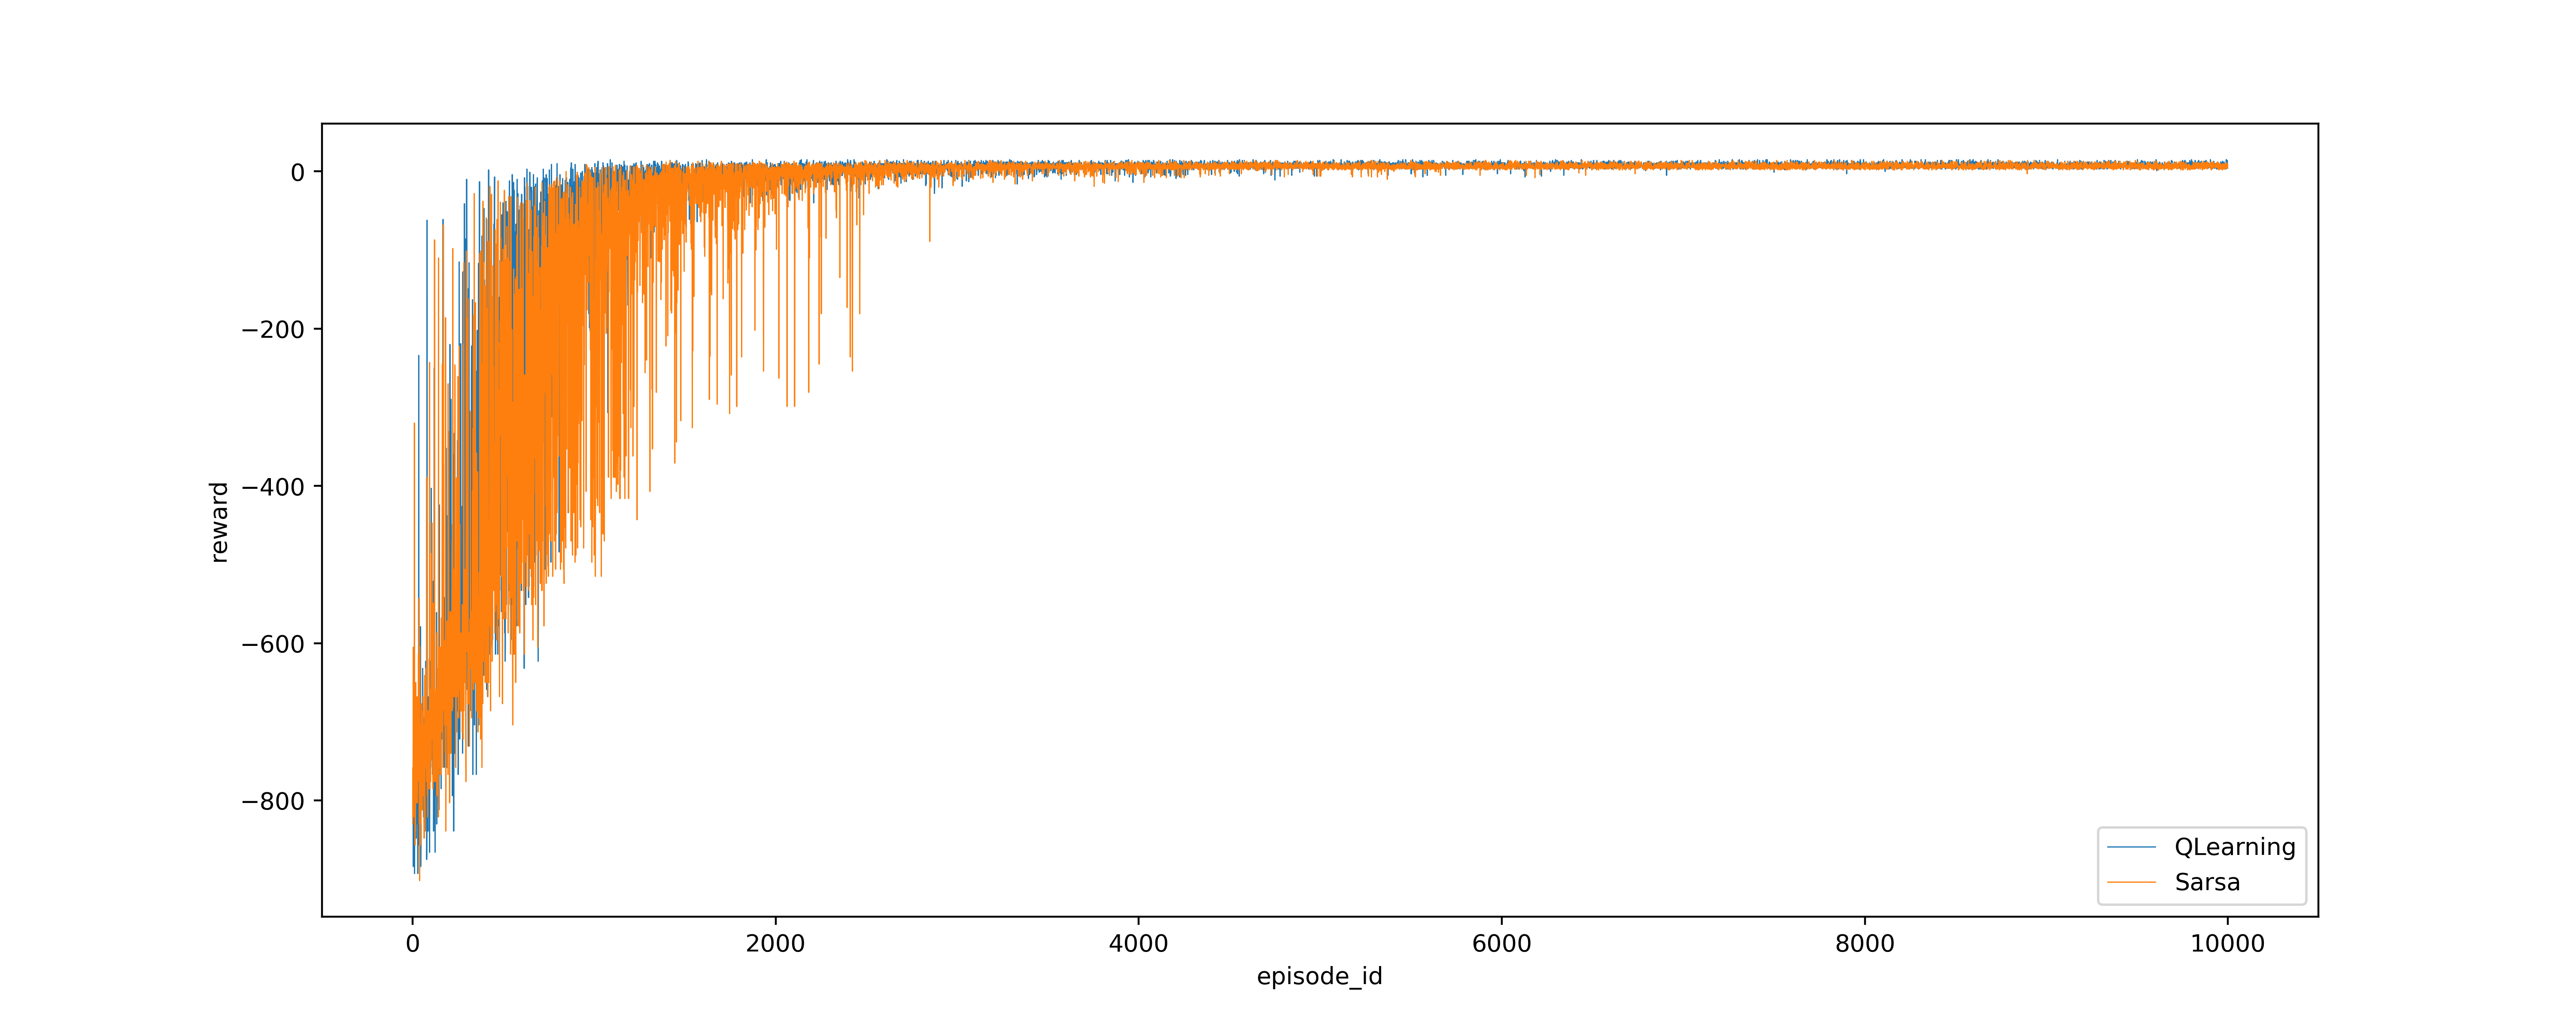
\includegraphics[width=1.00\columnwidth]{./assets/main(lr=0.1000).png}}
        \subfigure[lr = 0.5]{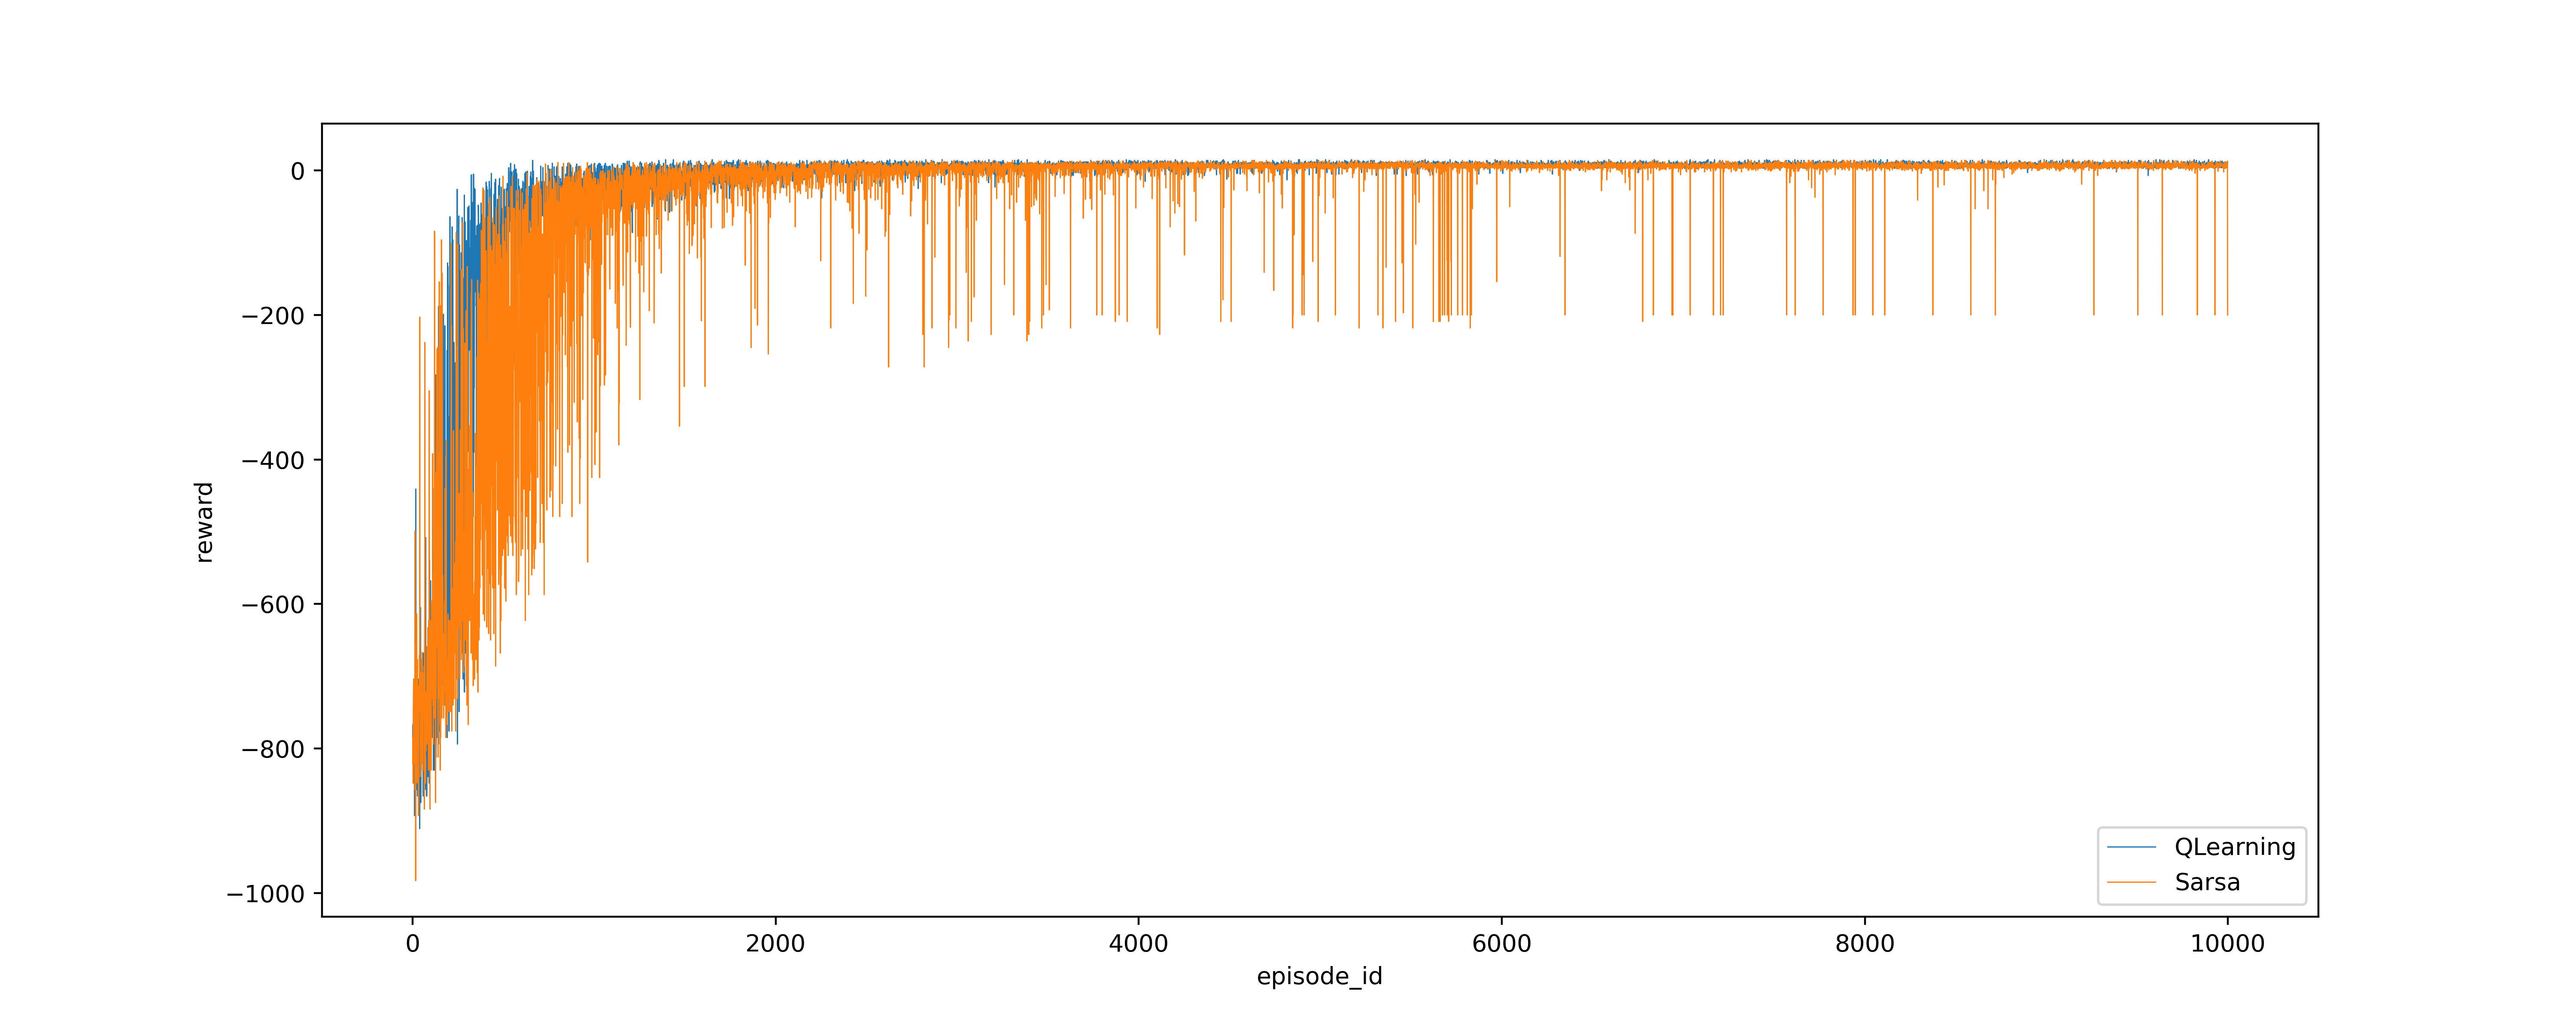
\includegraphics[width=1.00\columnwidth]{./assets/main(lr=0.5000).png}}
        \caption{QLearning和Sarsa算法在不同迭代步长下的奖励值变化情况(2)}
        \end{figure}

        \begin{figure}[htbp]
        \centering
        \subfigure[lr = 1]{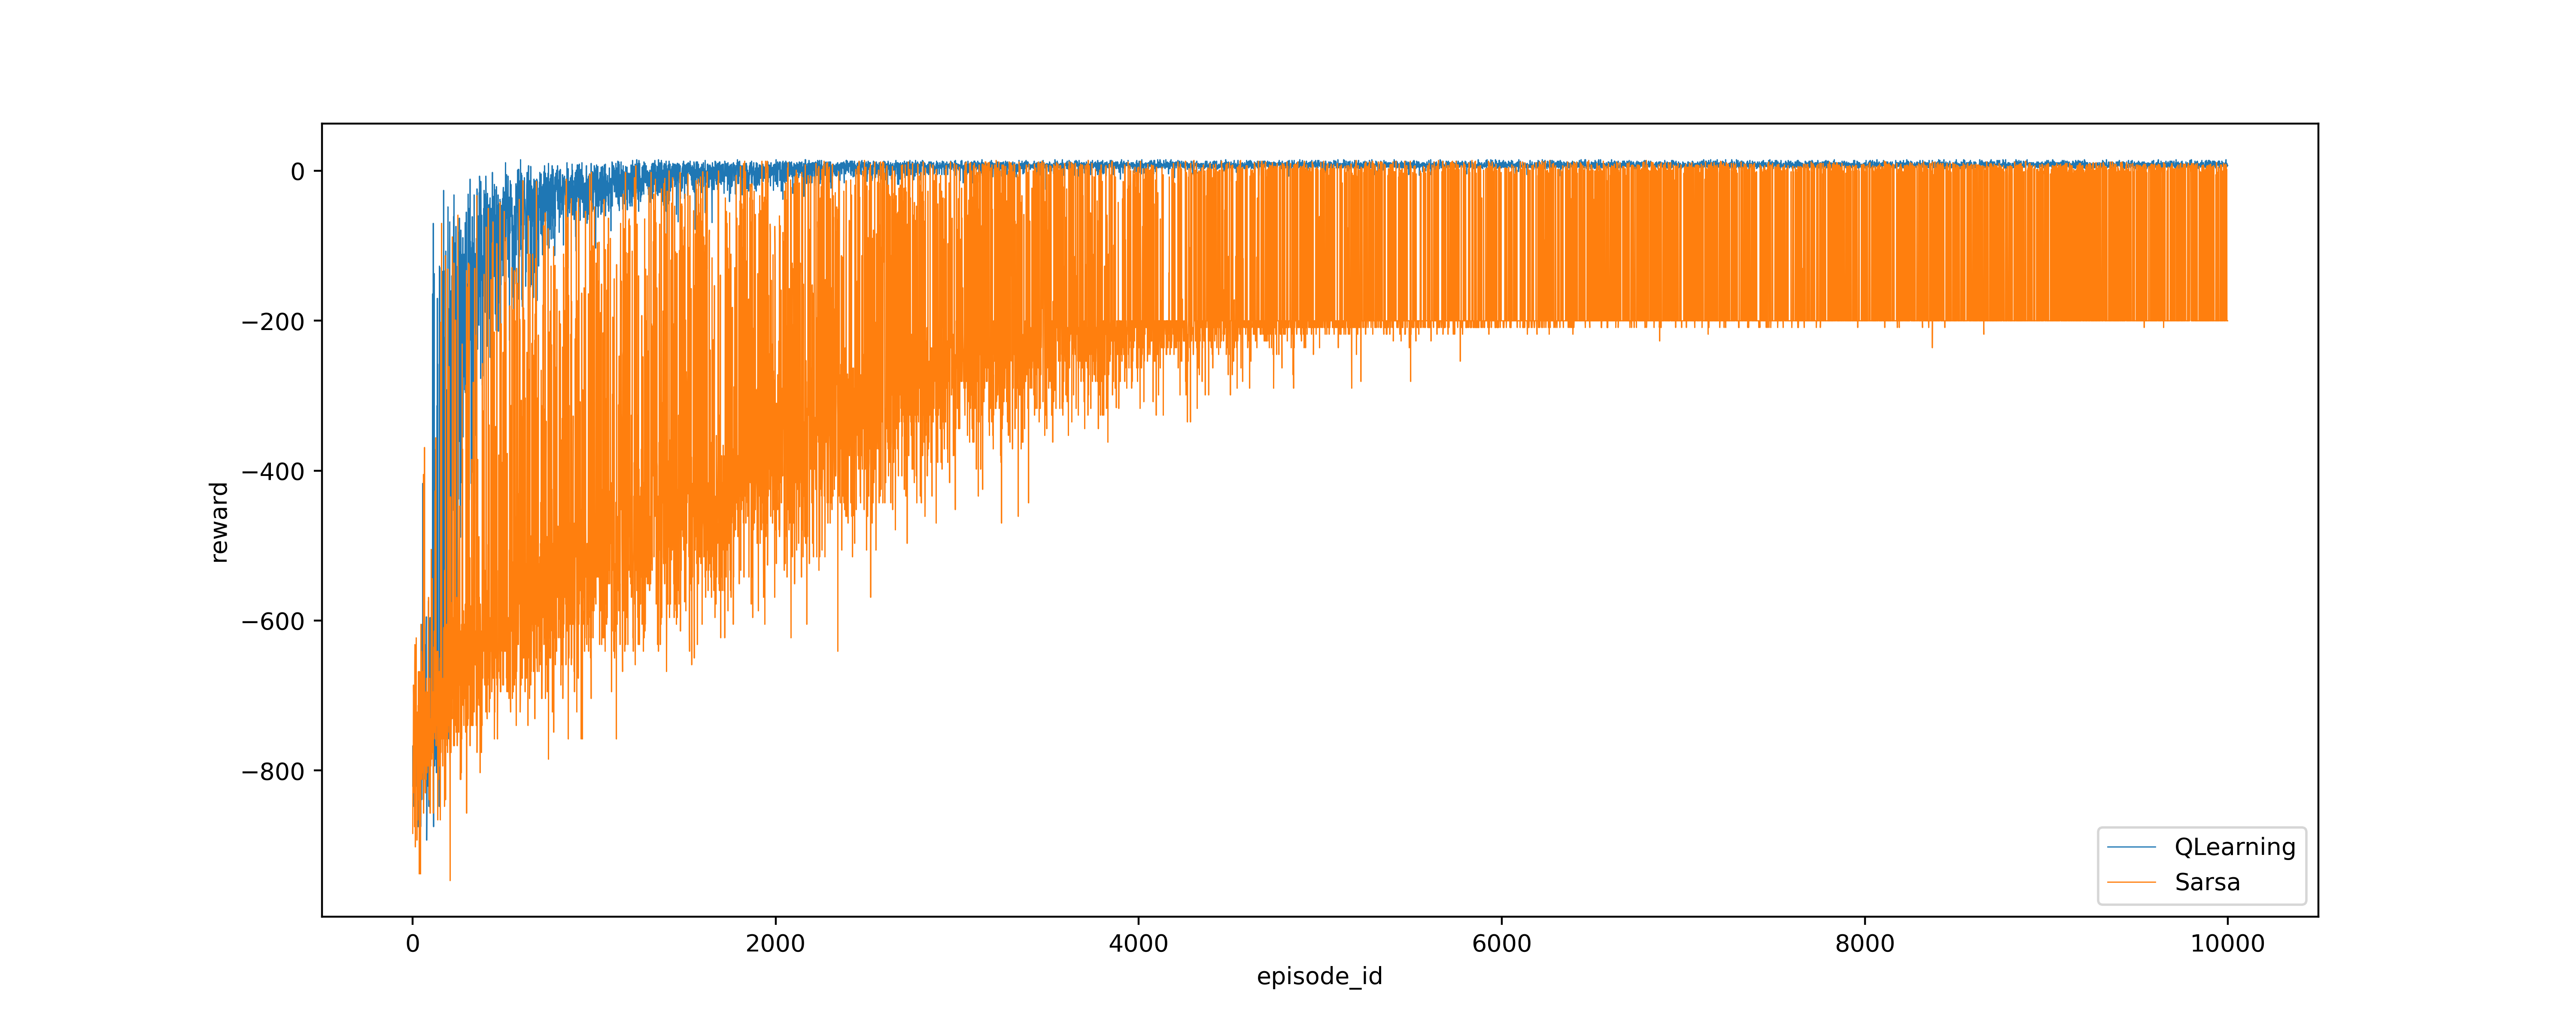
\includegraphics[width=1.00\columnwidth]{./assets/main(lr=1.0000).png}}
        \subfigure[lr = 5]{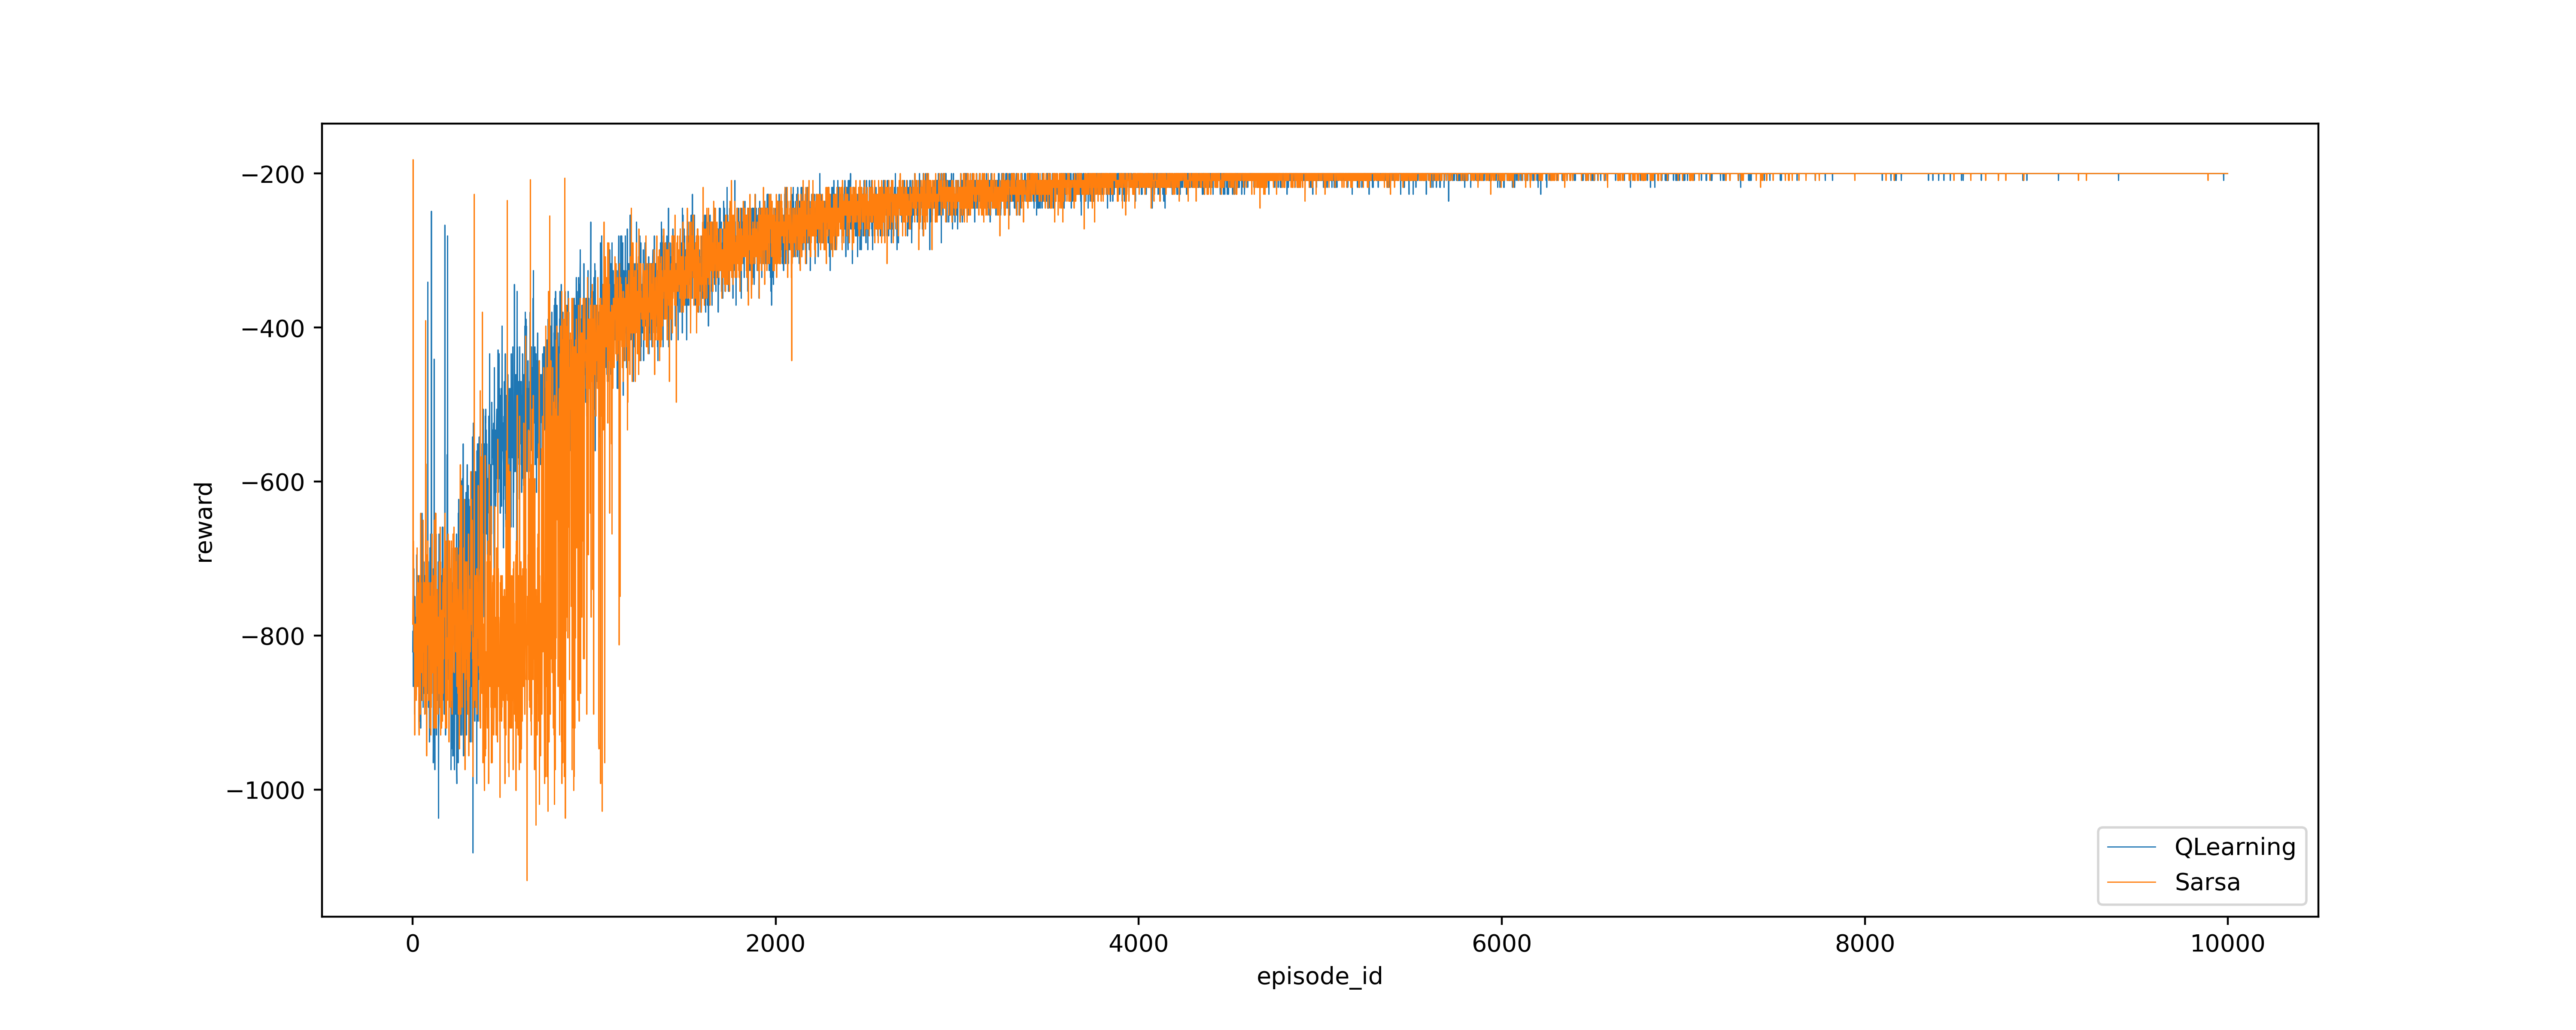
\includegraphics[width=1.00\columnwidth]{./assets/main(lr=5.0000).png}}
        \subfigure[lr = 10]{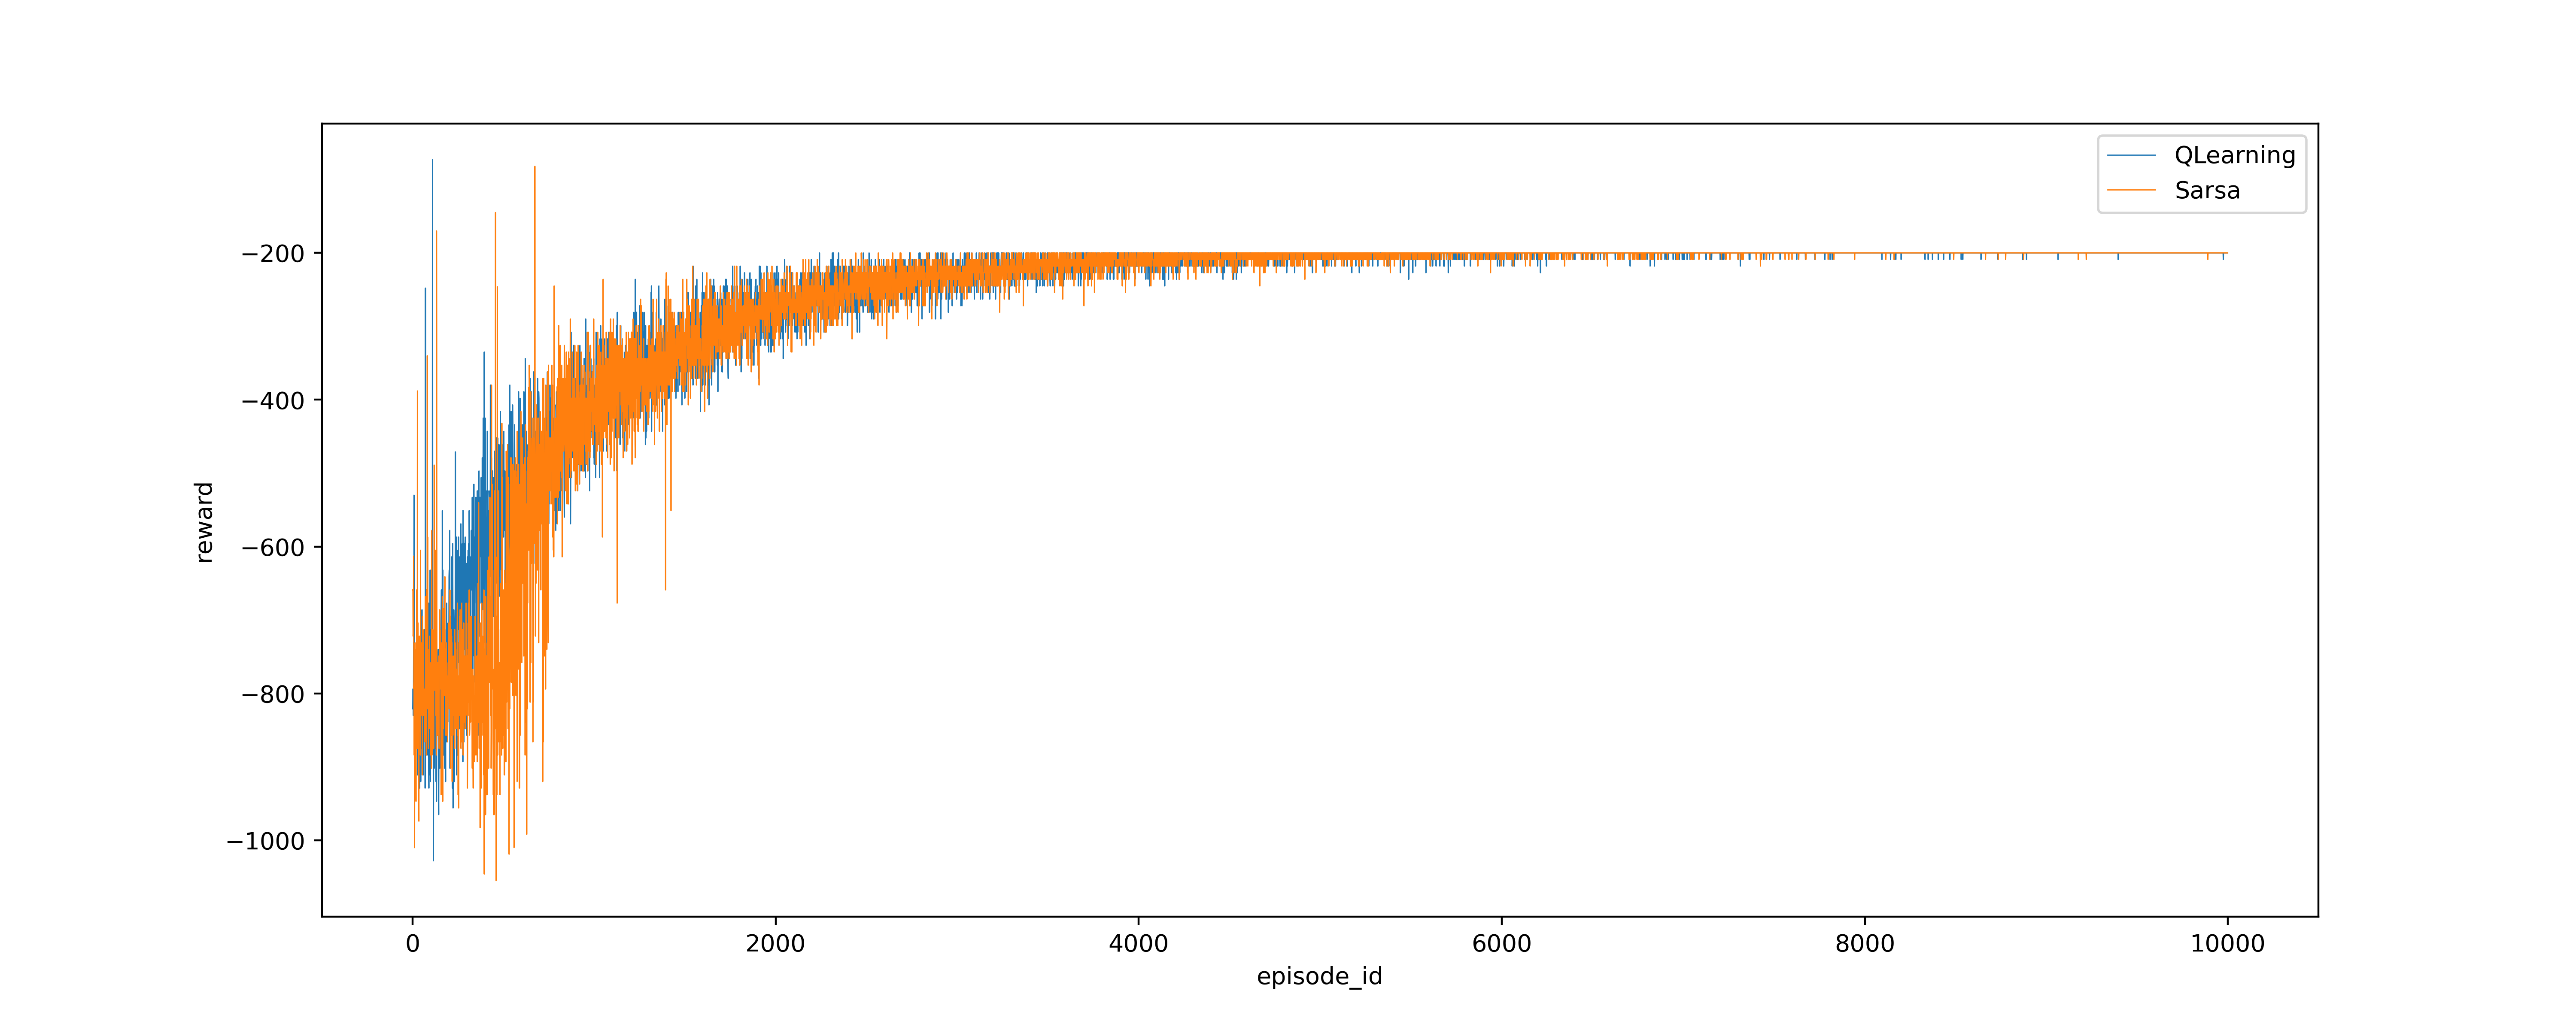
\includegraphics[width=1.00\columnwidth]{./assets/main(lr=10.0000).png}}
        \caption{QLearning和Sarsa算法在不同迭代步长下的奖励值变化情况(3)}
        \end{figure}

        \begin{table}[htbp]
        \caption{QLearning算法在不同迭代步长下的性能表现}
        \centering
        \begin{tabular}{cccc}
            \toprule
            lr    & 最终奖励值 & 平均所需步数 & 迭代稳定性 \\
            \midrule
            0.001 &  -406.42  &   [Fail]    &     差     \\
            0.005 &  -233.48  &   181.79    &     差     \\
            0.010 &  -99.410  &   109.49    &     差     \\
            0.050 &   8.045   &   12.955    &     良好   \\
            0.100 &   8.035   &   12.965    &     良好   \\
            0.500 &   8.090   &   12.910    &     良好   \\
            1.000 &   7.765   &   13.235    &     良好   \\
            5.000 &  -200.00  &   [Fail]    &     良好（收敛到了较差的策略）\\
            10.00 &  -200.00  &   [Fail]    &     良好（收敛到了较差的策略）\\
        \end{tabular}
        \end{table}

        \begin{table}[htbp]
        \caption{Sarsa算法在不同迭代步长下的性能表现}
        \centering
        \begin{tabular}{cccc}
            \toprule
            lr    & 最终奖励值 & 平均所需步数 & 迭代稳定性 \\
            \midrule
            0.001 &  -478.28  &   [Fail]    &    差      \\
            0.005 &  -223.21  &   172.30    &    差      \\
            0.010 &  -148.06  &   104.93    &    差      \\
            0.050 &   7.540   &   13.460    &    良好    \\
            0.100 &   7.280   &   13.720    &    良好    \\
            0.500 &   7.265   &   13.735    &    中等    \\
            1.000 &  -149.64  &   154.68    &    差      \\
            5.000 &  -200.00  &   [Fail]    &    良好（收敛到了较差的策略）\\
            10.00 &  -200.00  &   [Fail]    &    良好（收敛到了较差的策略）\\
        \end{tabular}
        \end{table}

        固定随机数种子为42，分别取迭代步长为0.001，0.005，0.01，0.05，0.1，0.5，1，5，10，进行训练和测试。
        在训练过程中，QLearning和Sarsa算法在不同迭代步长下的奖励值变化情况如图1，图2，图3所示。

        在测试中，QLearning和Sarsa算法在不同迭代步长下的最终奖励值、完成任务所需的平均步数和算法迭代稳定性情况如表1、表2所示。

        可以看出，QLearning和Sarsa算法均对迭代步长有较高的要求，在小于0.05或大于0.5的迭代步长下均无法学习到较好的策略。

        在迭代步长等于0.5时，QLearning算法能够取得最好的效果，
        获得的最终奖励值为8.090（最大），完成任务所需的平均步数为12.910（最少），收敛情况稳定（在2000个episode后收敛）。

        在迭代步长等于0.05时，Sarsa算法能够取得最好的效果，
        获得的最终奖励值为7.540（最大），完成任务所需的平均步数为13.460（最少），收敛情况稳定（在3000个episode后收敛）。

    \item 对比QLearning算法和Sarsa算法的实验效果。

        横向对比，我们发现QLearning算法的效果更好，与我们在课堂上学习到的结论一致。

        从迭代稳定稳定性方面考量，从图1、图2、图3中可以看出，QLearning算法的收敛速度更快，
        且在更大的迭代步长区间内可以成功学习到较好的策略。
        这说明QLearning算法的鲁棒性更好。

        从学习能力方面考量，从表1、表2中可以看出，QLearning算法可获得的最大奖励值为8.090，大于Sarsa算法可获得的最大奖励值7.540。
        QLearning算法可获得的最小平均所需步数为12.910，亦小于Sarsa算法可获得的最小平均所需步数13.460。
        这说明QLearning算法可以学习到更优秀的策略。

    \end{enumerate}

\section{REINFORCE and AC}

    \begin{enumerate}

    \item 补全REINFORCE的代码。

        代码已补全，源代码参见./code/policy\_gradient/policy\_gradient.py中的REINFORCE类。

    \item 补全TDActorCritic的代码。

        代码已补全，源代码参见./code/policy\_gradient/policy\_gradient.py中的TDActorCritic类。

    \item 模型测试。

        分别选取随机数种子为0，21和42，将REINFORCE模型和TDActorCritic模型放在cartpole-v0和cartpole-v1环境中训练，
        并记录训练过程中的获得的奖励值与损失值。

        我们将两模型在两环境训练中的损失值与奖励值的变化情况绘制为折线图，如图4、图5、图6所示。

        \begin{figure}[htbp]
        \centering
        \subfigure[REINFORCE, seed=0]{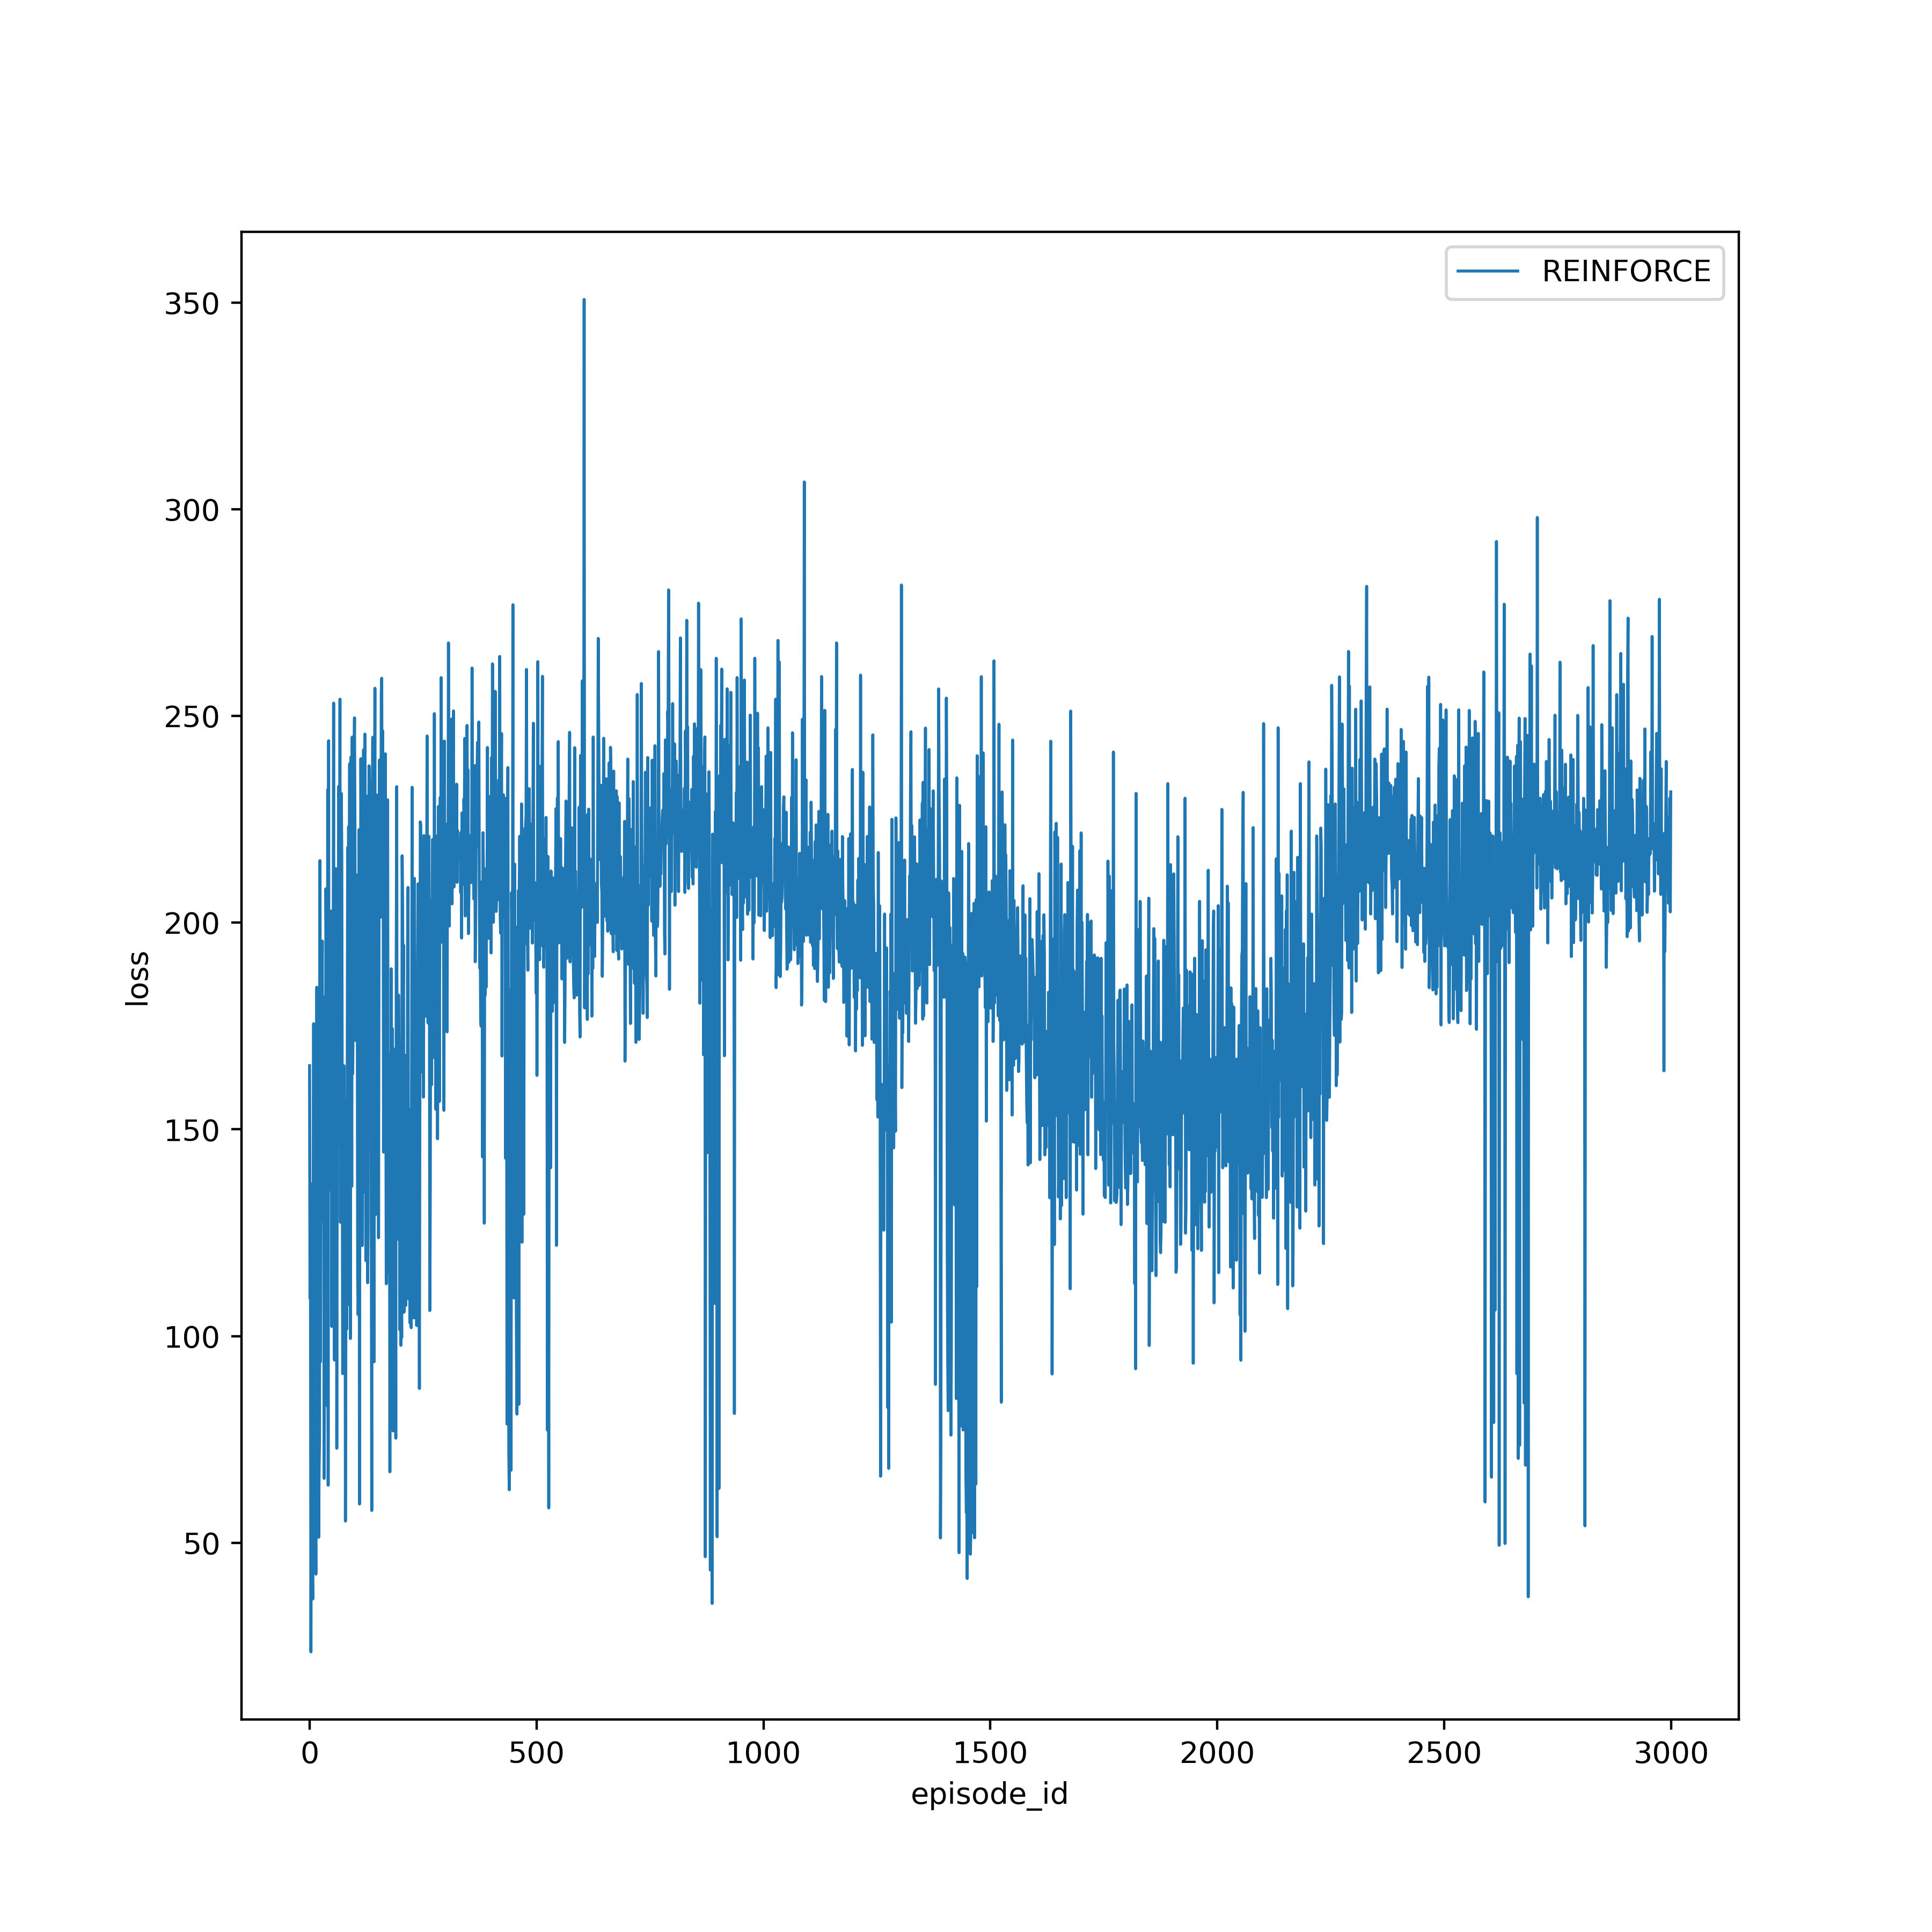
\includegraphics[width=0.40\columnwidth]{./assets/loss_REINFORCE (0, v0).png}}
        \subfigure[TDActorCritic, seed=0]{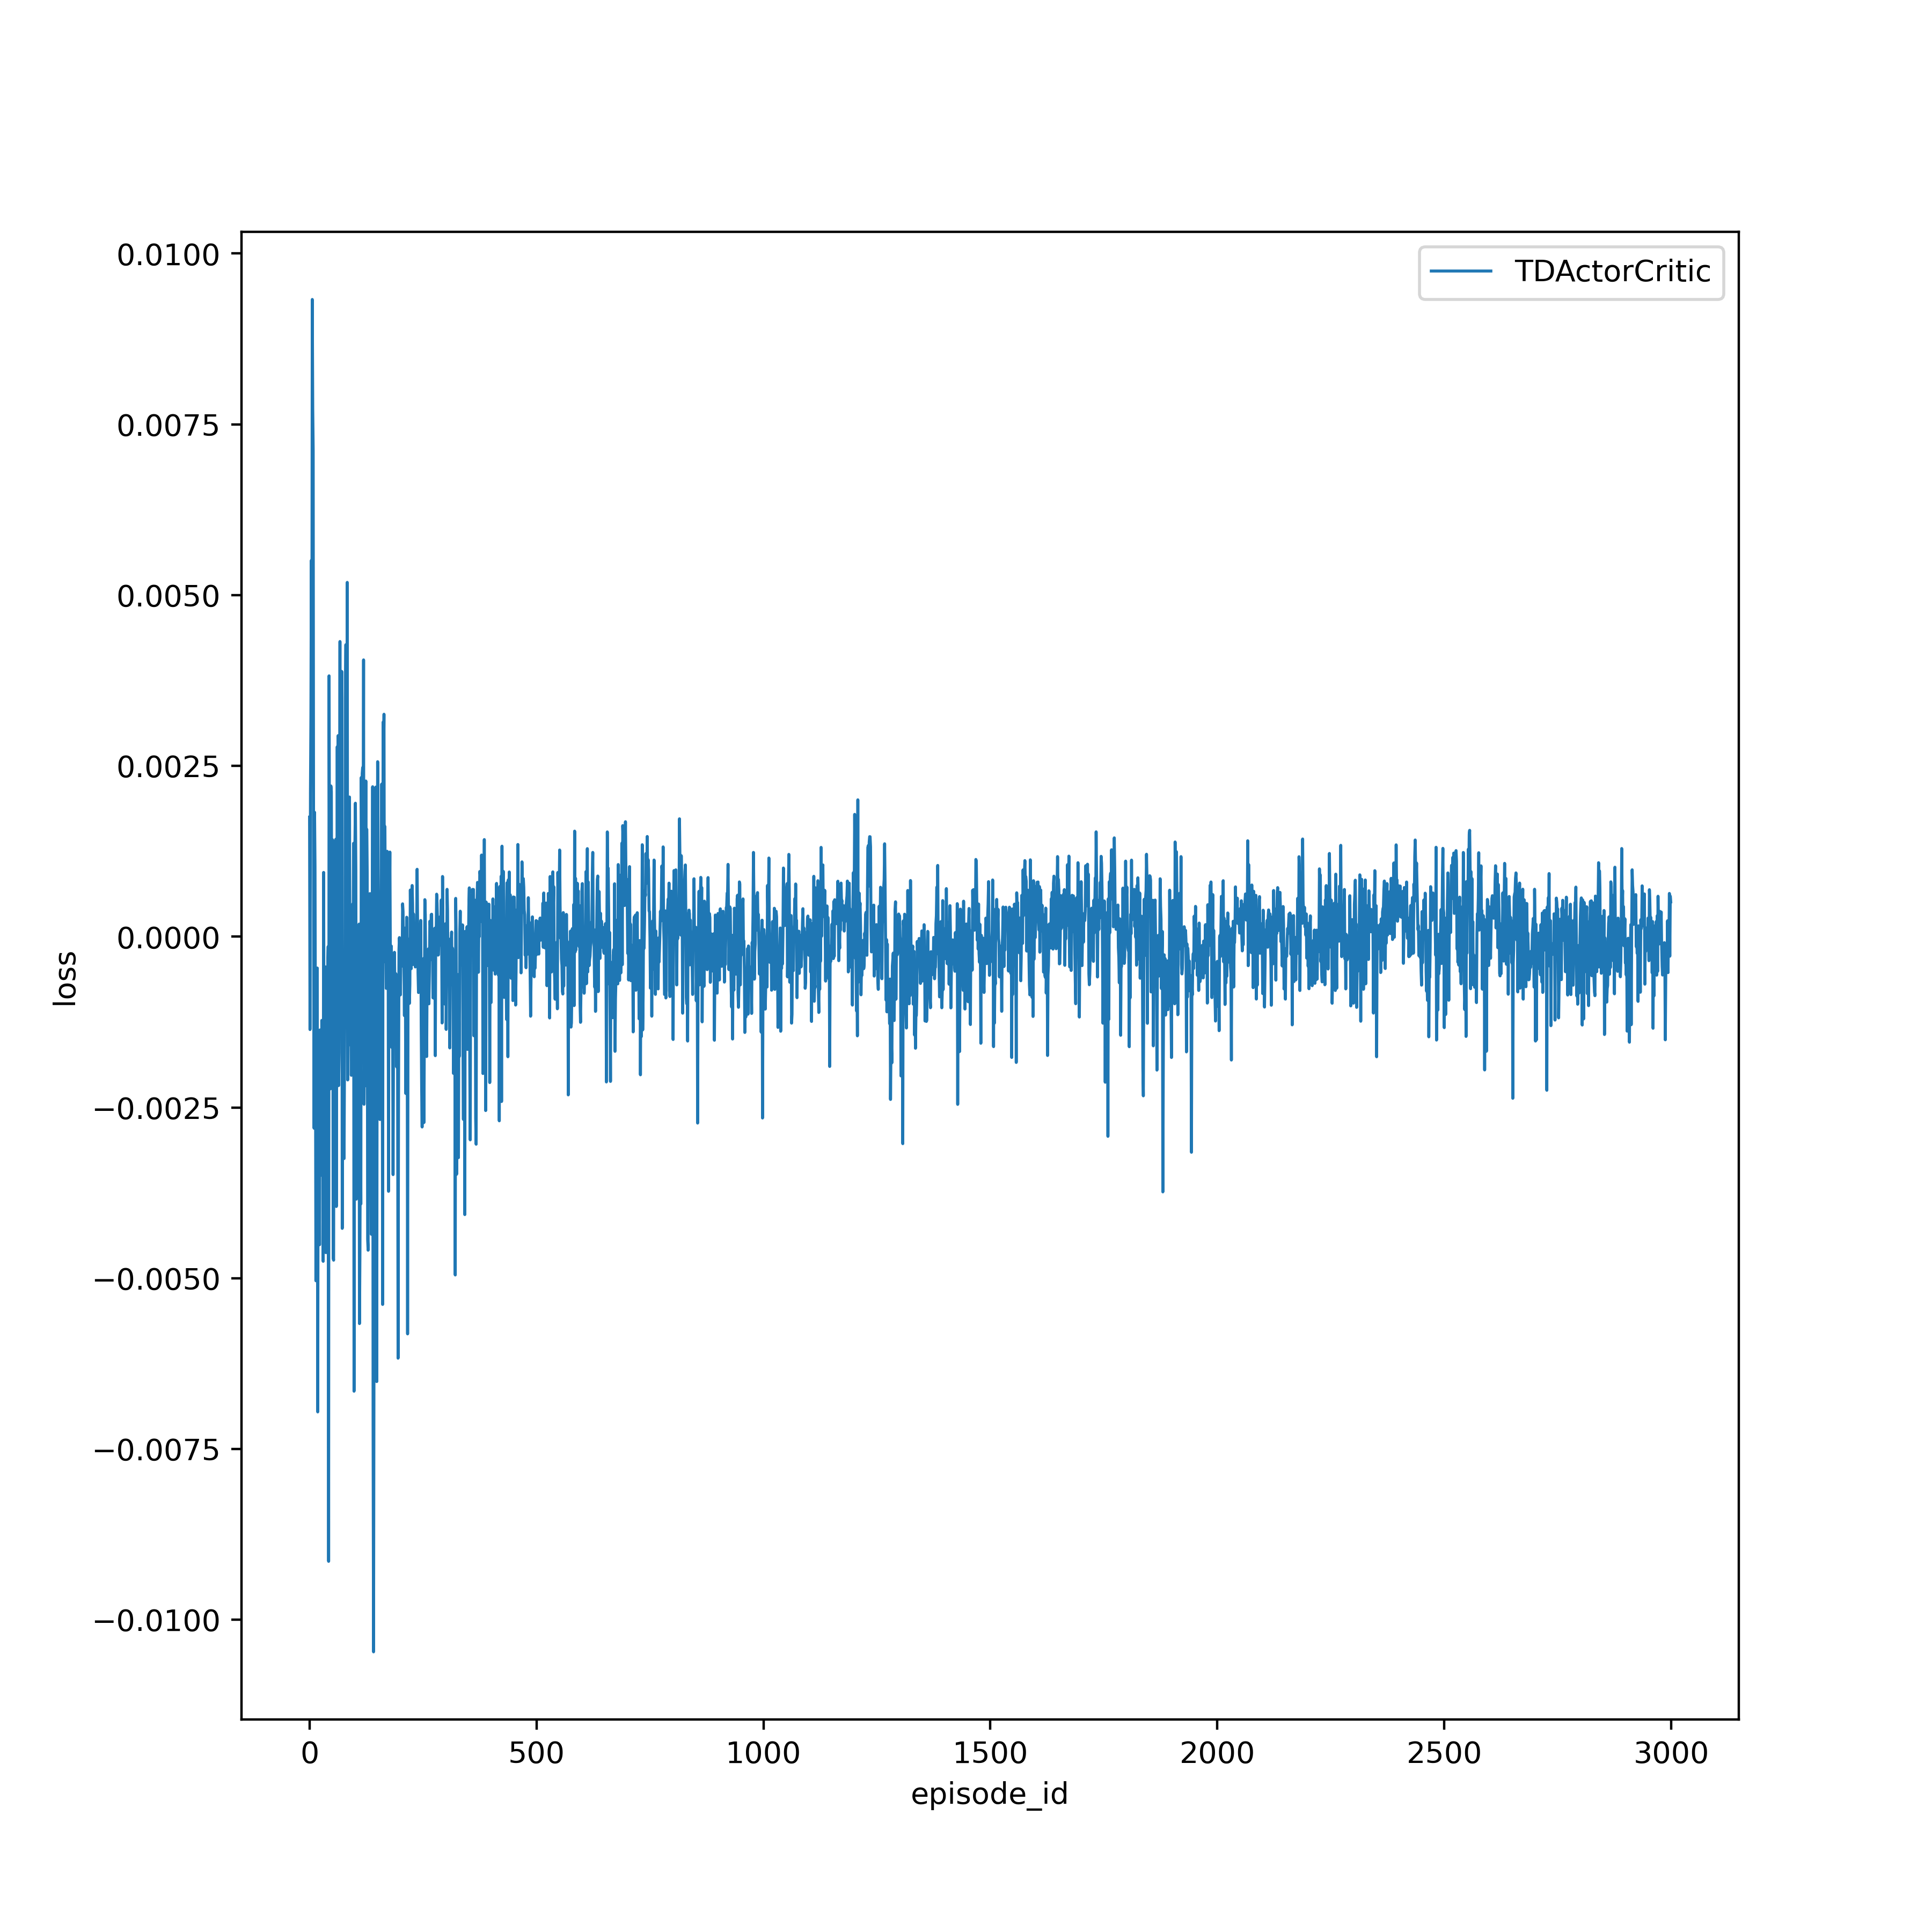
\includegraphics[width=0.40\columnwidth]{./assets/loss_TDAC (0, v0).png}}
        \subfigure[REINFORCE, seed=21]{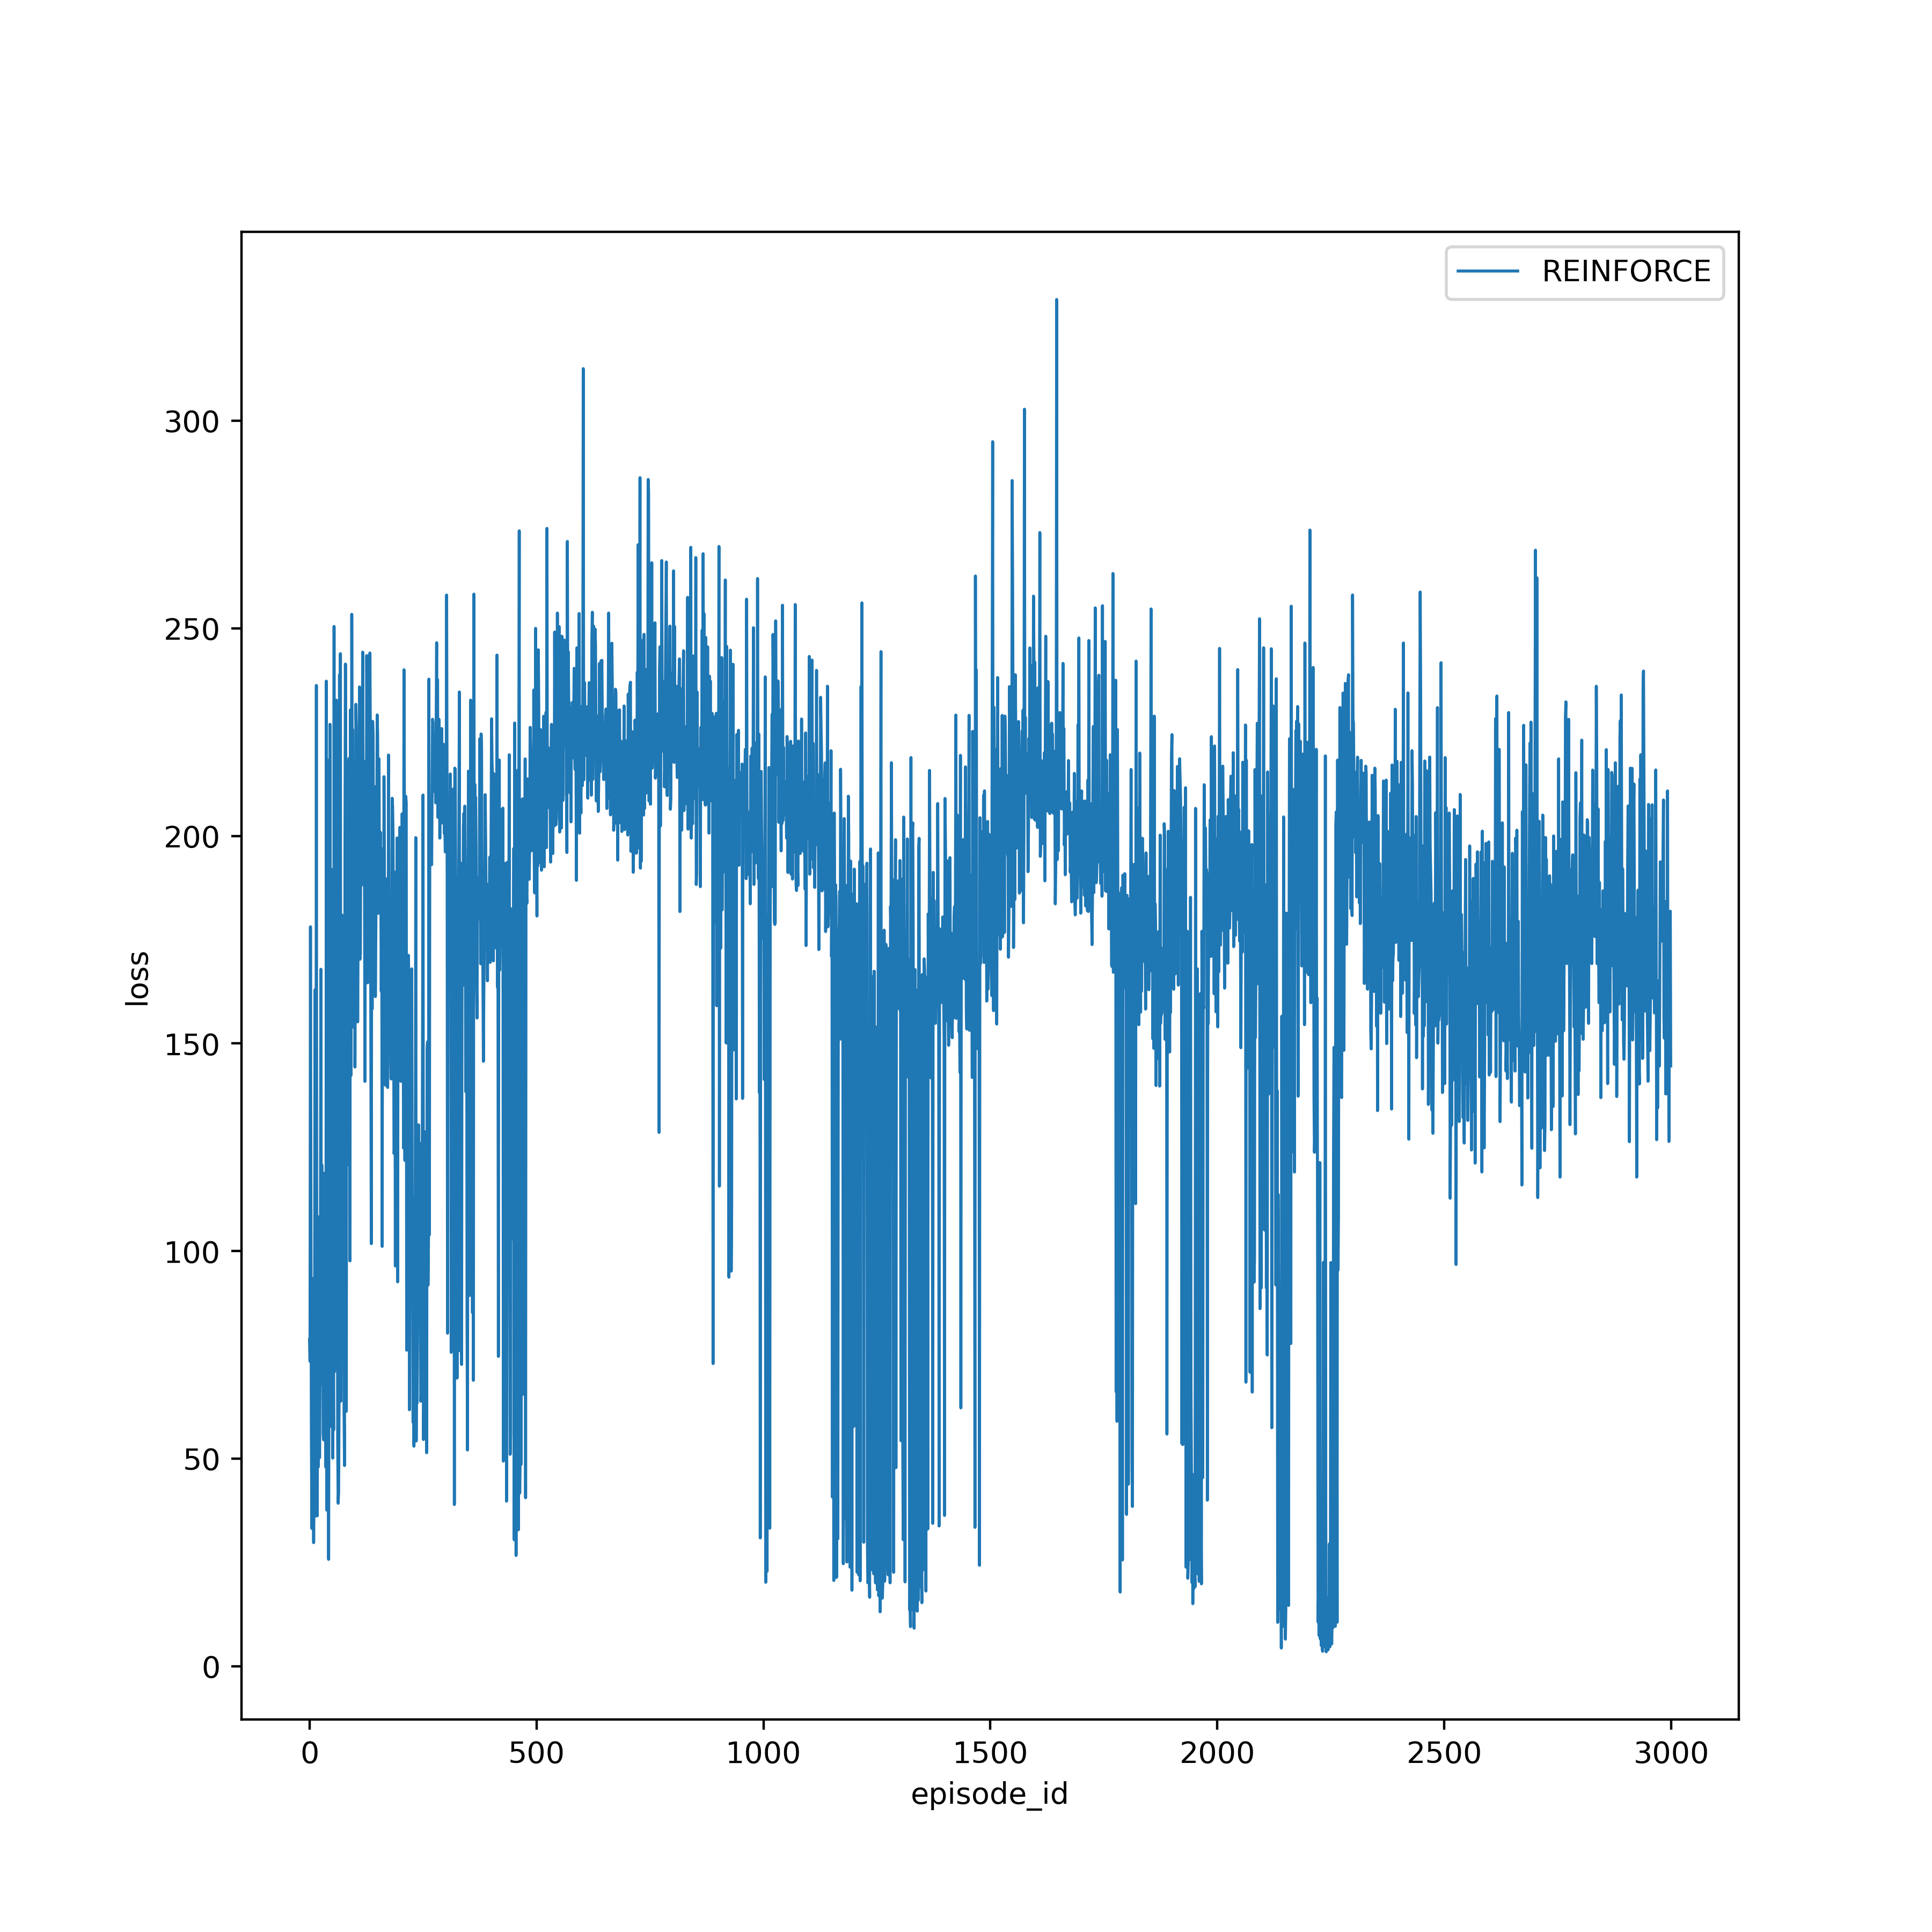
\includegraphics[width=0.40\columnwidth]{./assets/loss_REINFORCE (21, v0).png}}
        \subfigure[TDActorCritic, seed=21]{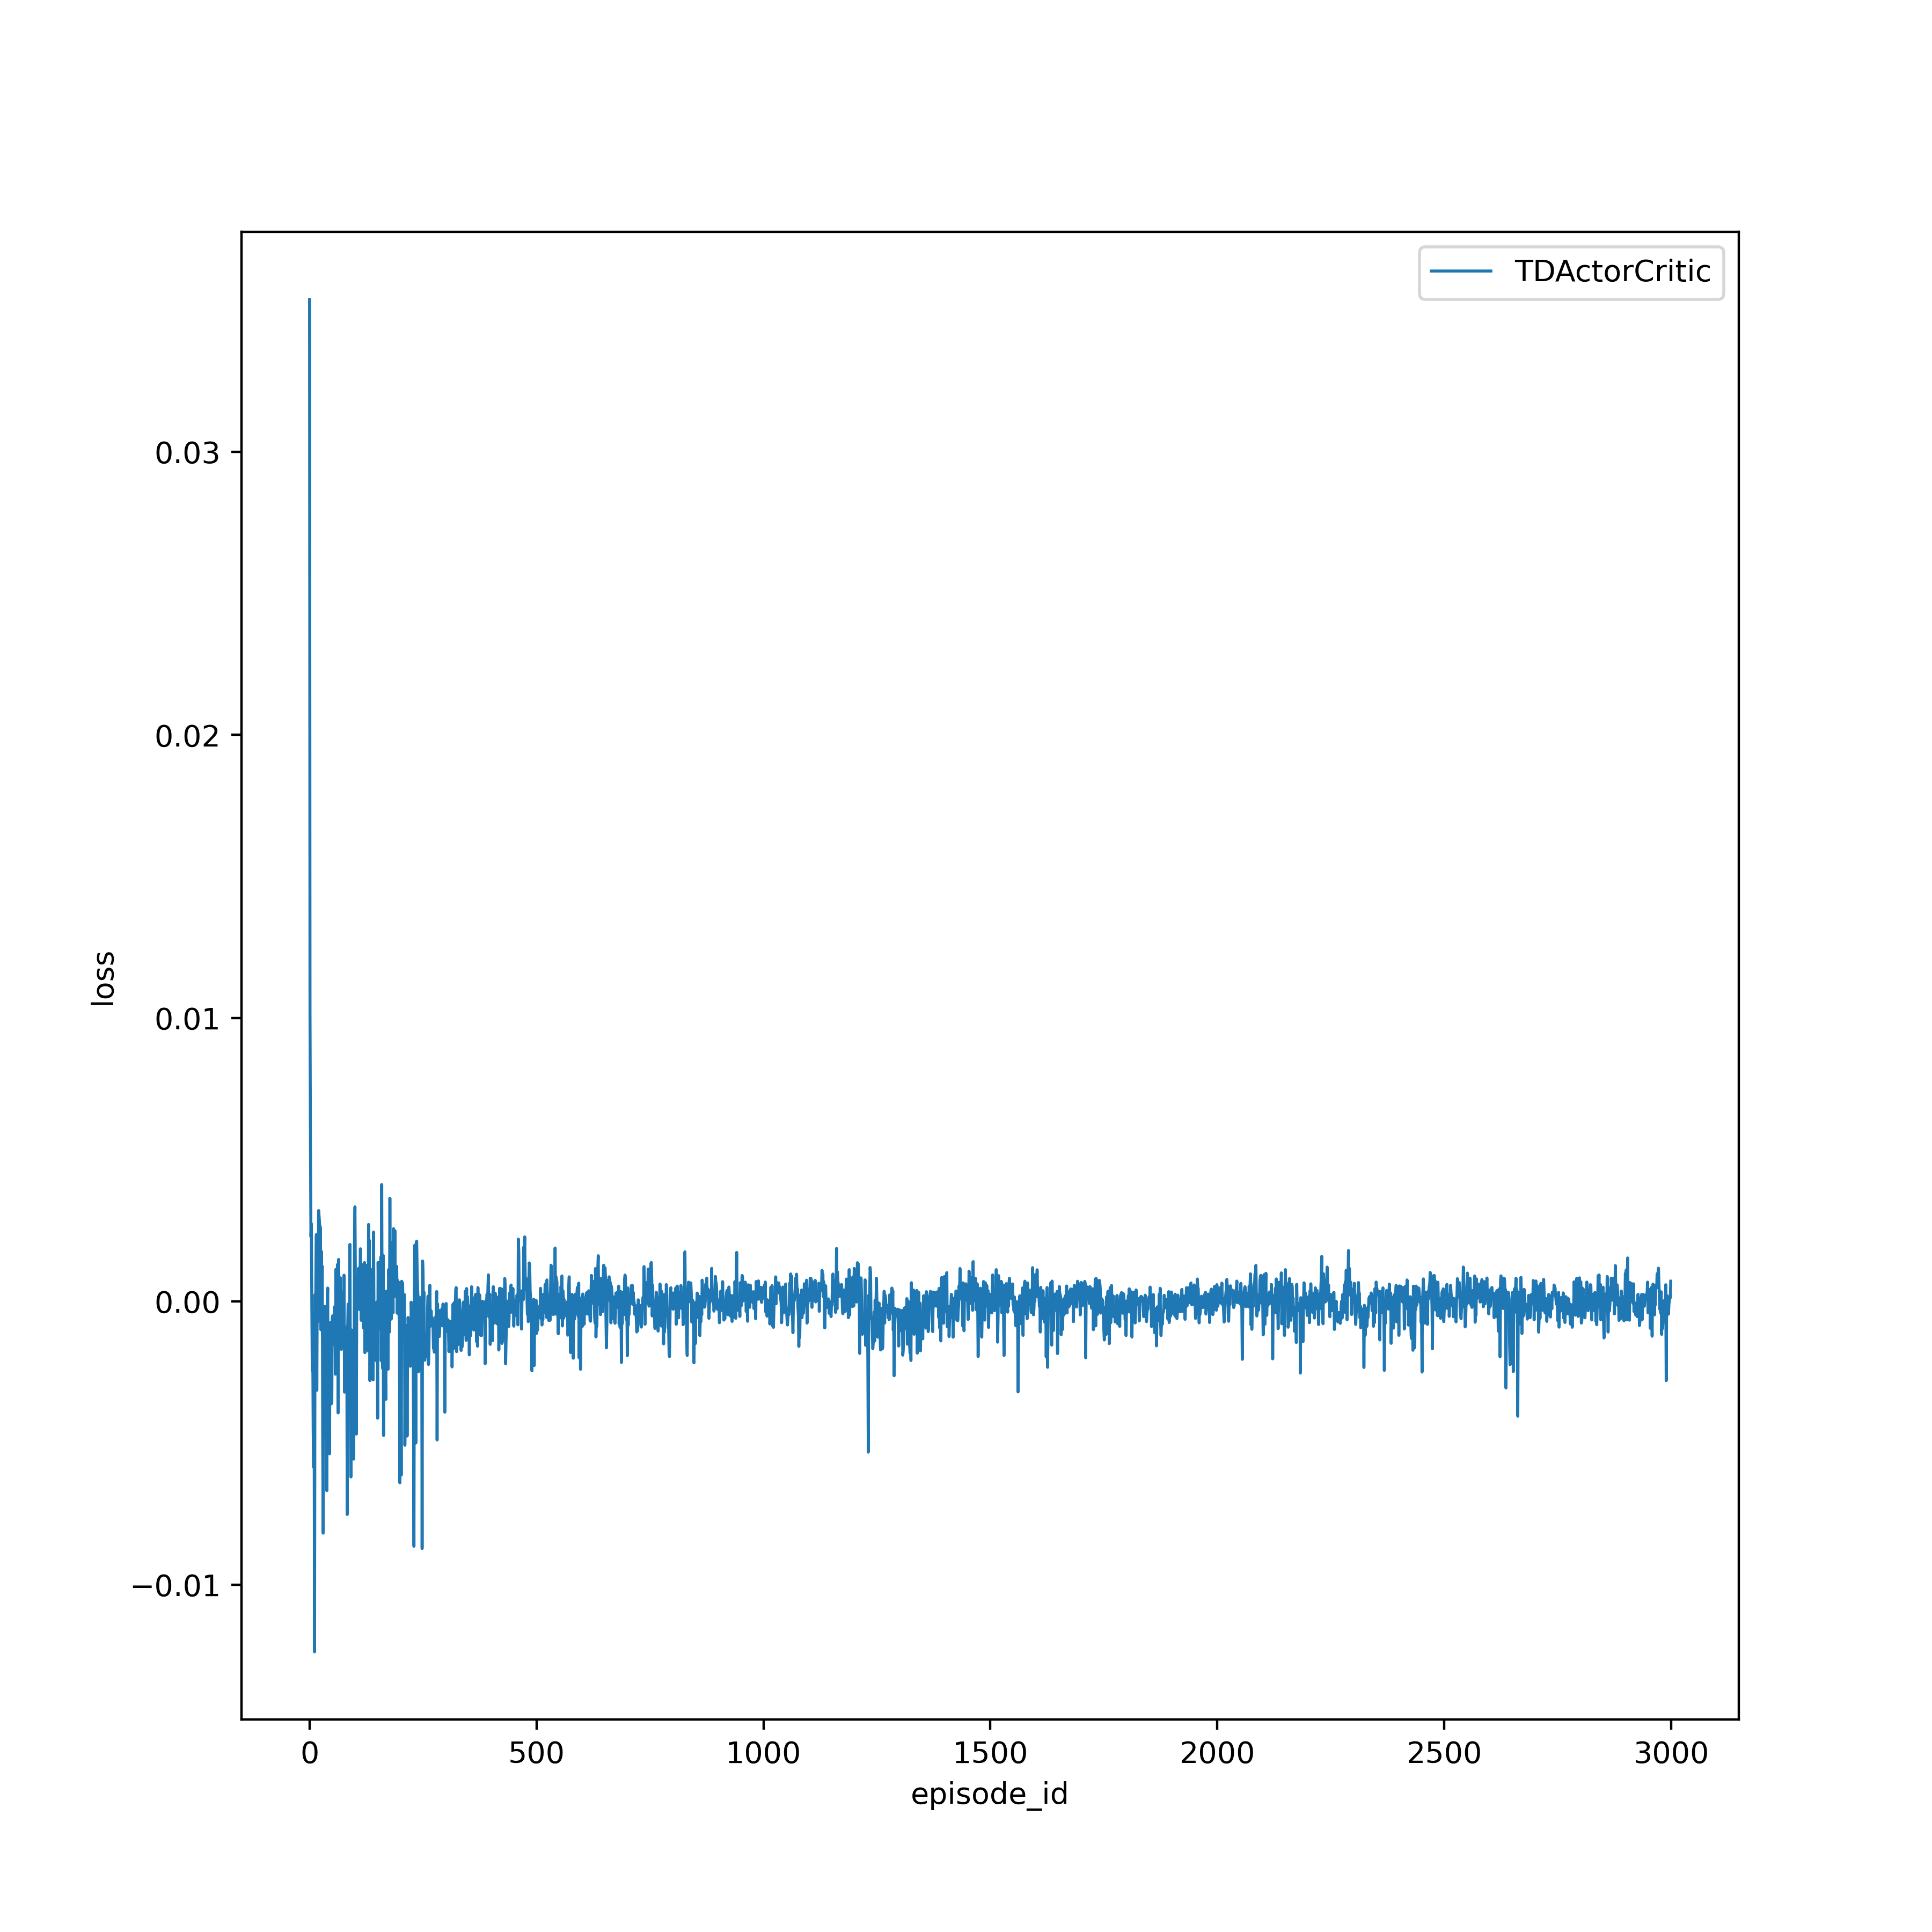
\includegraphics[width=0.40\columnwidth]{./assets/loss_TDAC (21, v0).png}}
        \subfigure[REINFORCE, seed=42]{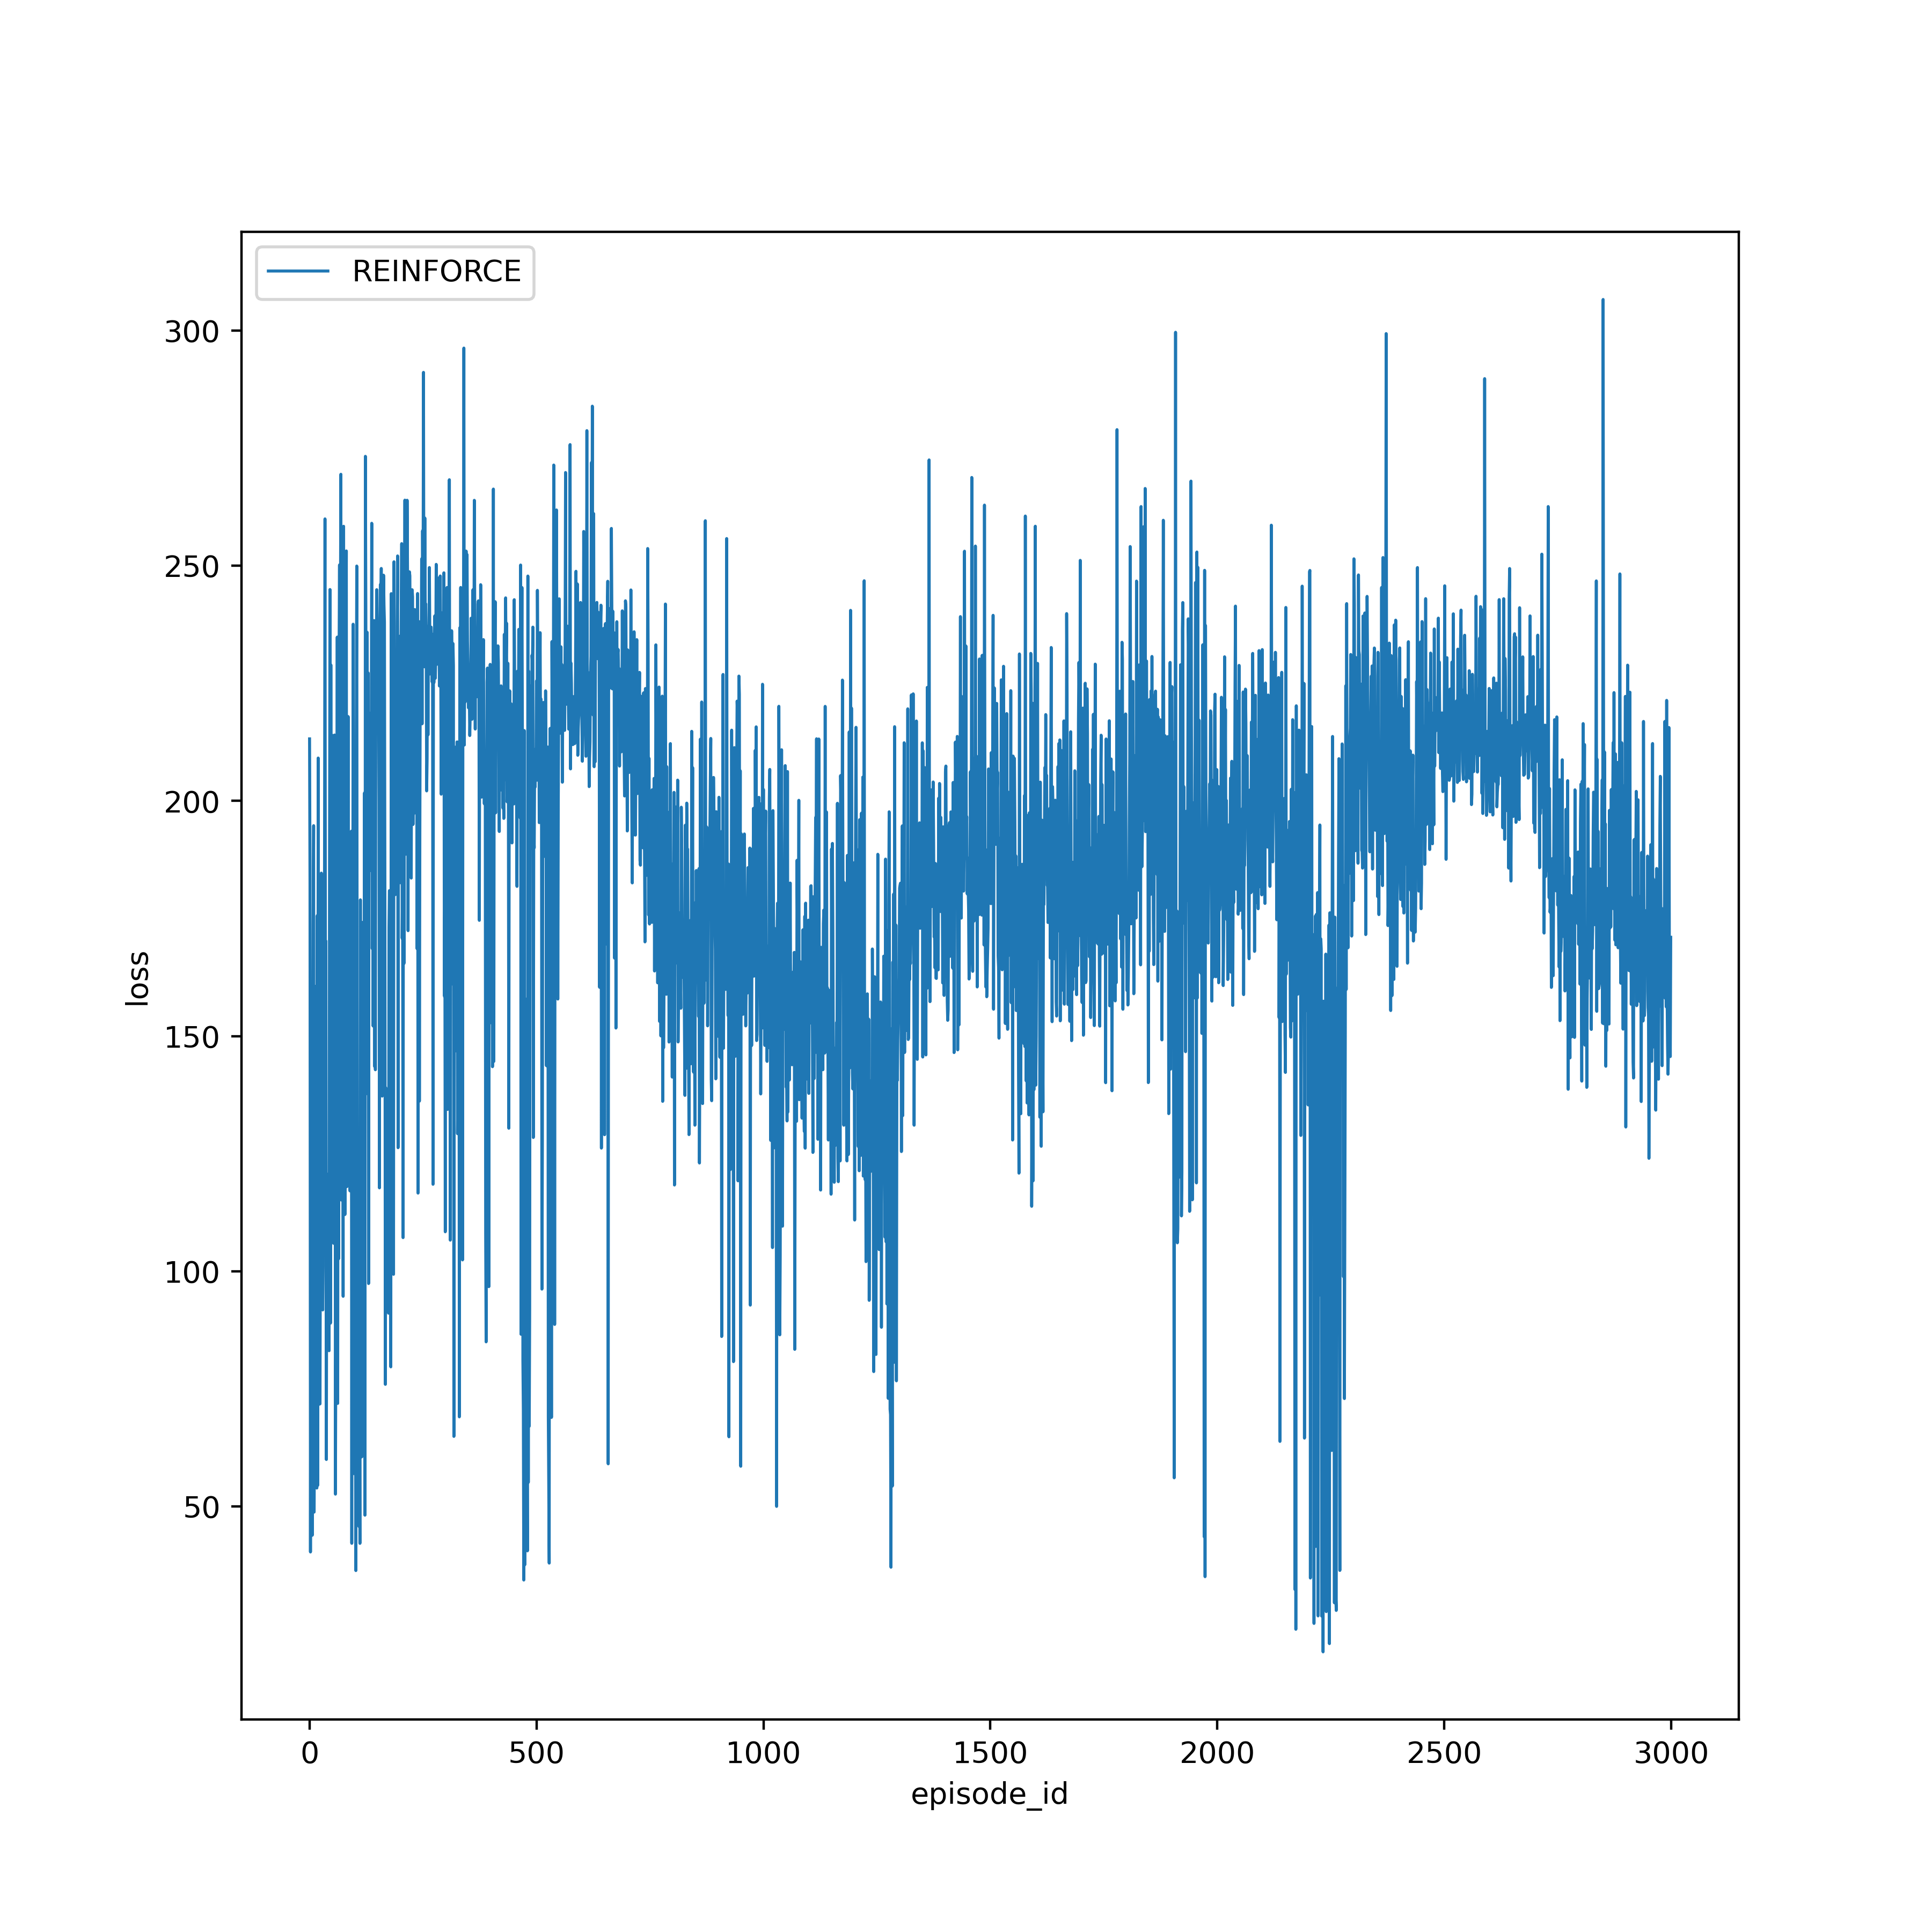
\includegraphics[width=0.40\columnwidth]{./assets/loss_REINFORCE (42, v0).png}}
        \subfigure[TDActorCritic, seed=42]{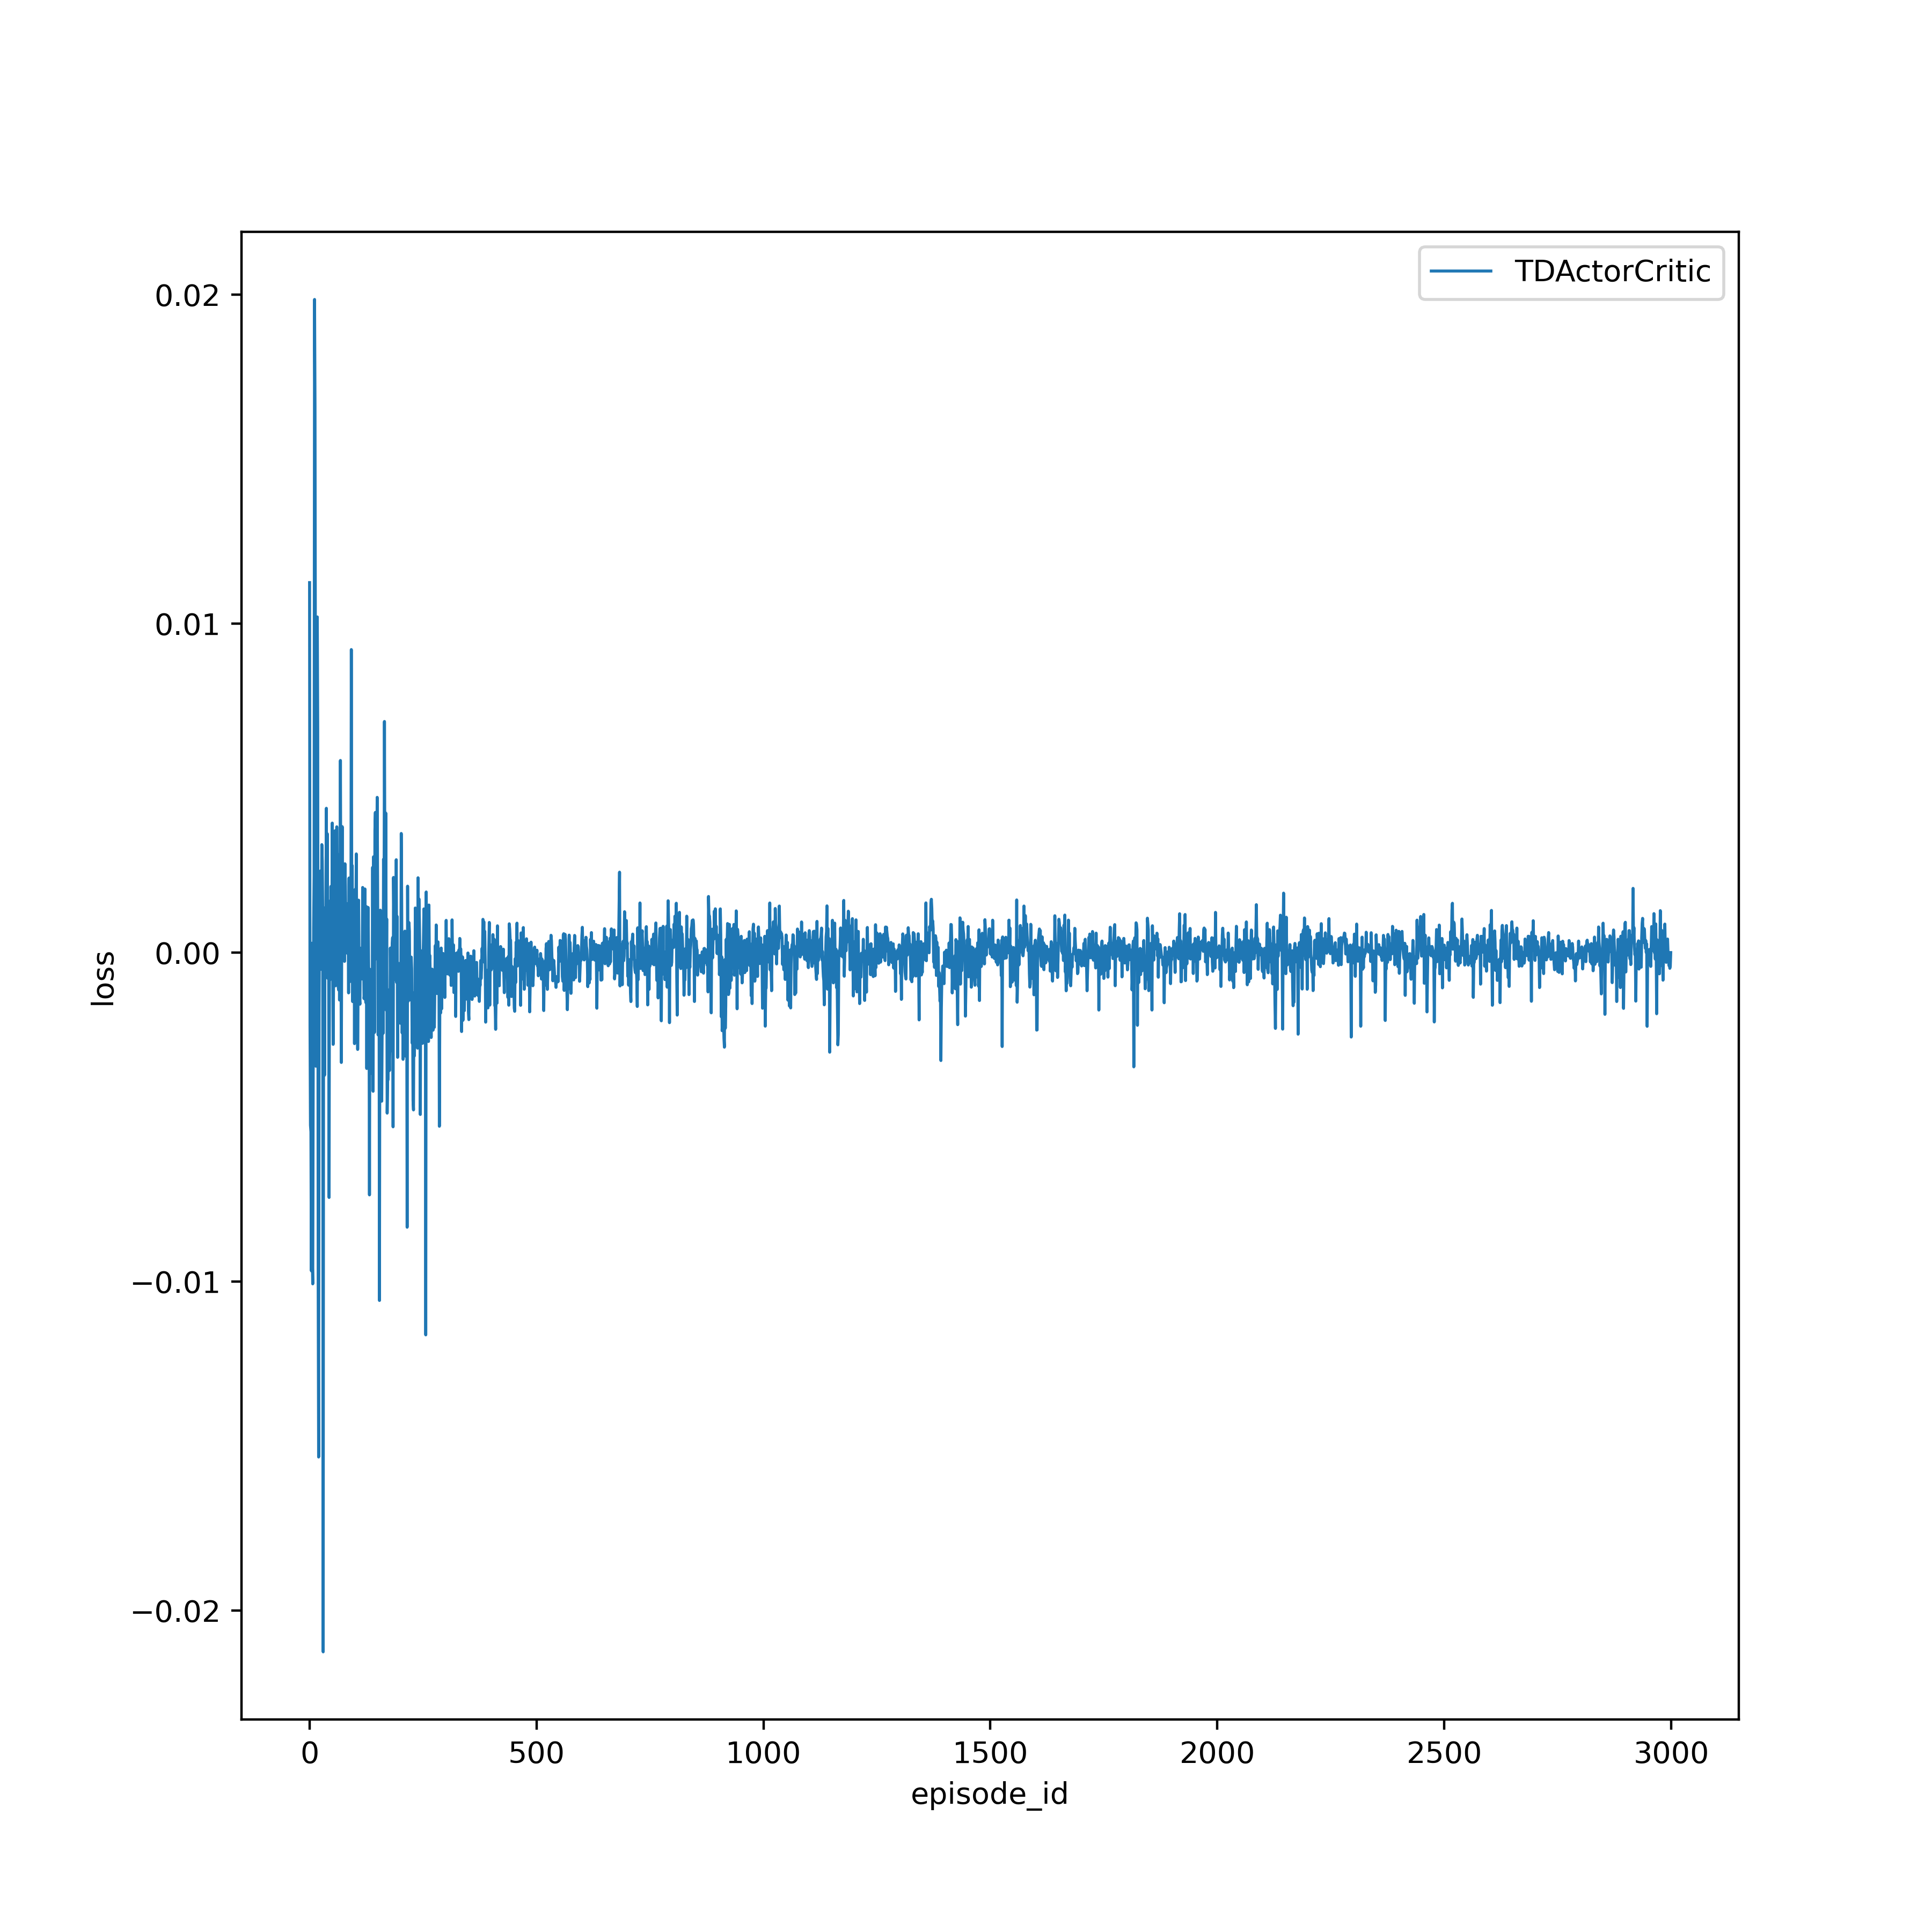
\includegraphics[width=0.40\columnwidth]{./assets/loss_TDAC (42, v0).png}}
        \caption{两模型在cartpole-v0环境训练中的损失值变化情况}
        \end{figure}

        \begin{figure}[htbp]
        \centering
        \subfigure[REINFORCE, seed=0]{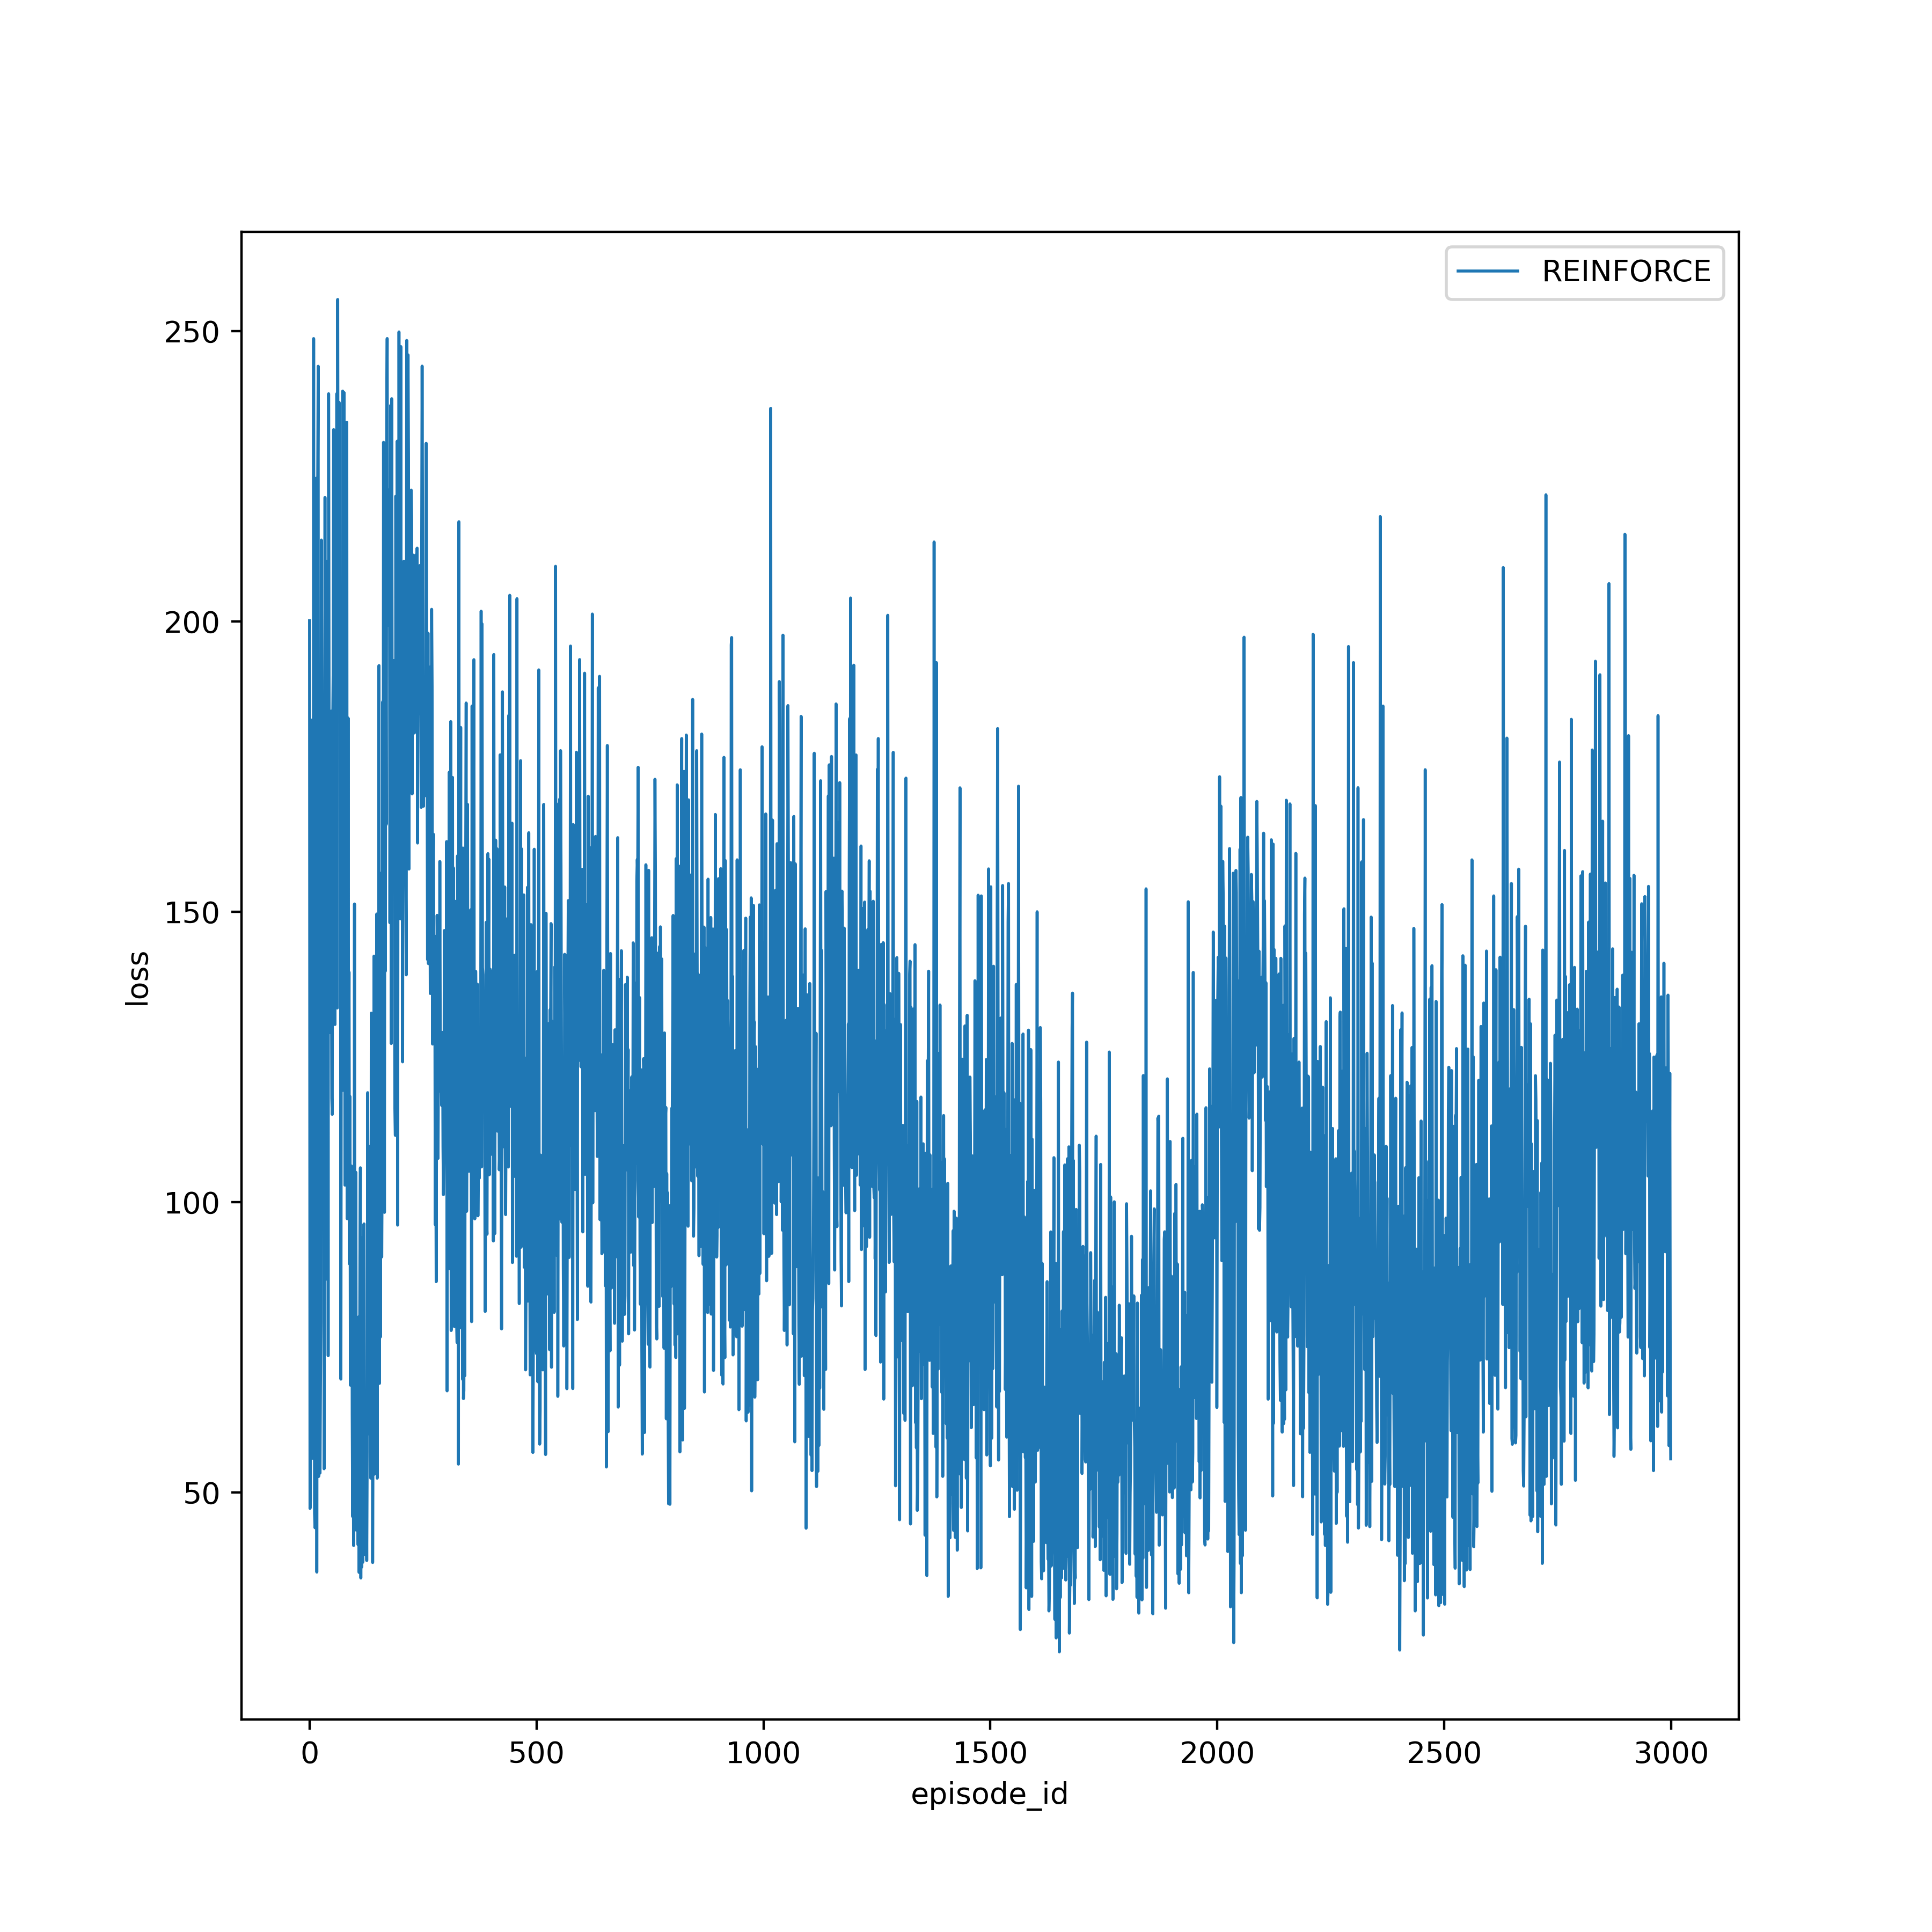
\includegraphics[width=0.40\columnwidth]{./assets/loss_REINFORCE (0, v1).png}}
        \subfigure[TDActorCritic, seed=0]{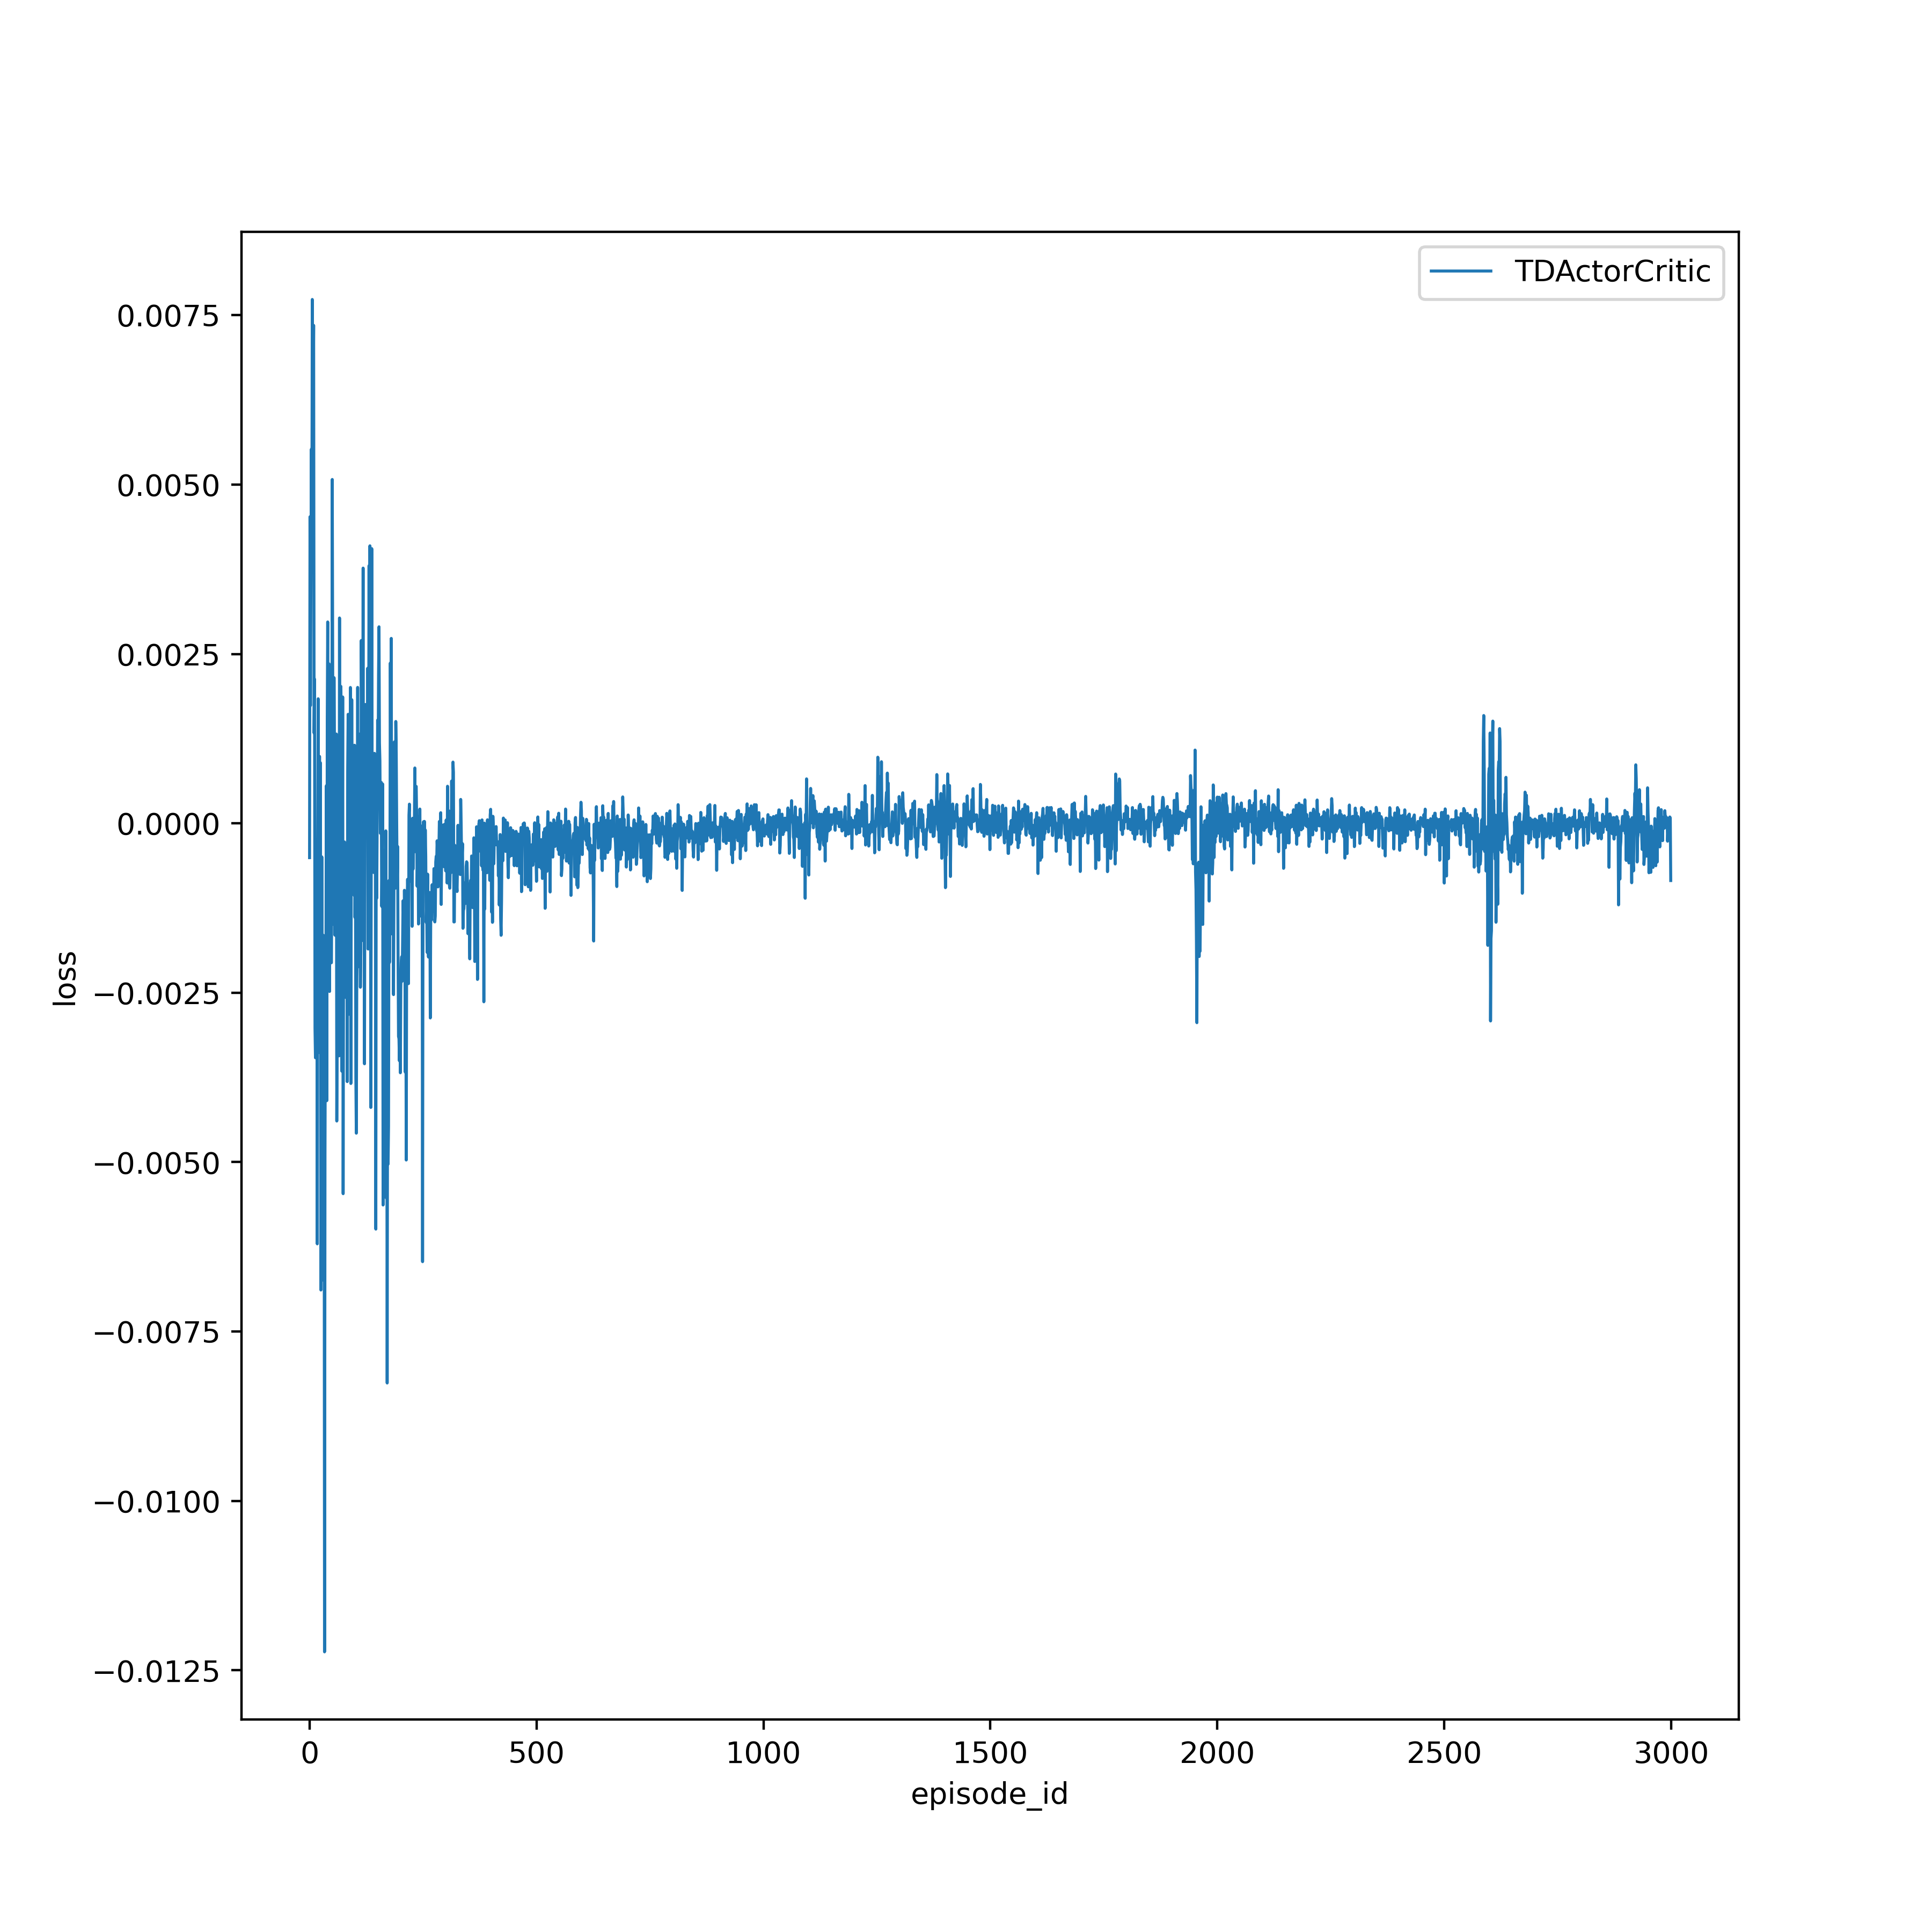
\includegraphics[width=0.40\columnwidth]{./assets/loss_TDAC (0, v1).png}}
        \subfigure[REINFORCE, seed=21]{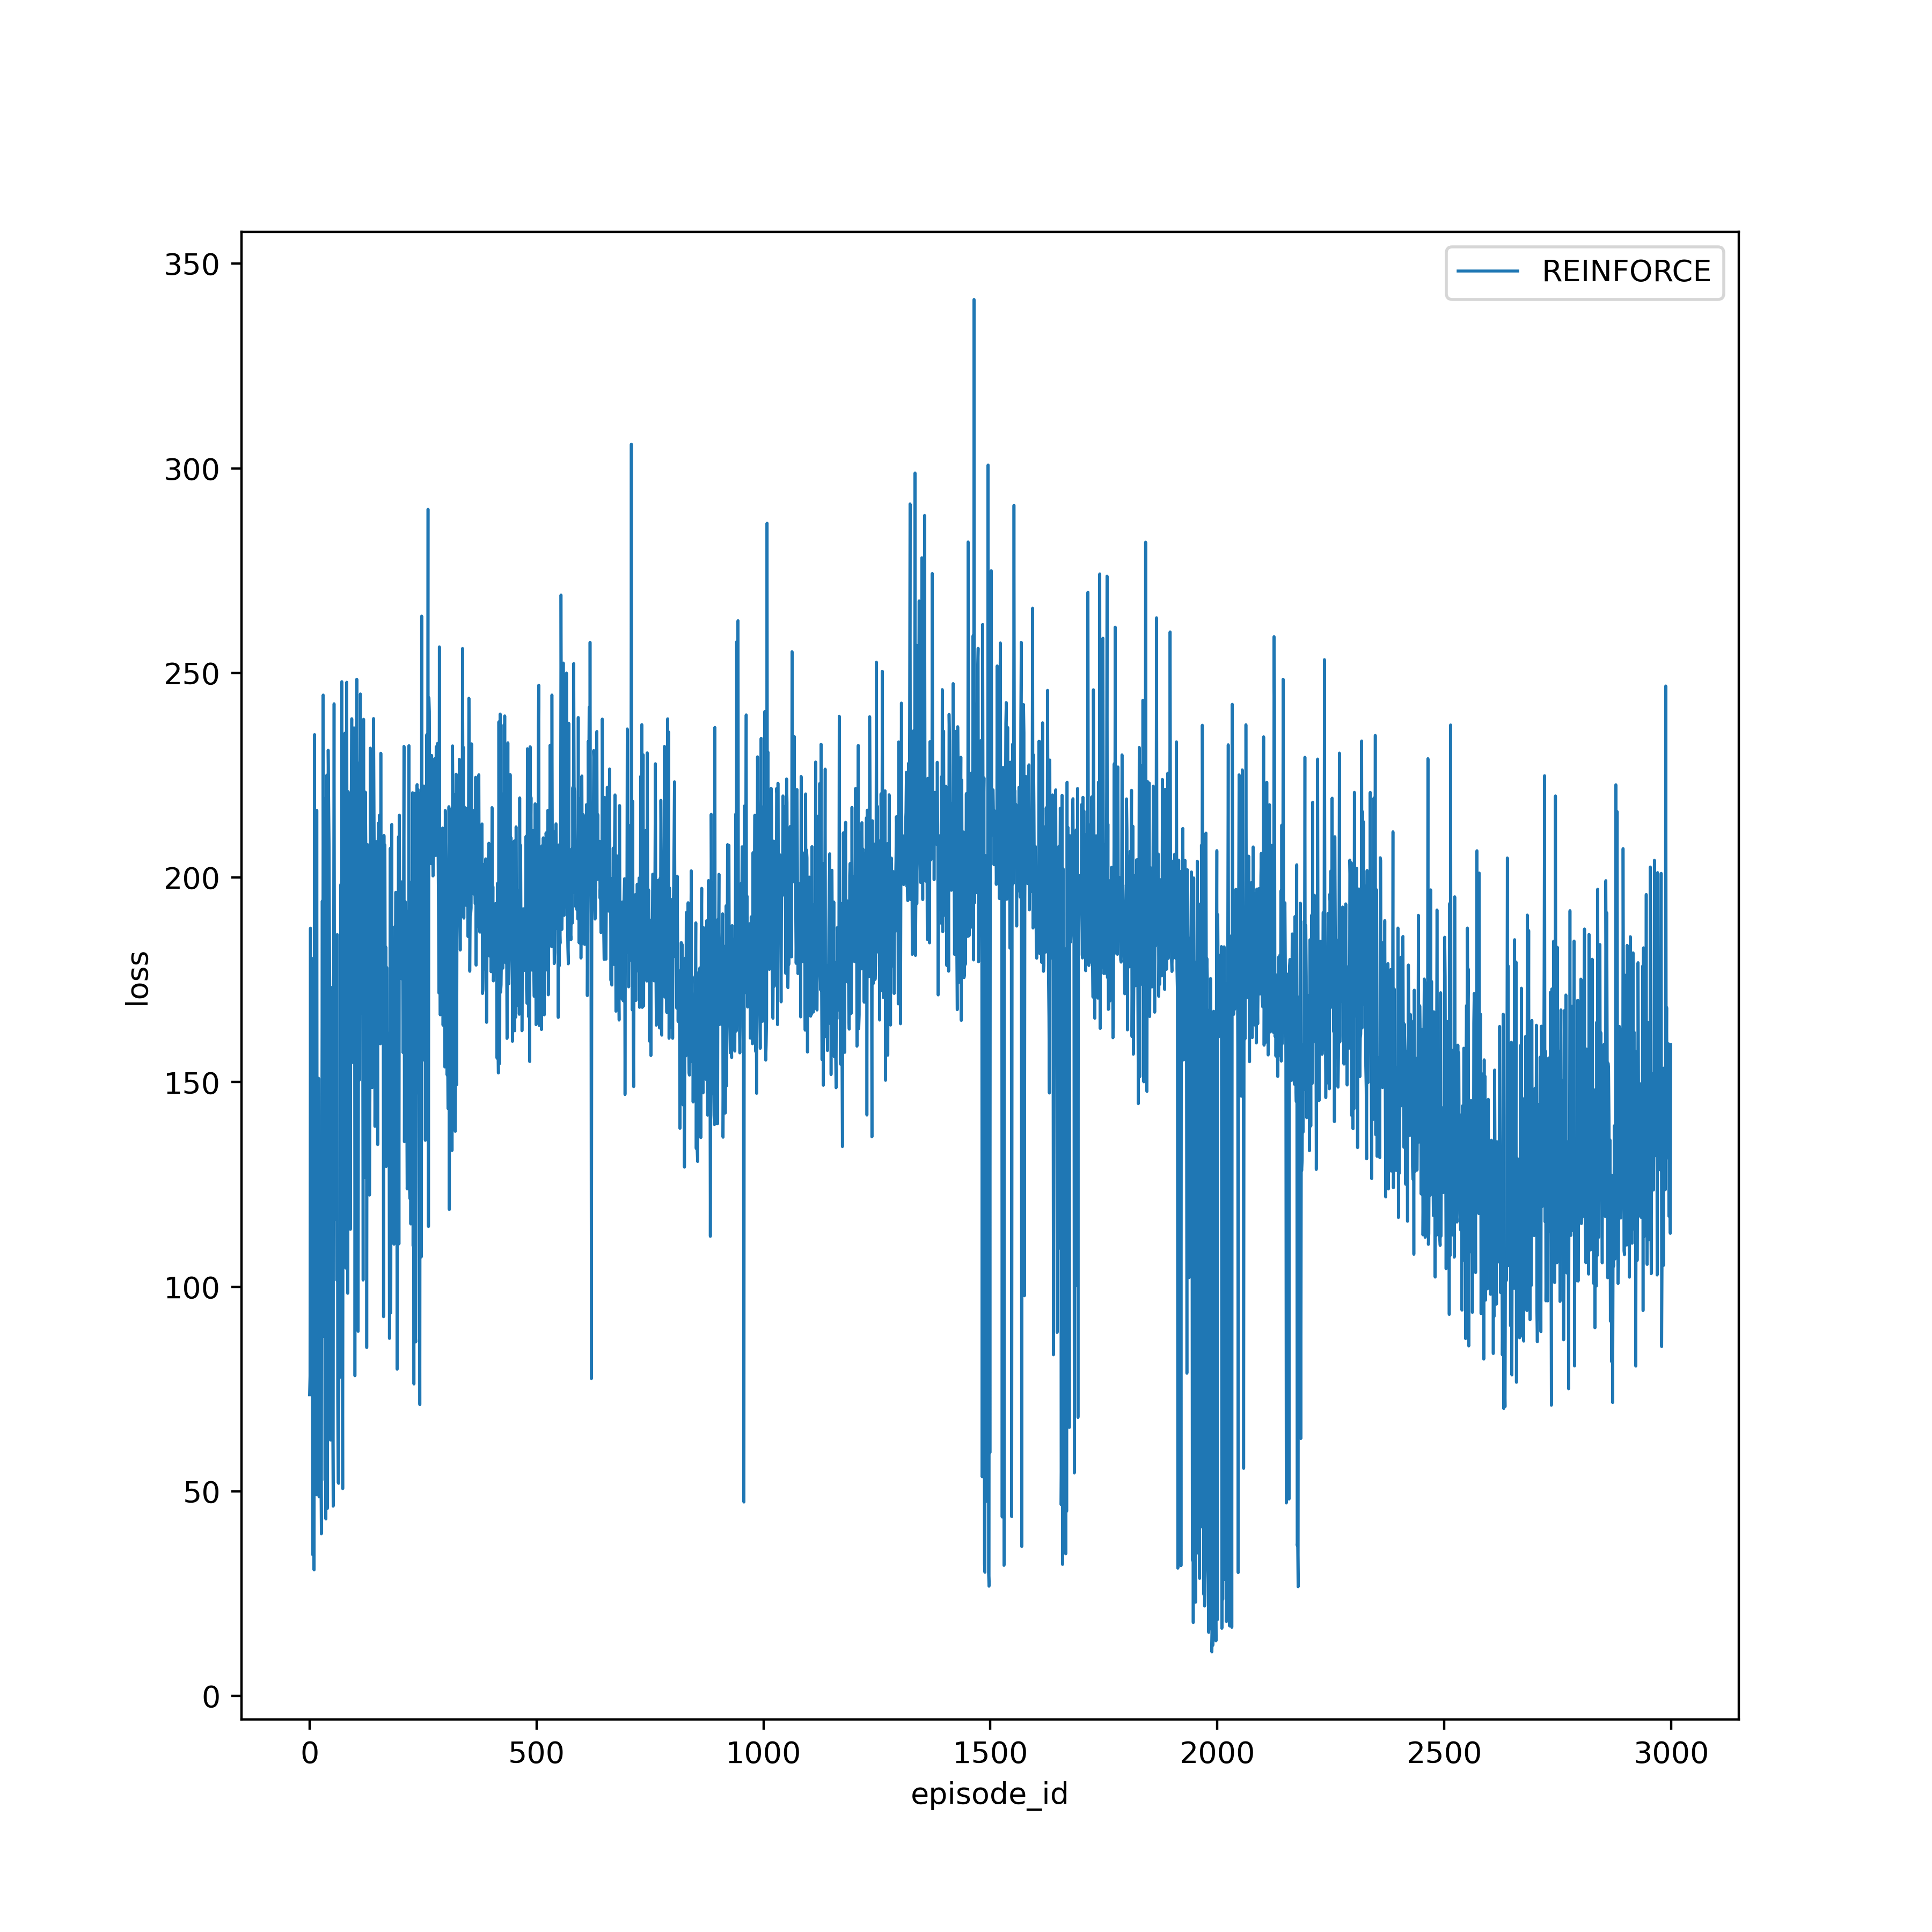
\includegraphics[width=0.40\columnwidth]{./assets/loss_REINFORCE (21, v1).png}}
        \subfigure[TDActorCritic, seed=21]{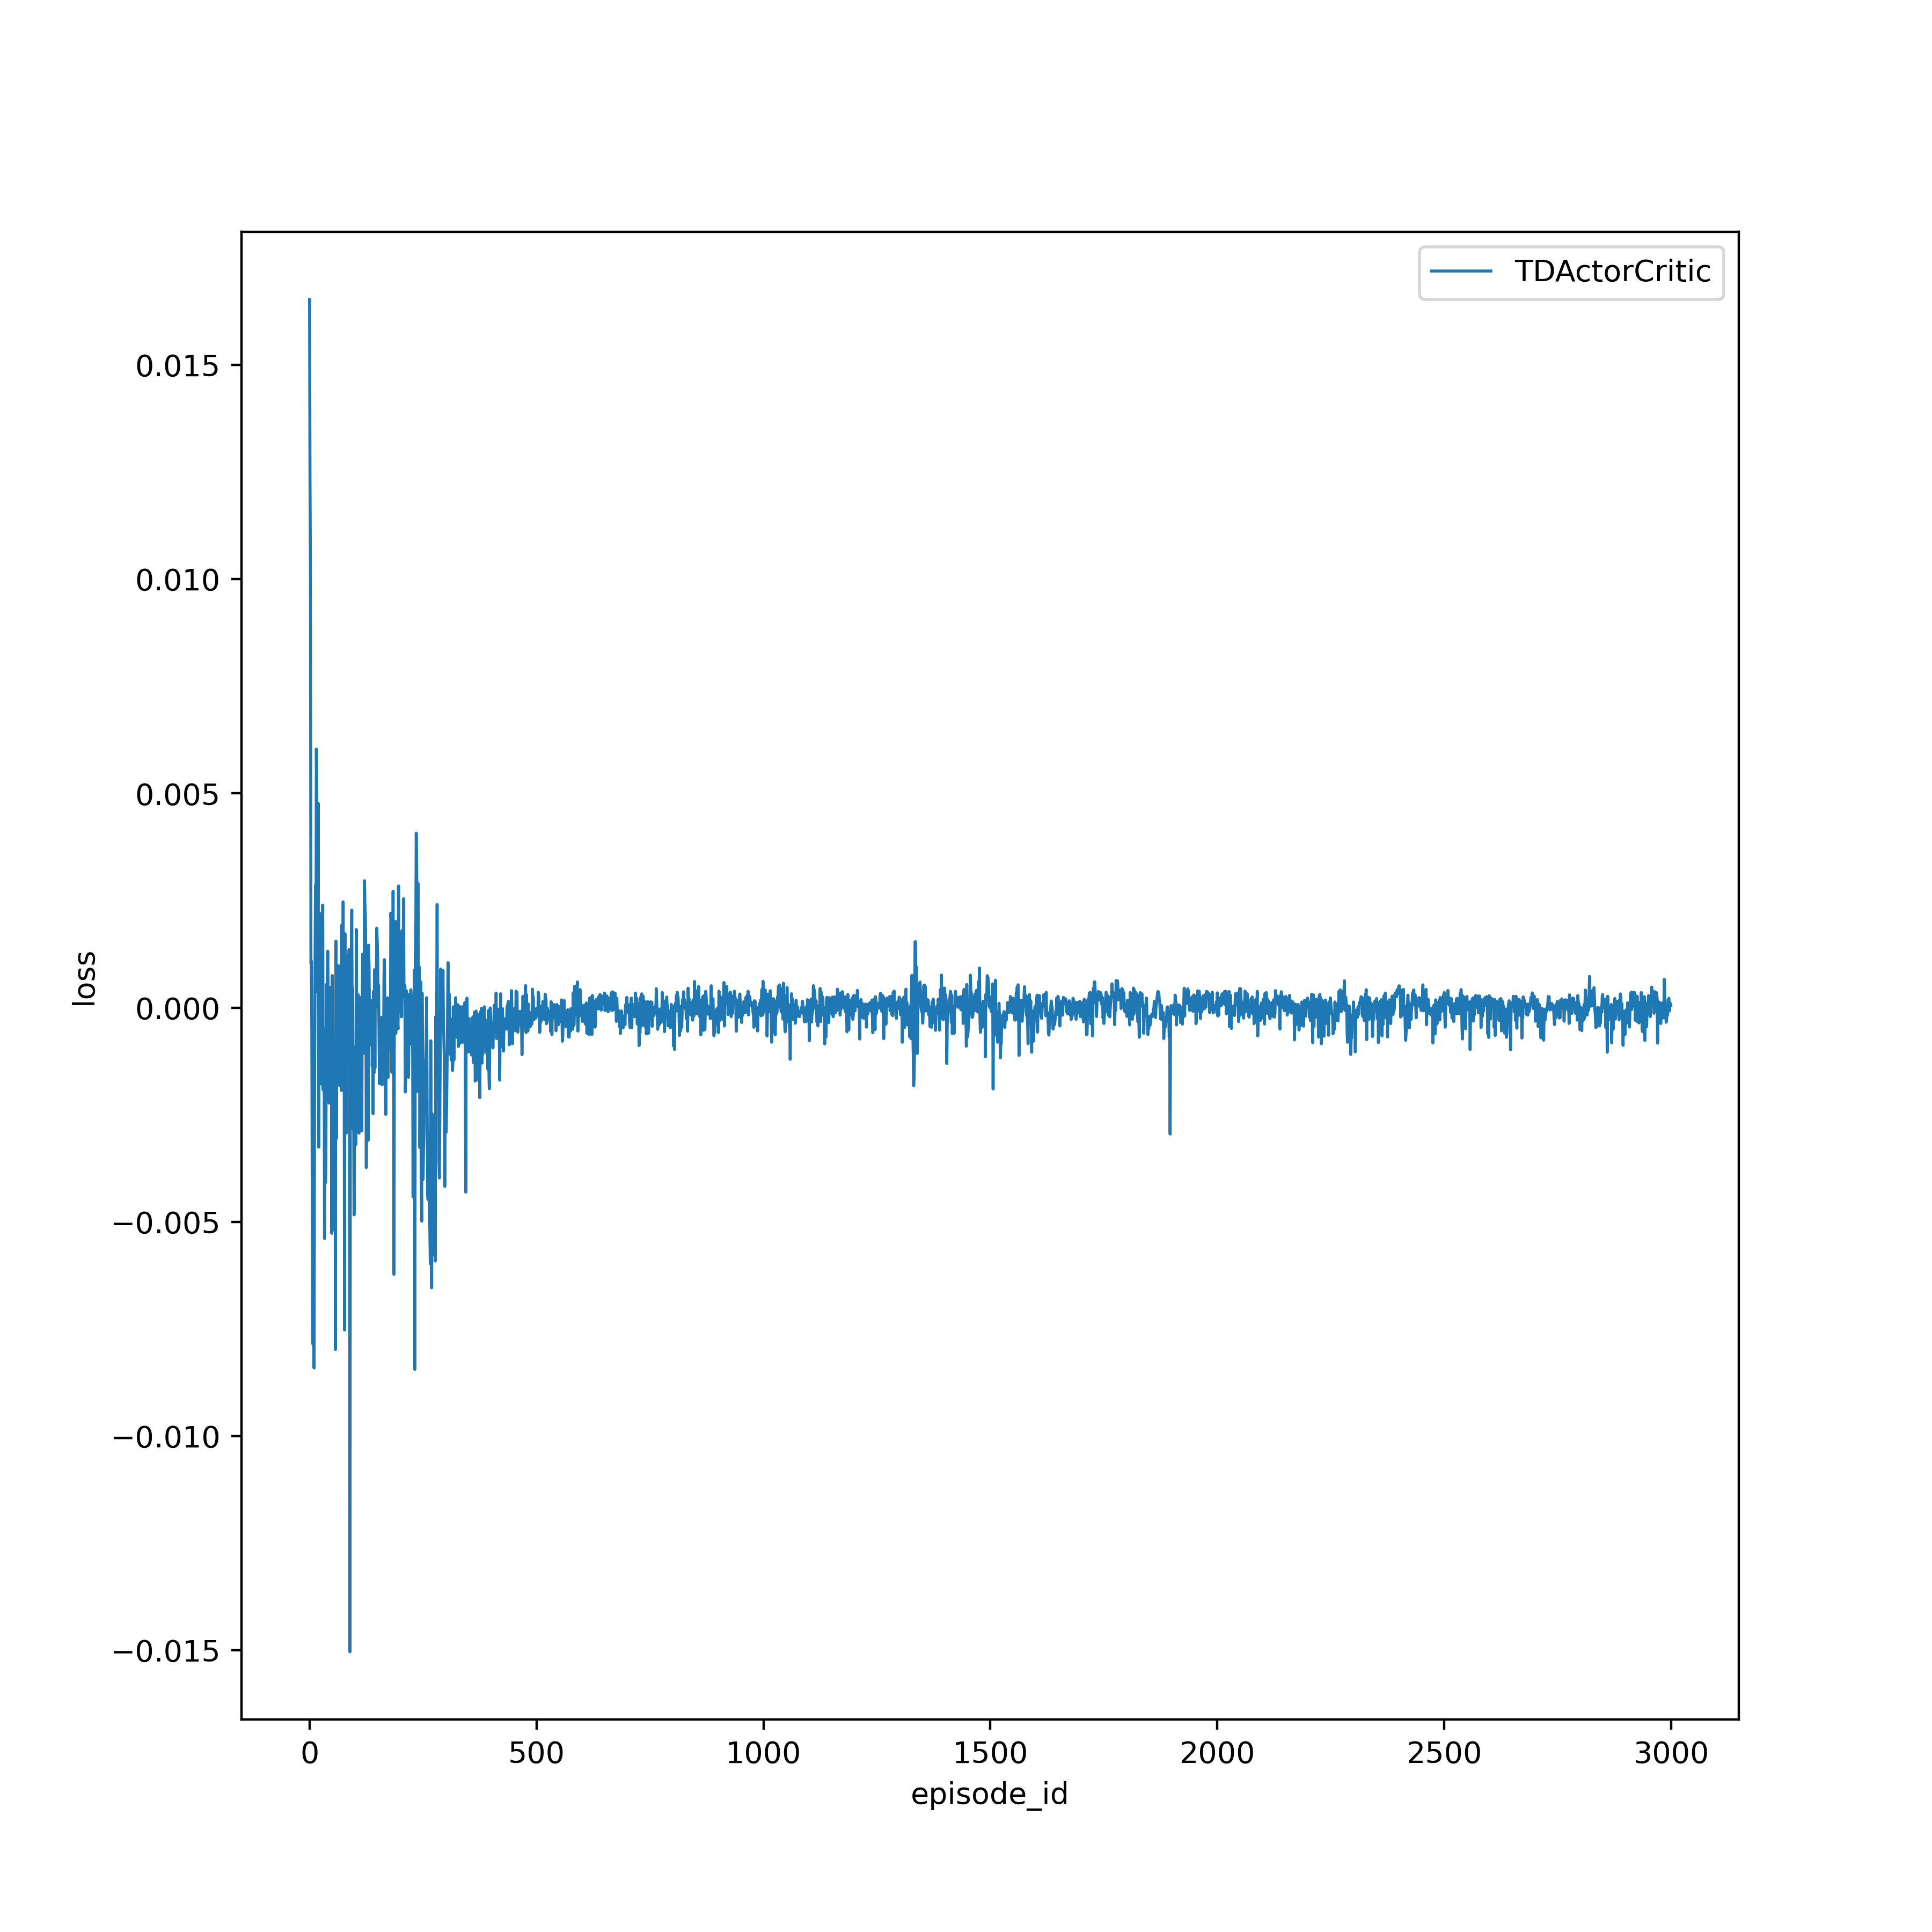
\includegraphics[width=0.40\columnwidth]{./assets/loss_TDAC (21, v1).png}}
        \subfigure[REINFORCE, seed=42]{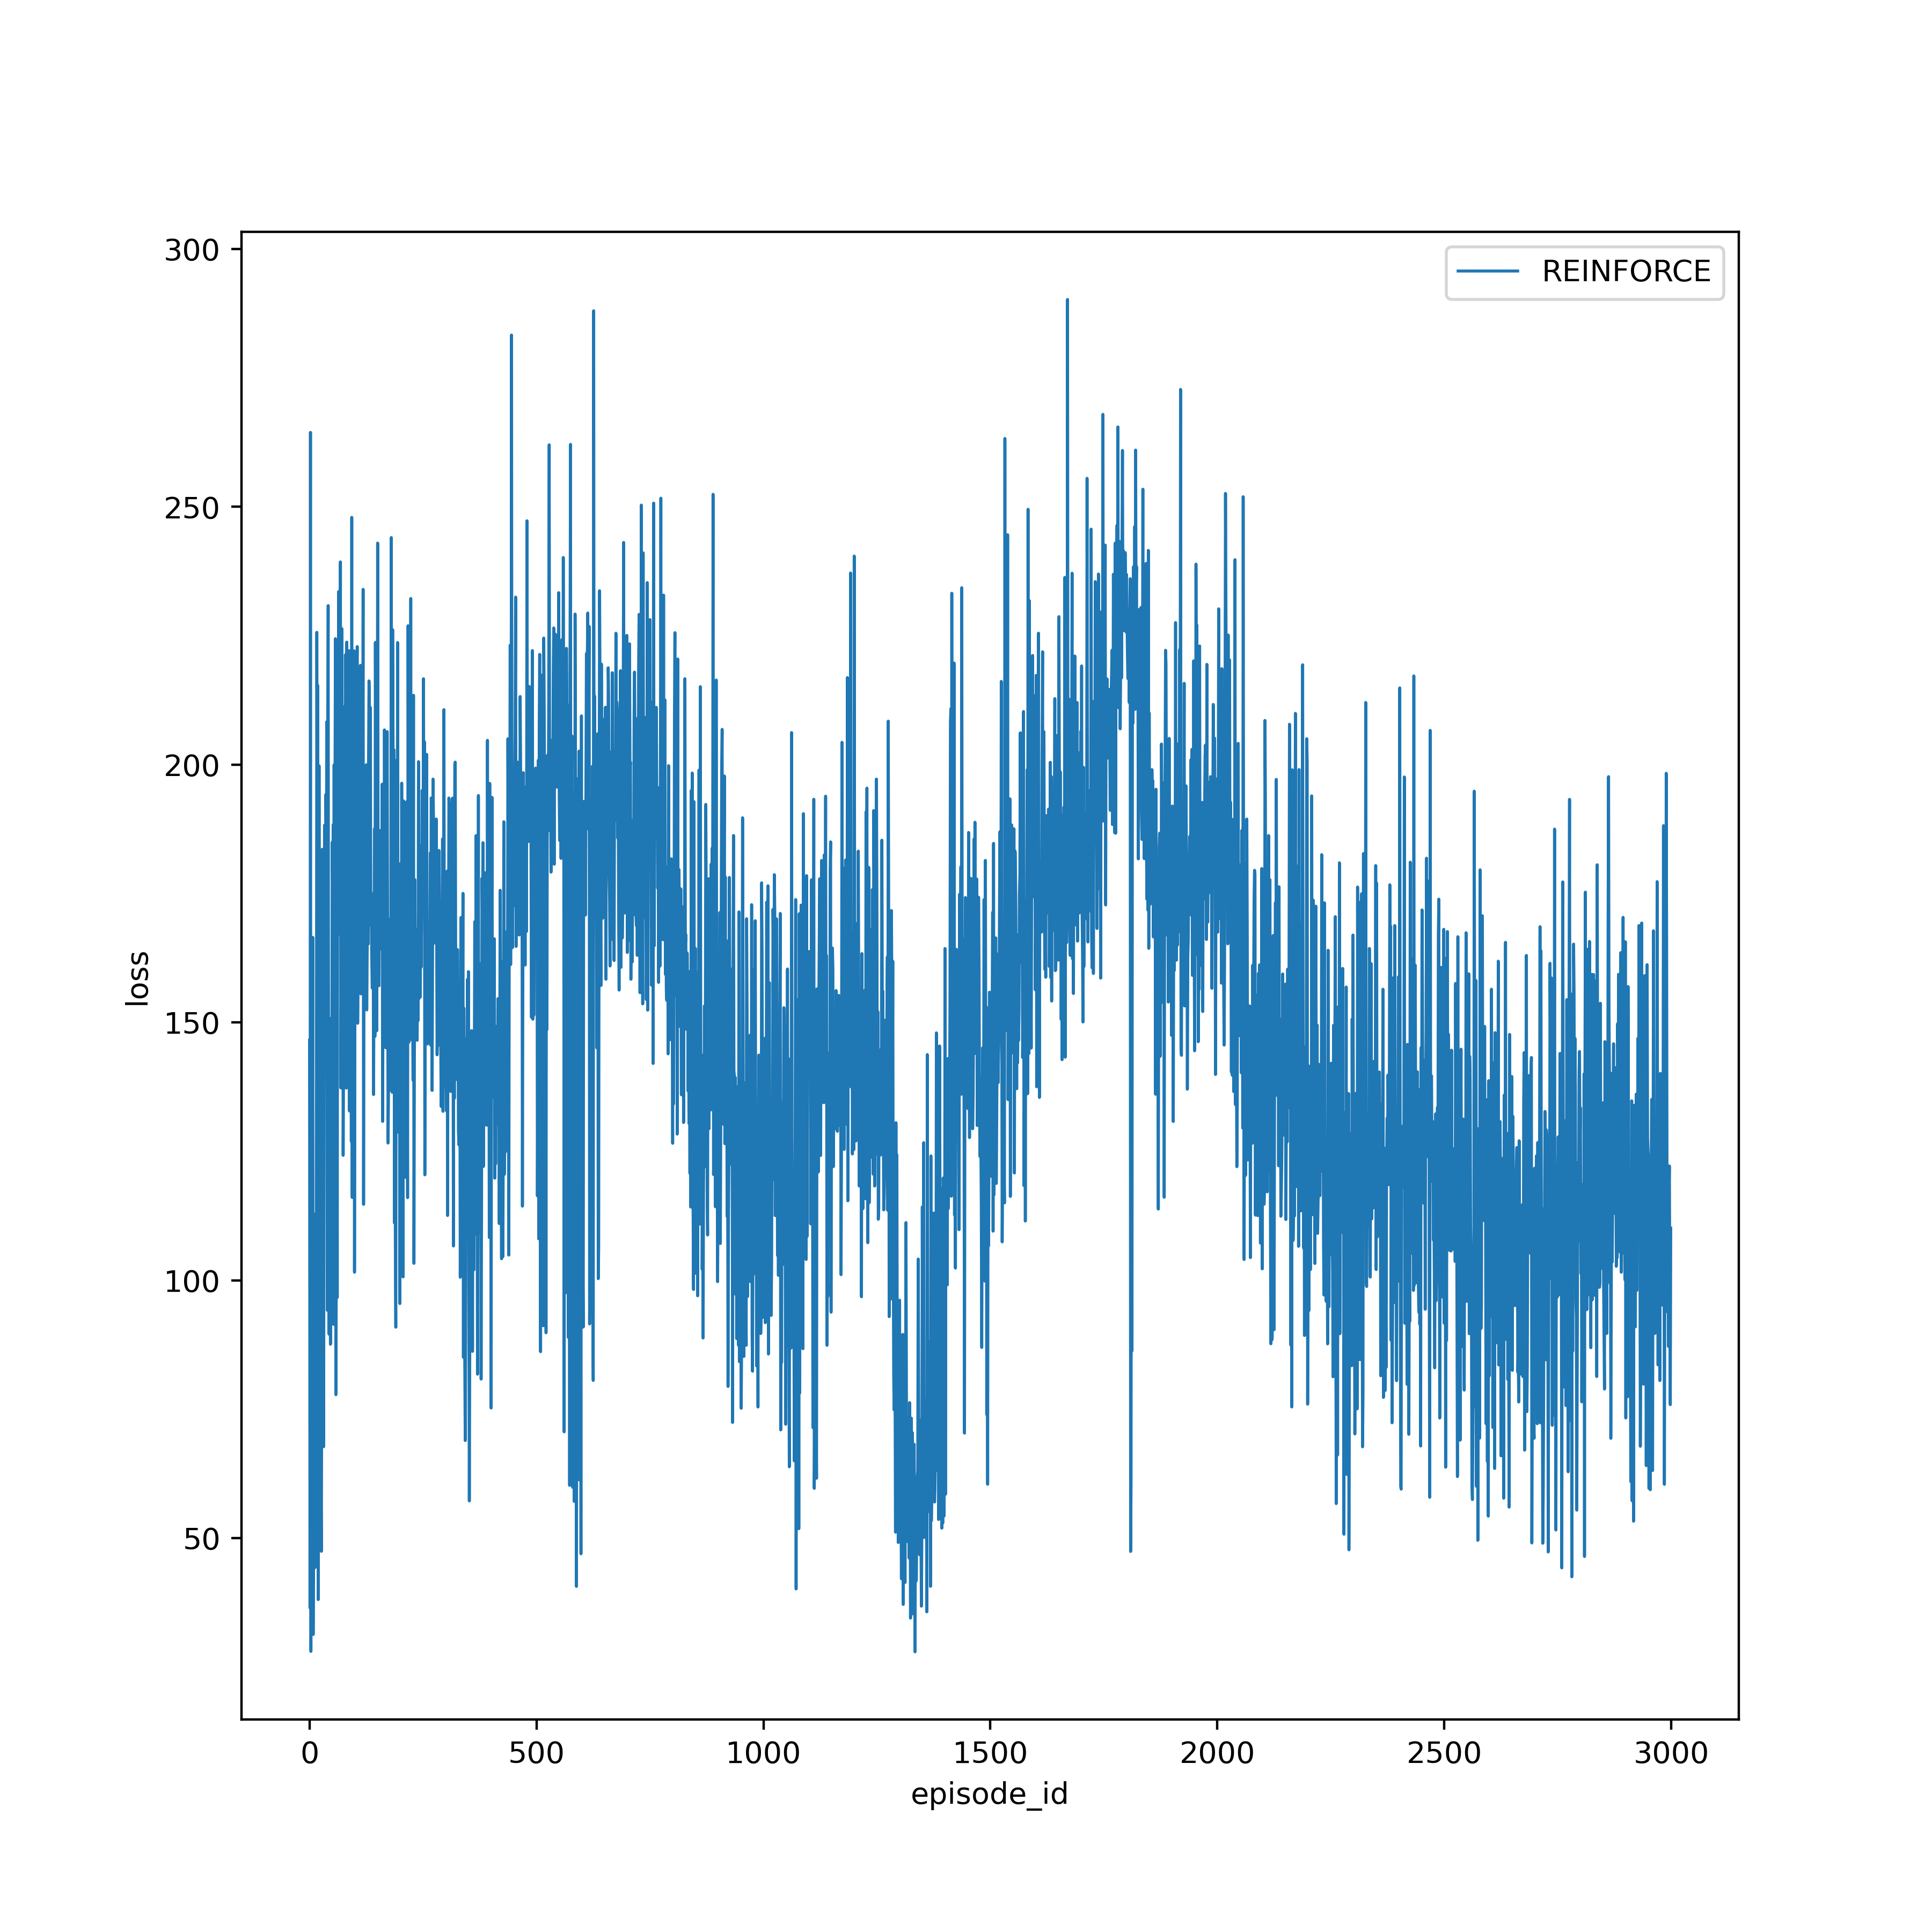
\includegraphics[width=0.40\columnwidth]{./assets/loss_REINFORCE (42, v1).png}}
        \subfigure[TDActorCritic, seed=42]{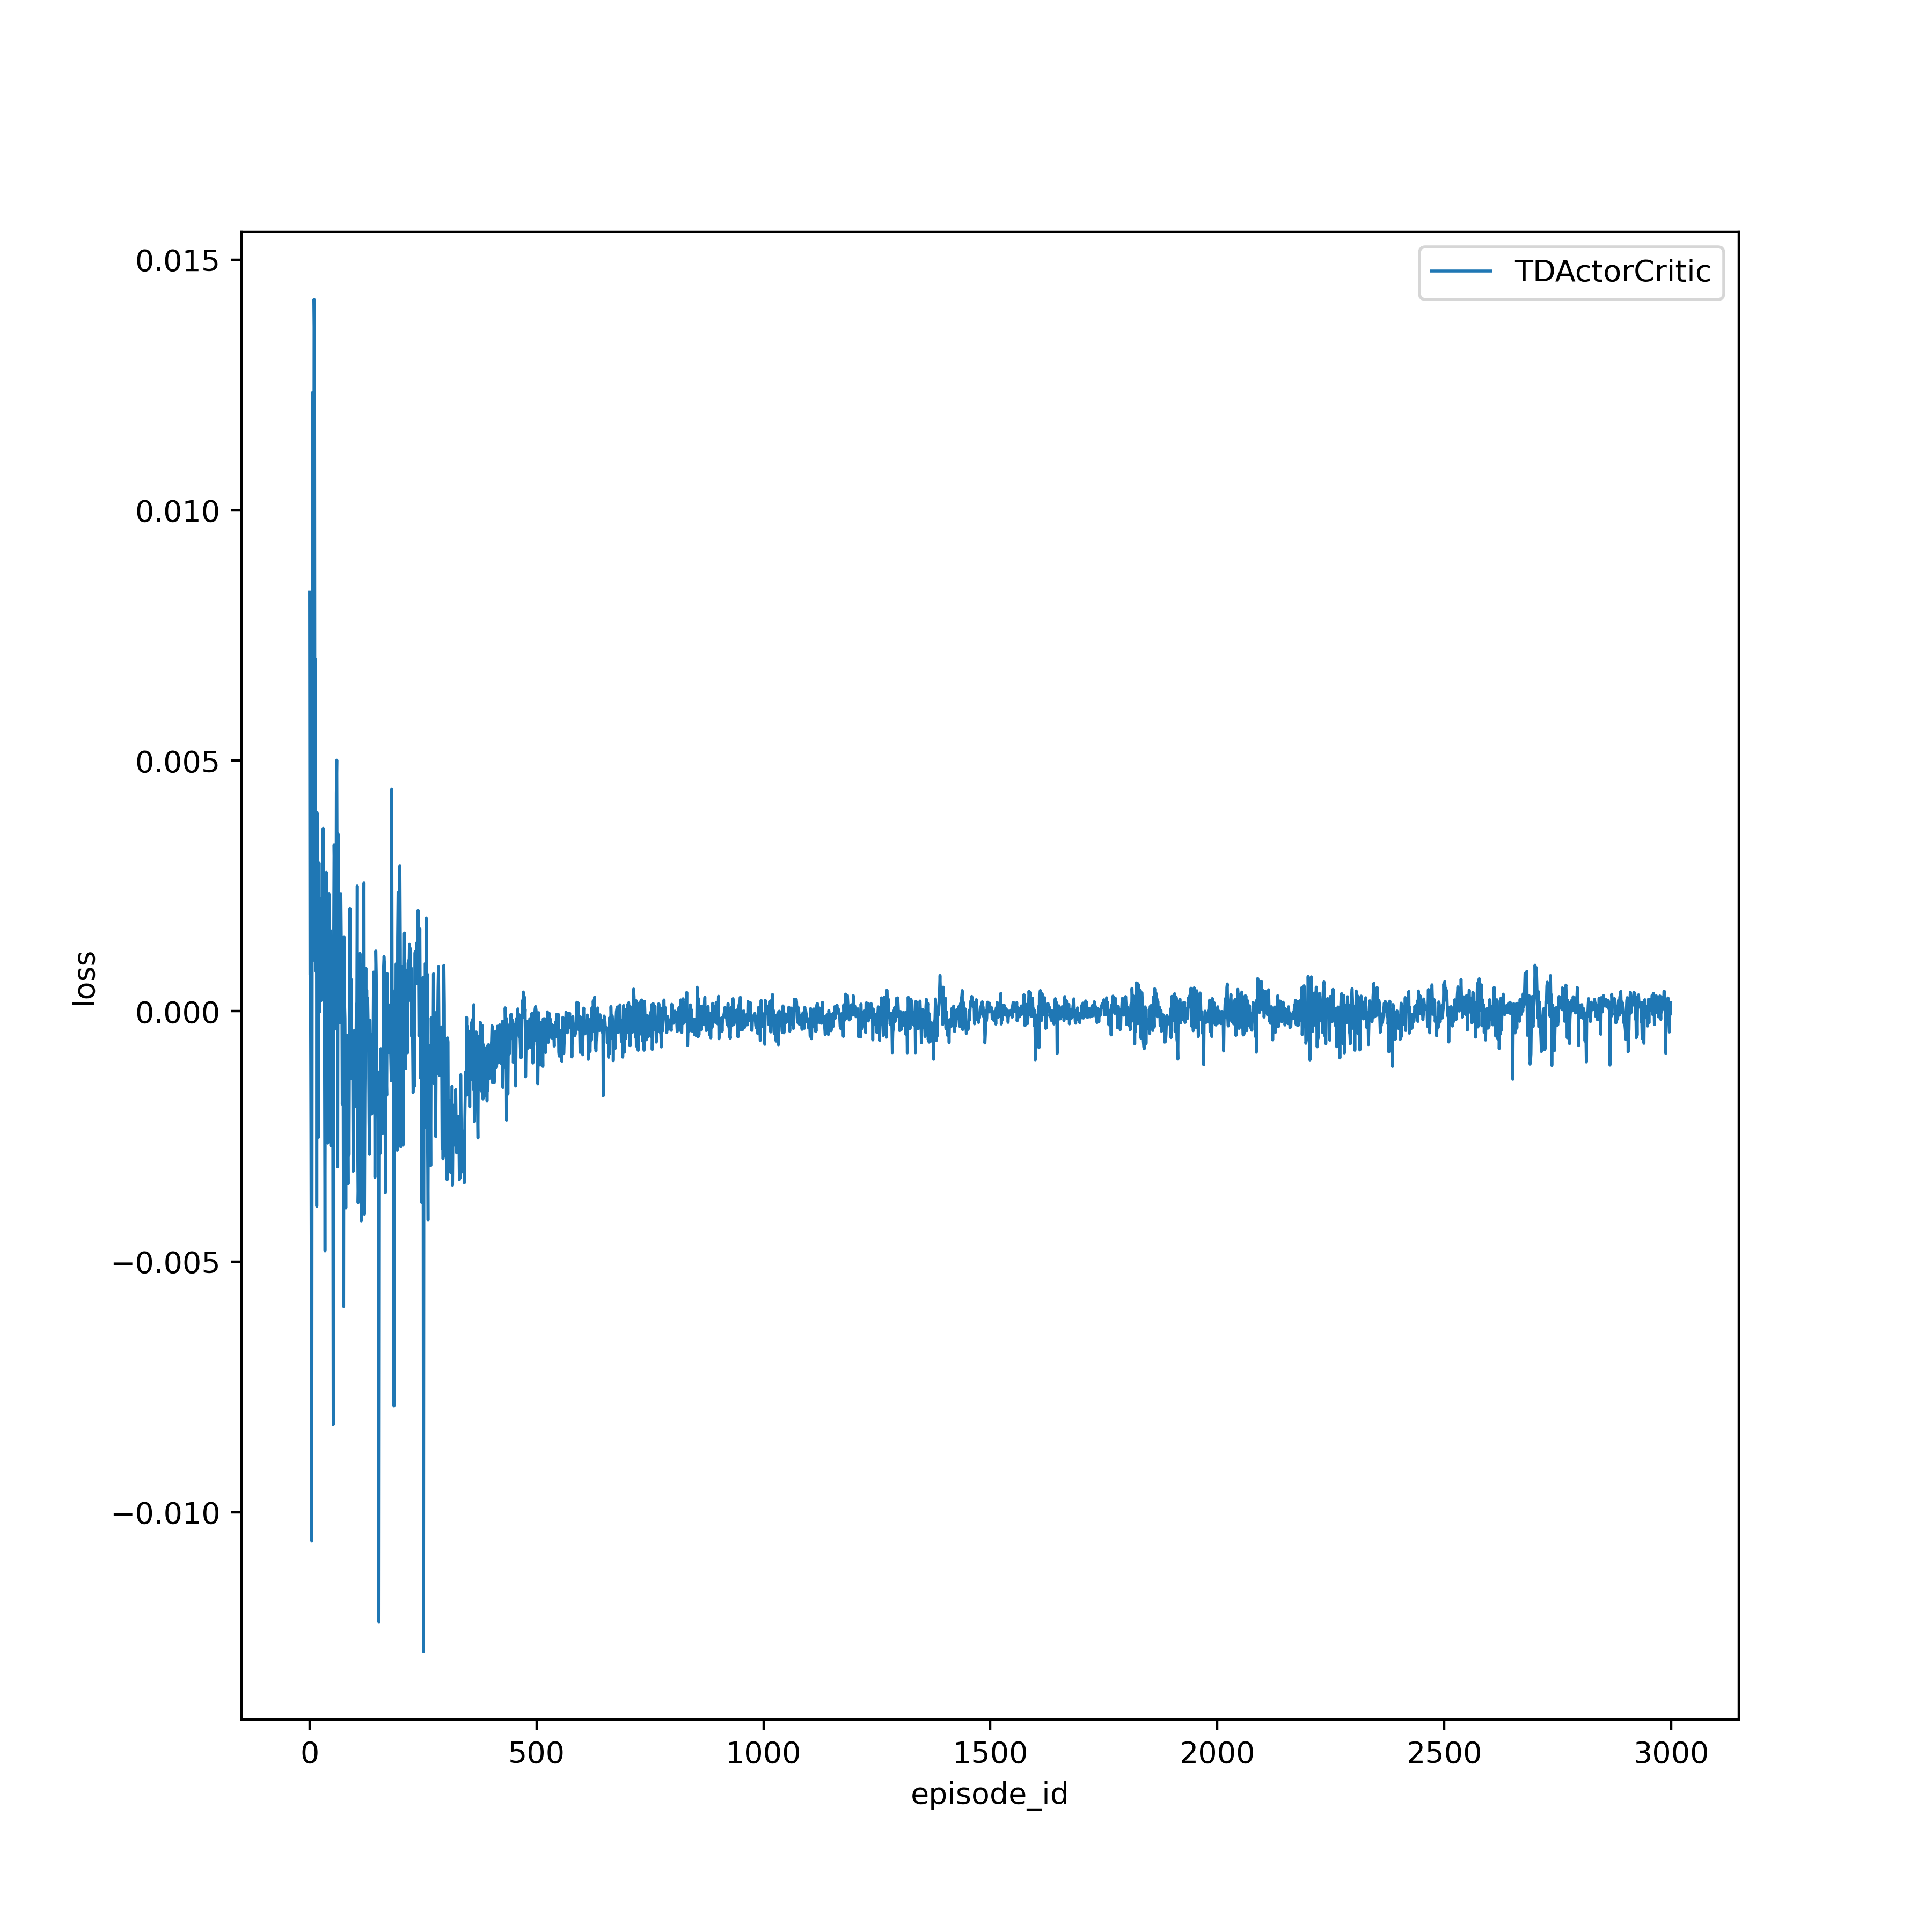
\includegraphics[width=0.40\columnwidth]{./assets/loss_TDAC (42, v1).png}}
        \caption{两模型在cartpole-v1环境训练中的损失值变化情况}
        \end{figure}

        \begin{figure}[htbp]
        \centering
        \subfigure[cartpole-v0, seed=0]{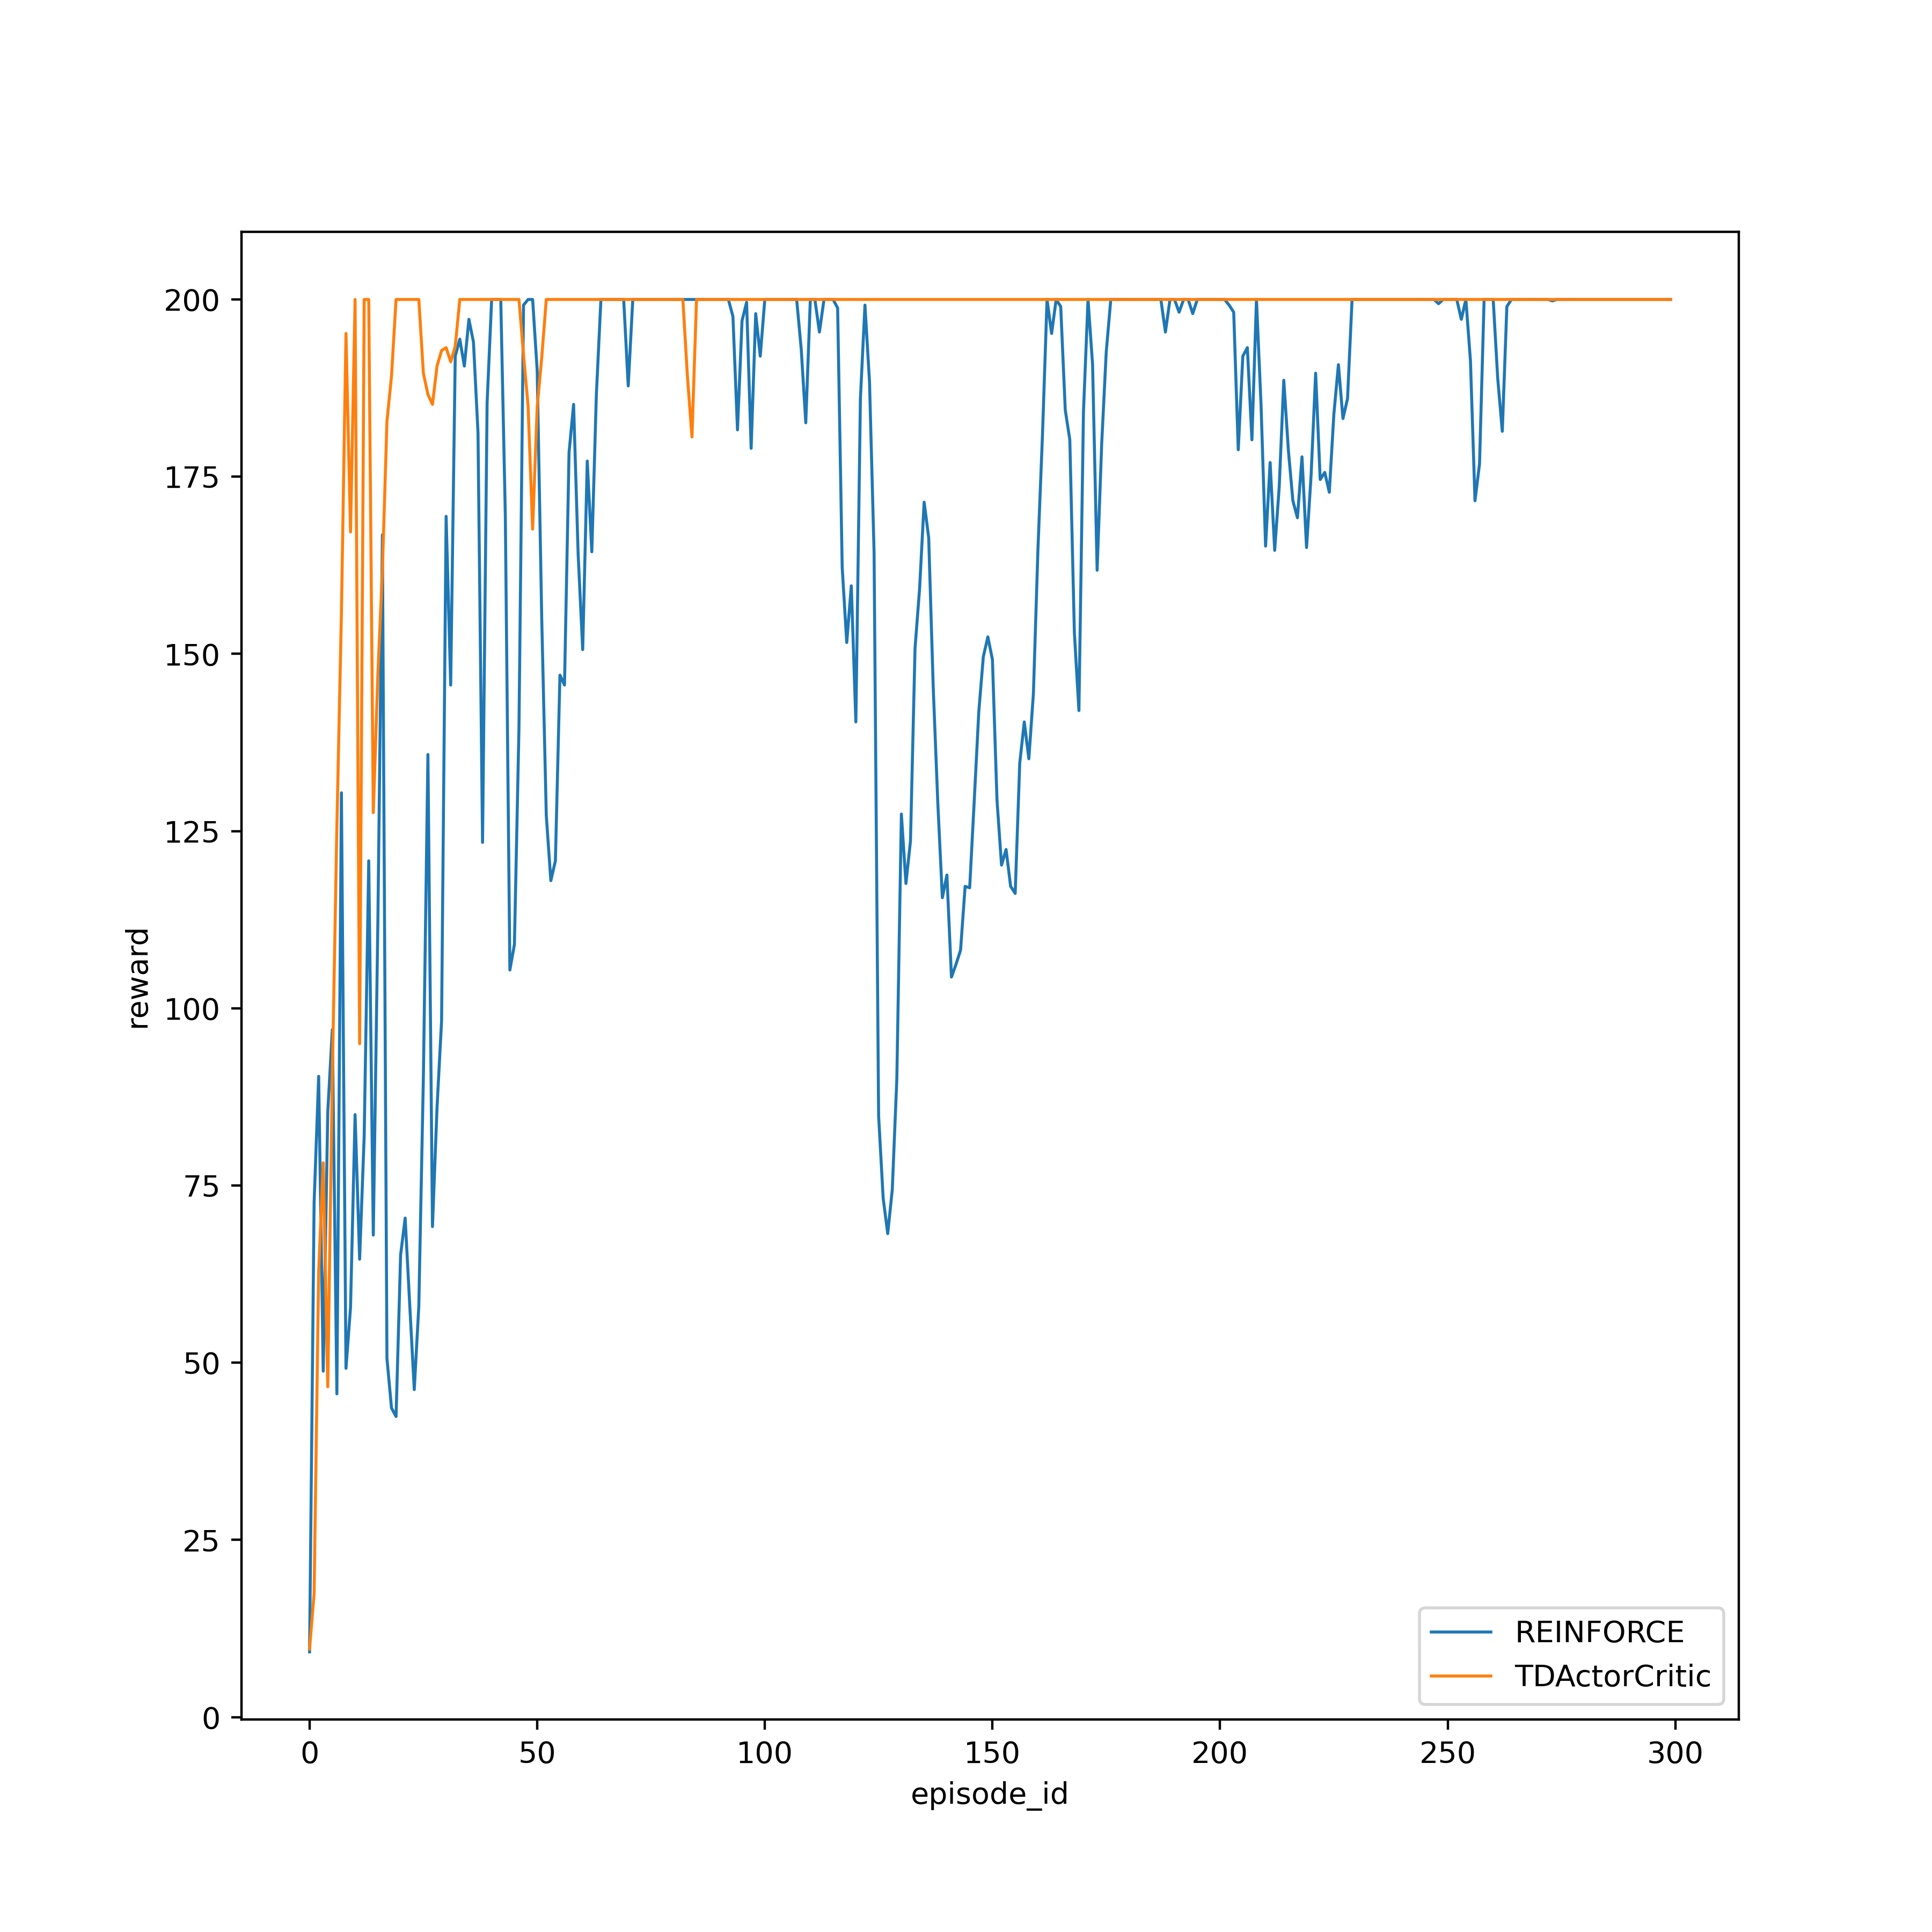
\includegraphics[width=0.40\columnwidth]{./assets/reward (0, v0).png}}
        \subfigure[cartpole-v1, seed=0]{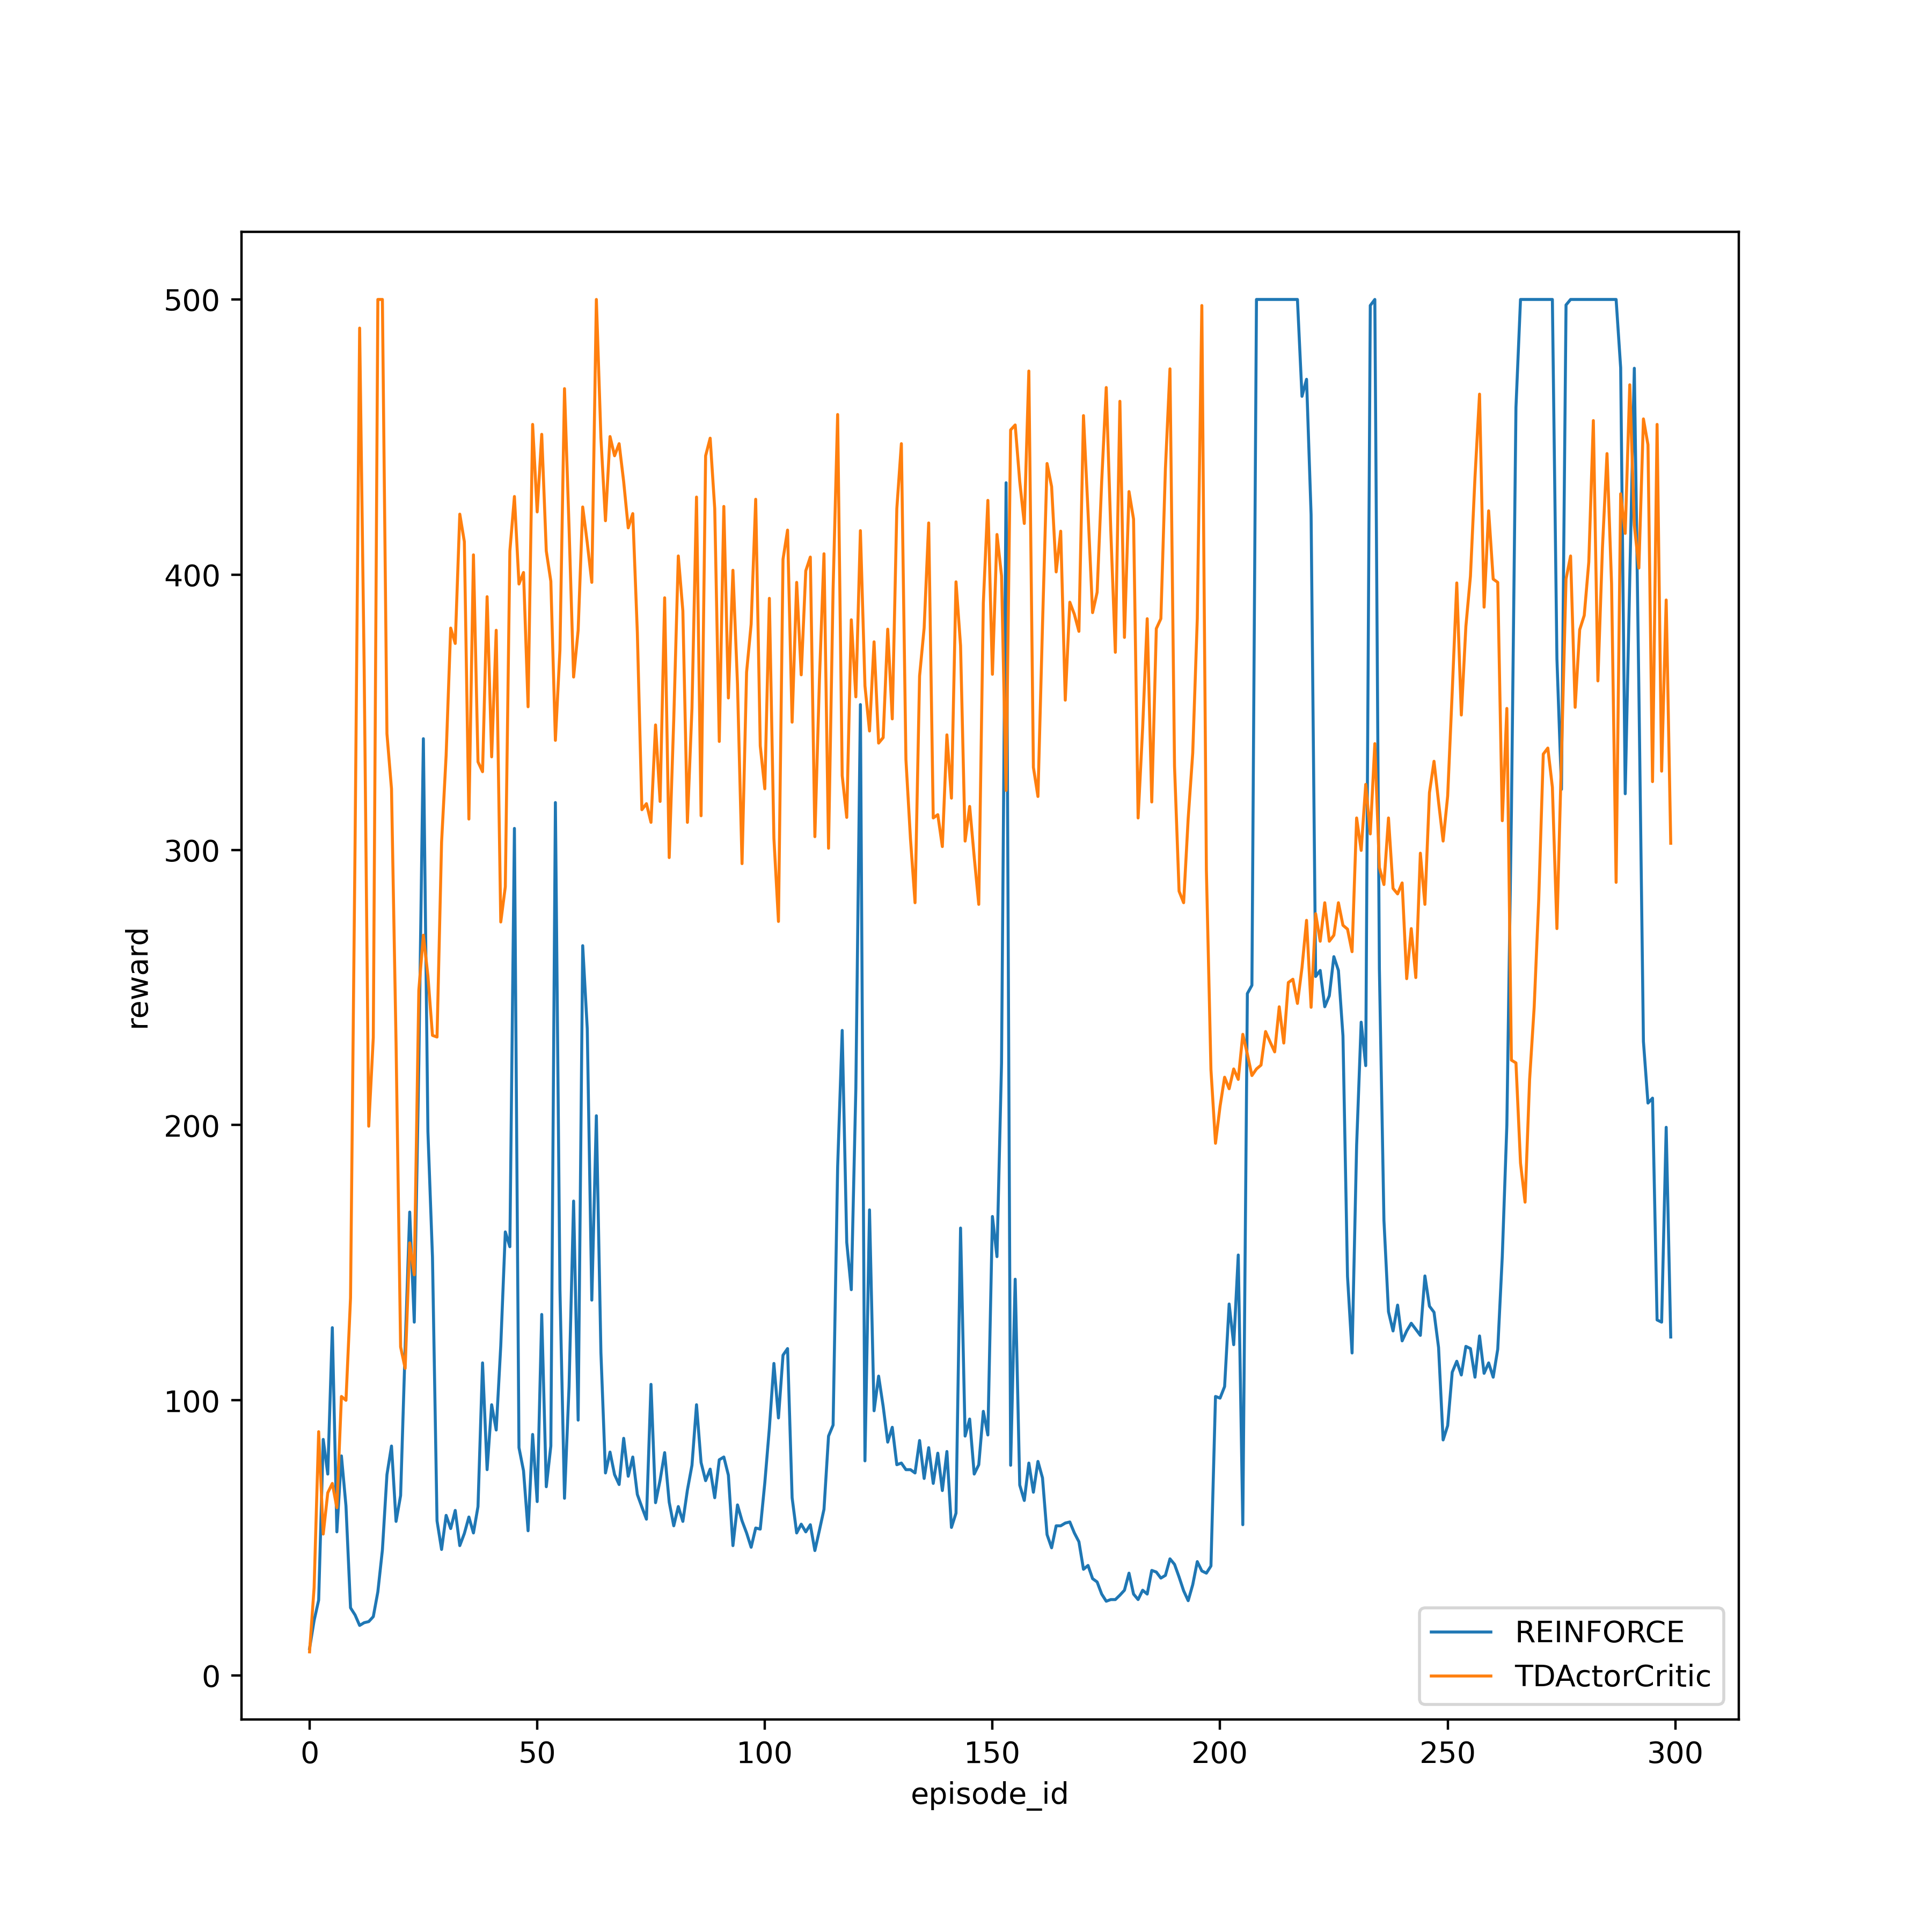
\includegraphics[width=0.40\columnwidth]{./assets/reward (0, v1).png}}
        \subfigure[cartpole-v0, seed=21]{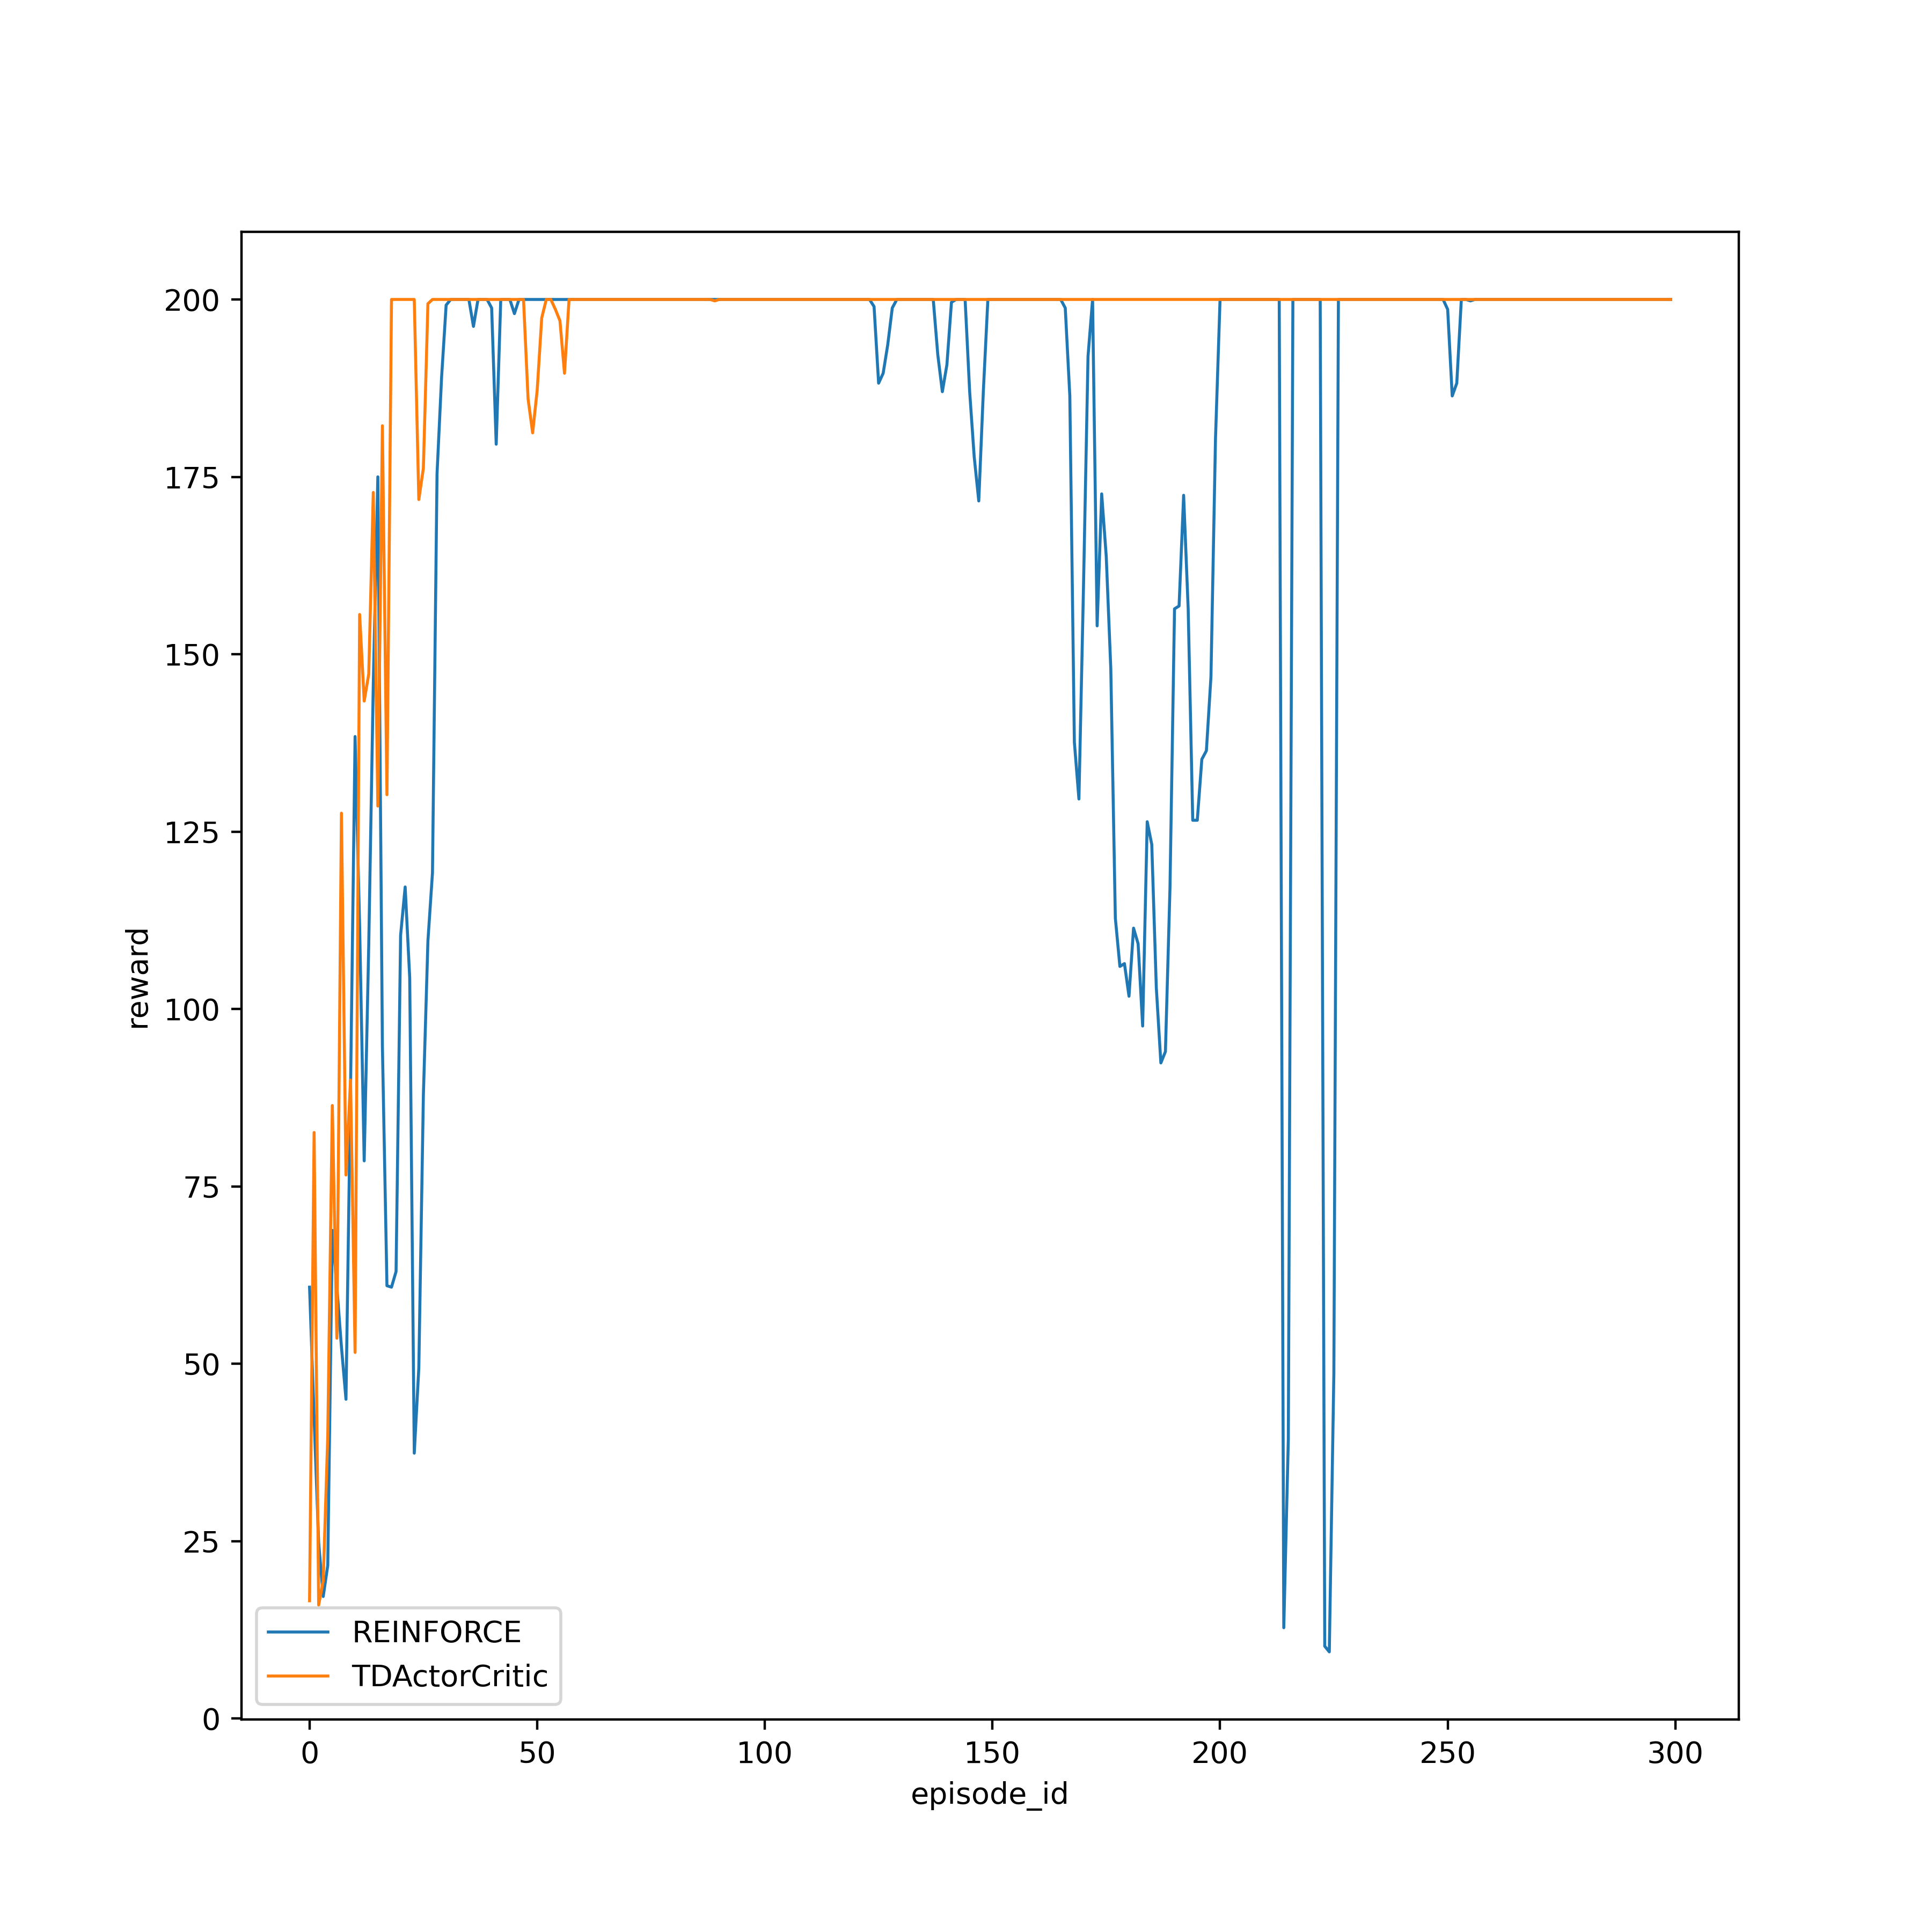
\includegraphics[width=0.40\columnwidth]{./assets/reward (21, v0).png}}
        \subfigure[cartpole-v1, seed=21]{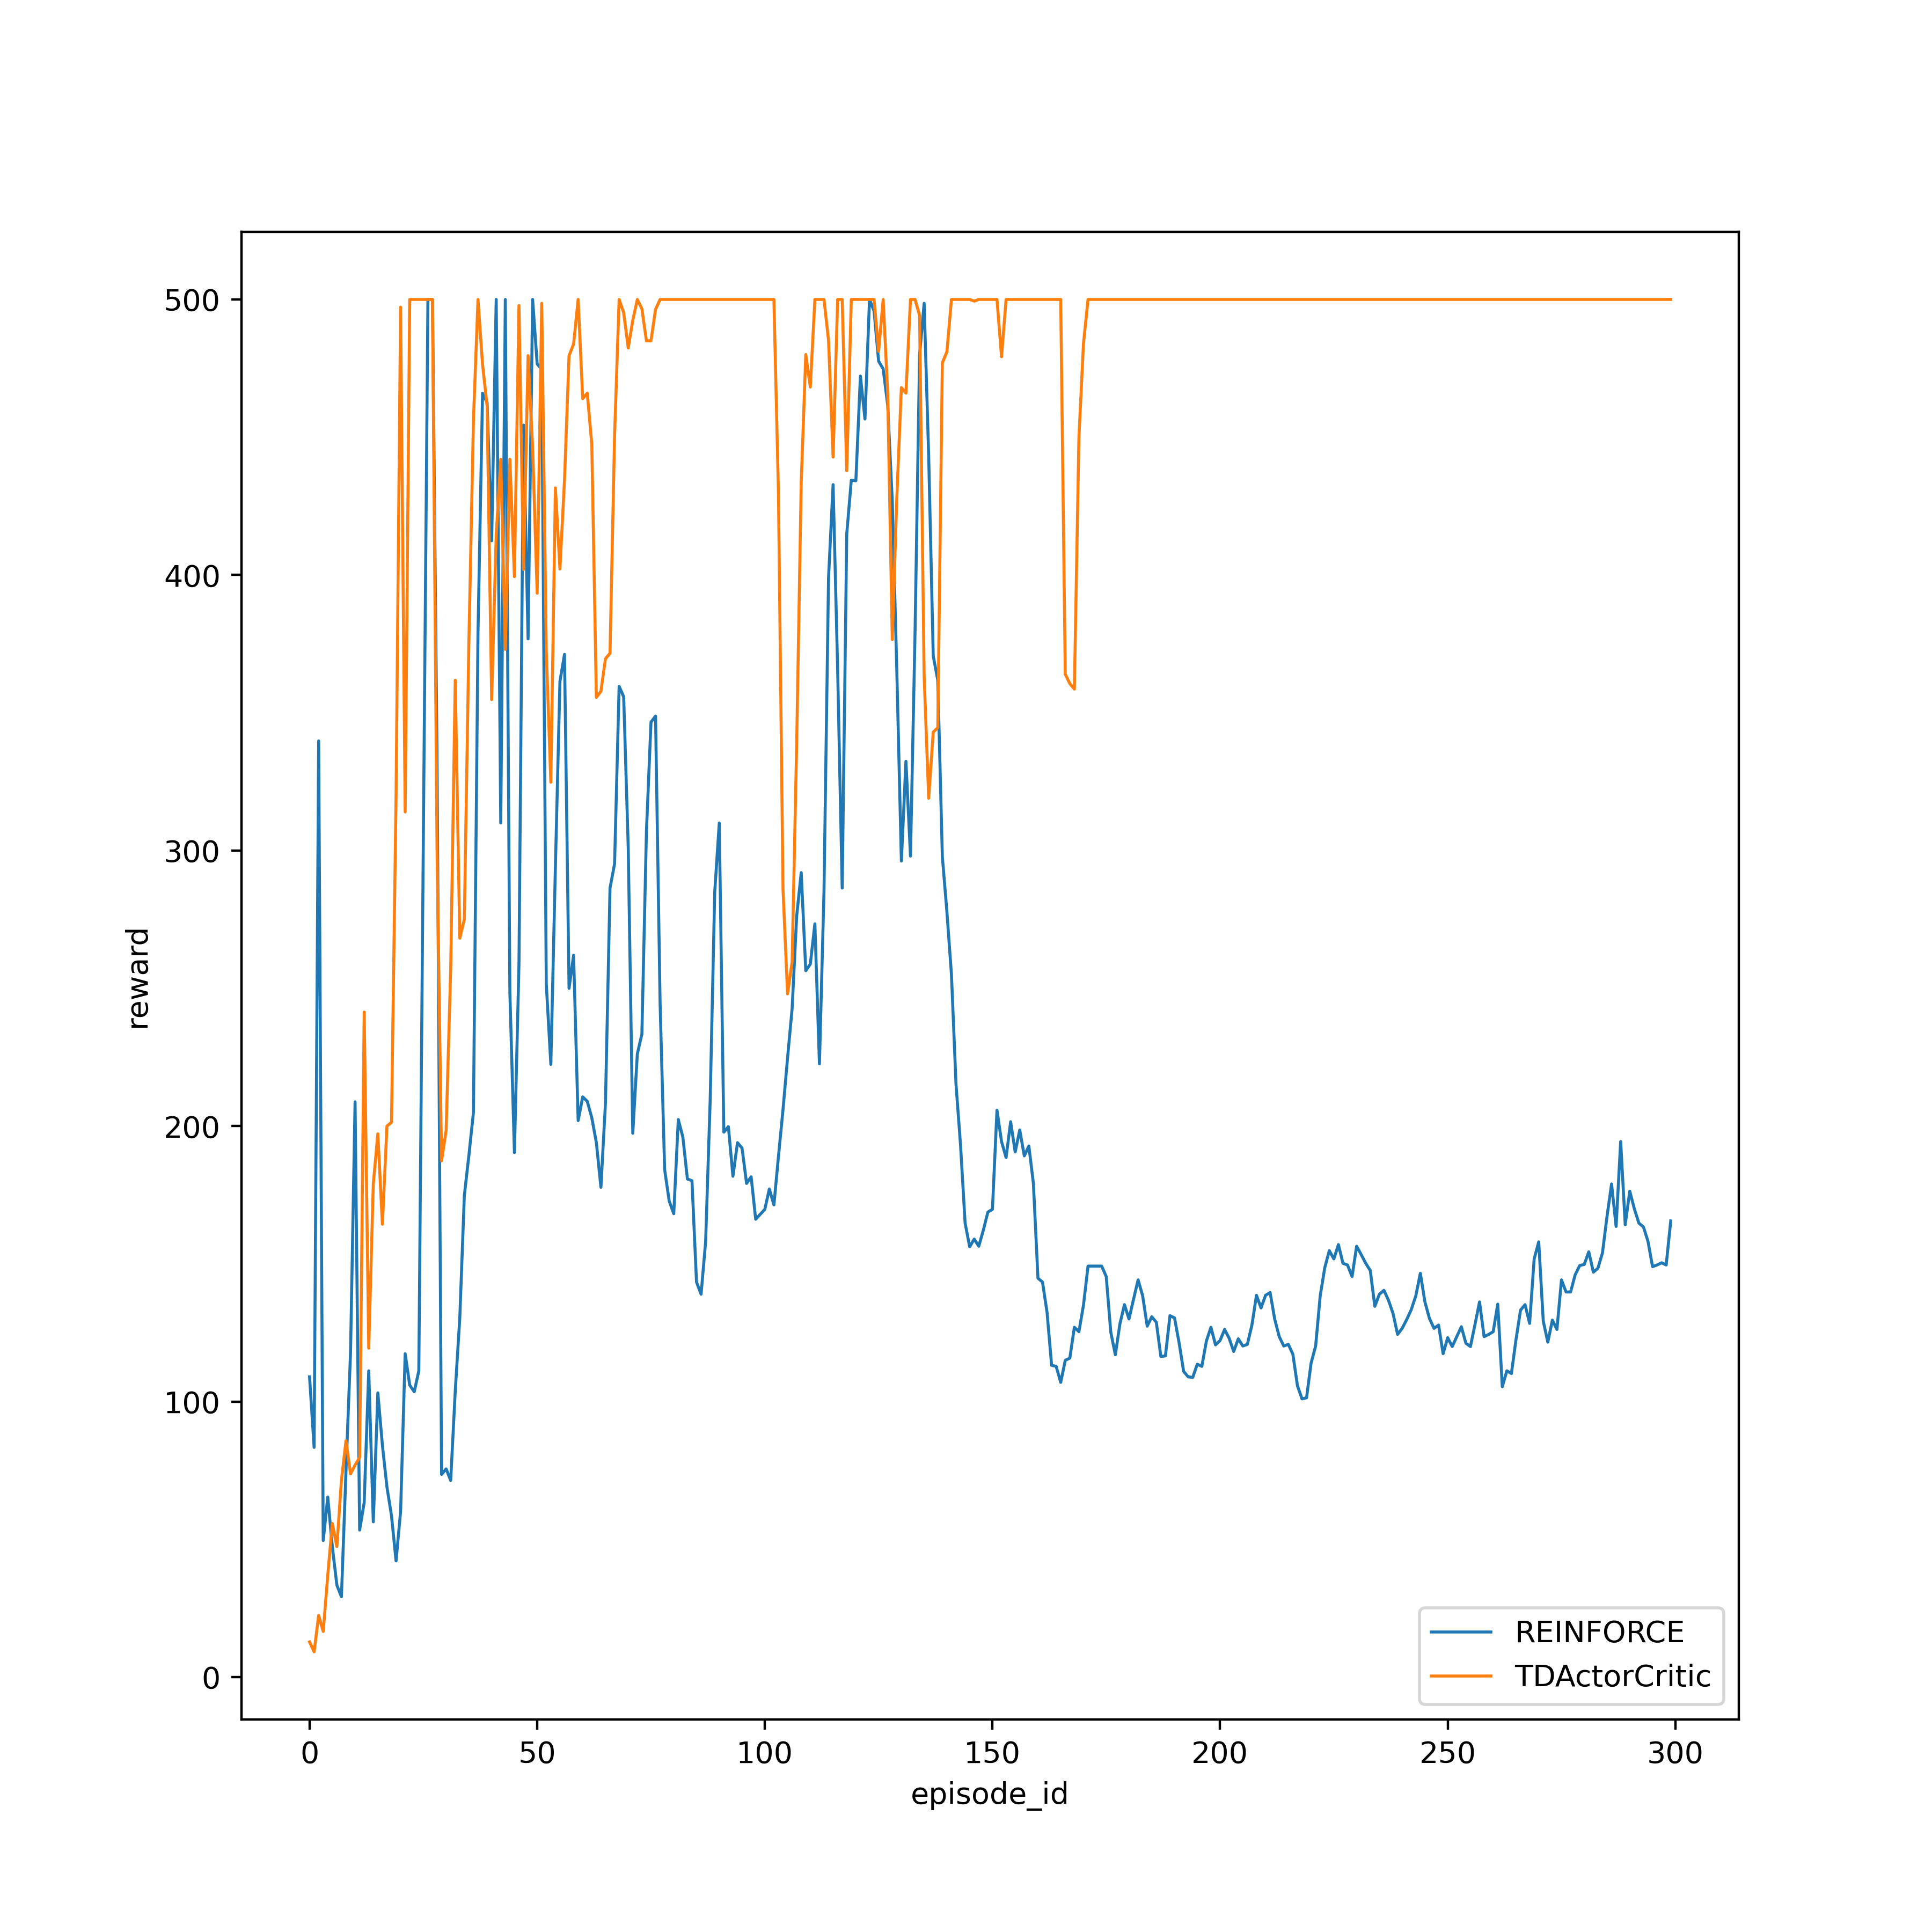
\includegraphics[width=0.40\columnwidth]{./assets/reward (21, v1).png}}
        \subfigure[cartpole-v0, seed=42]{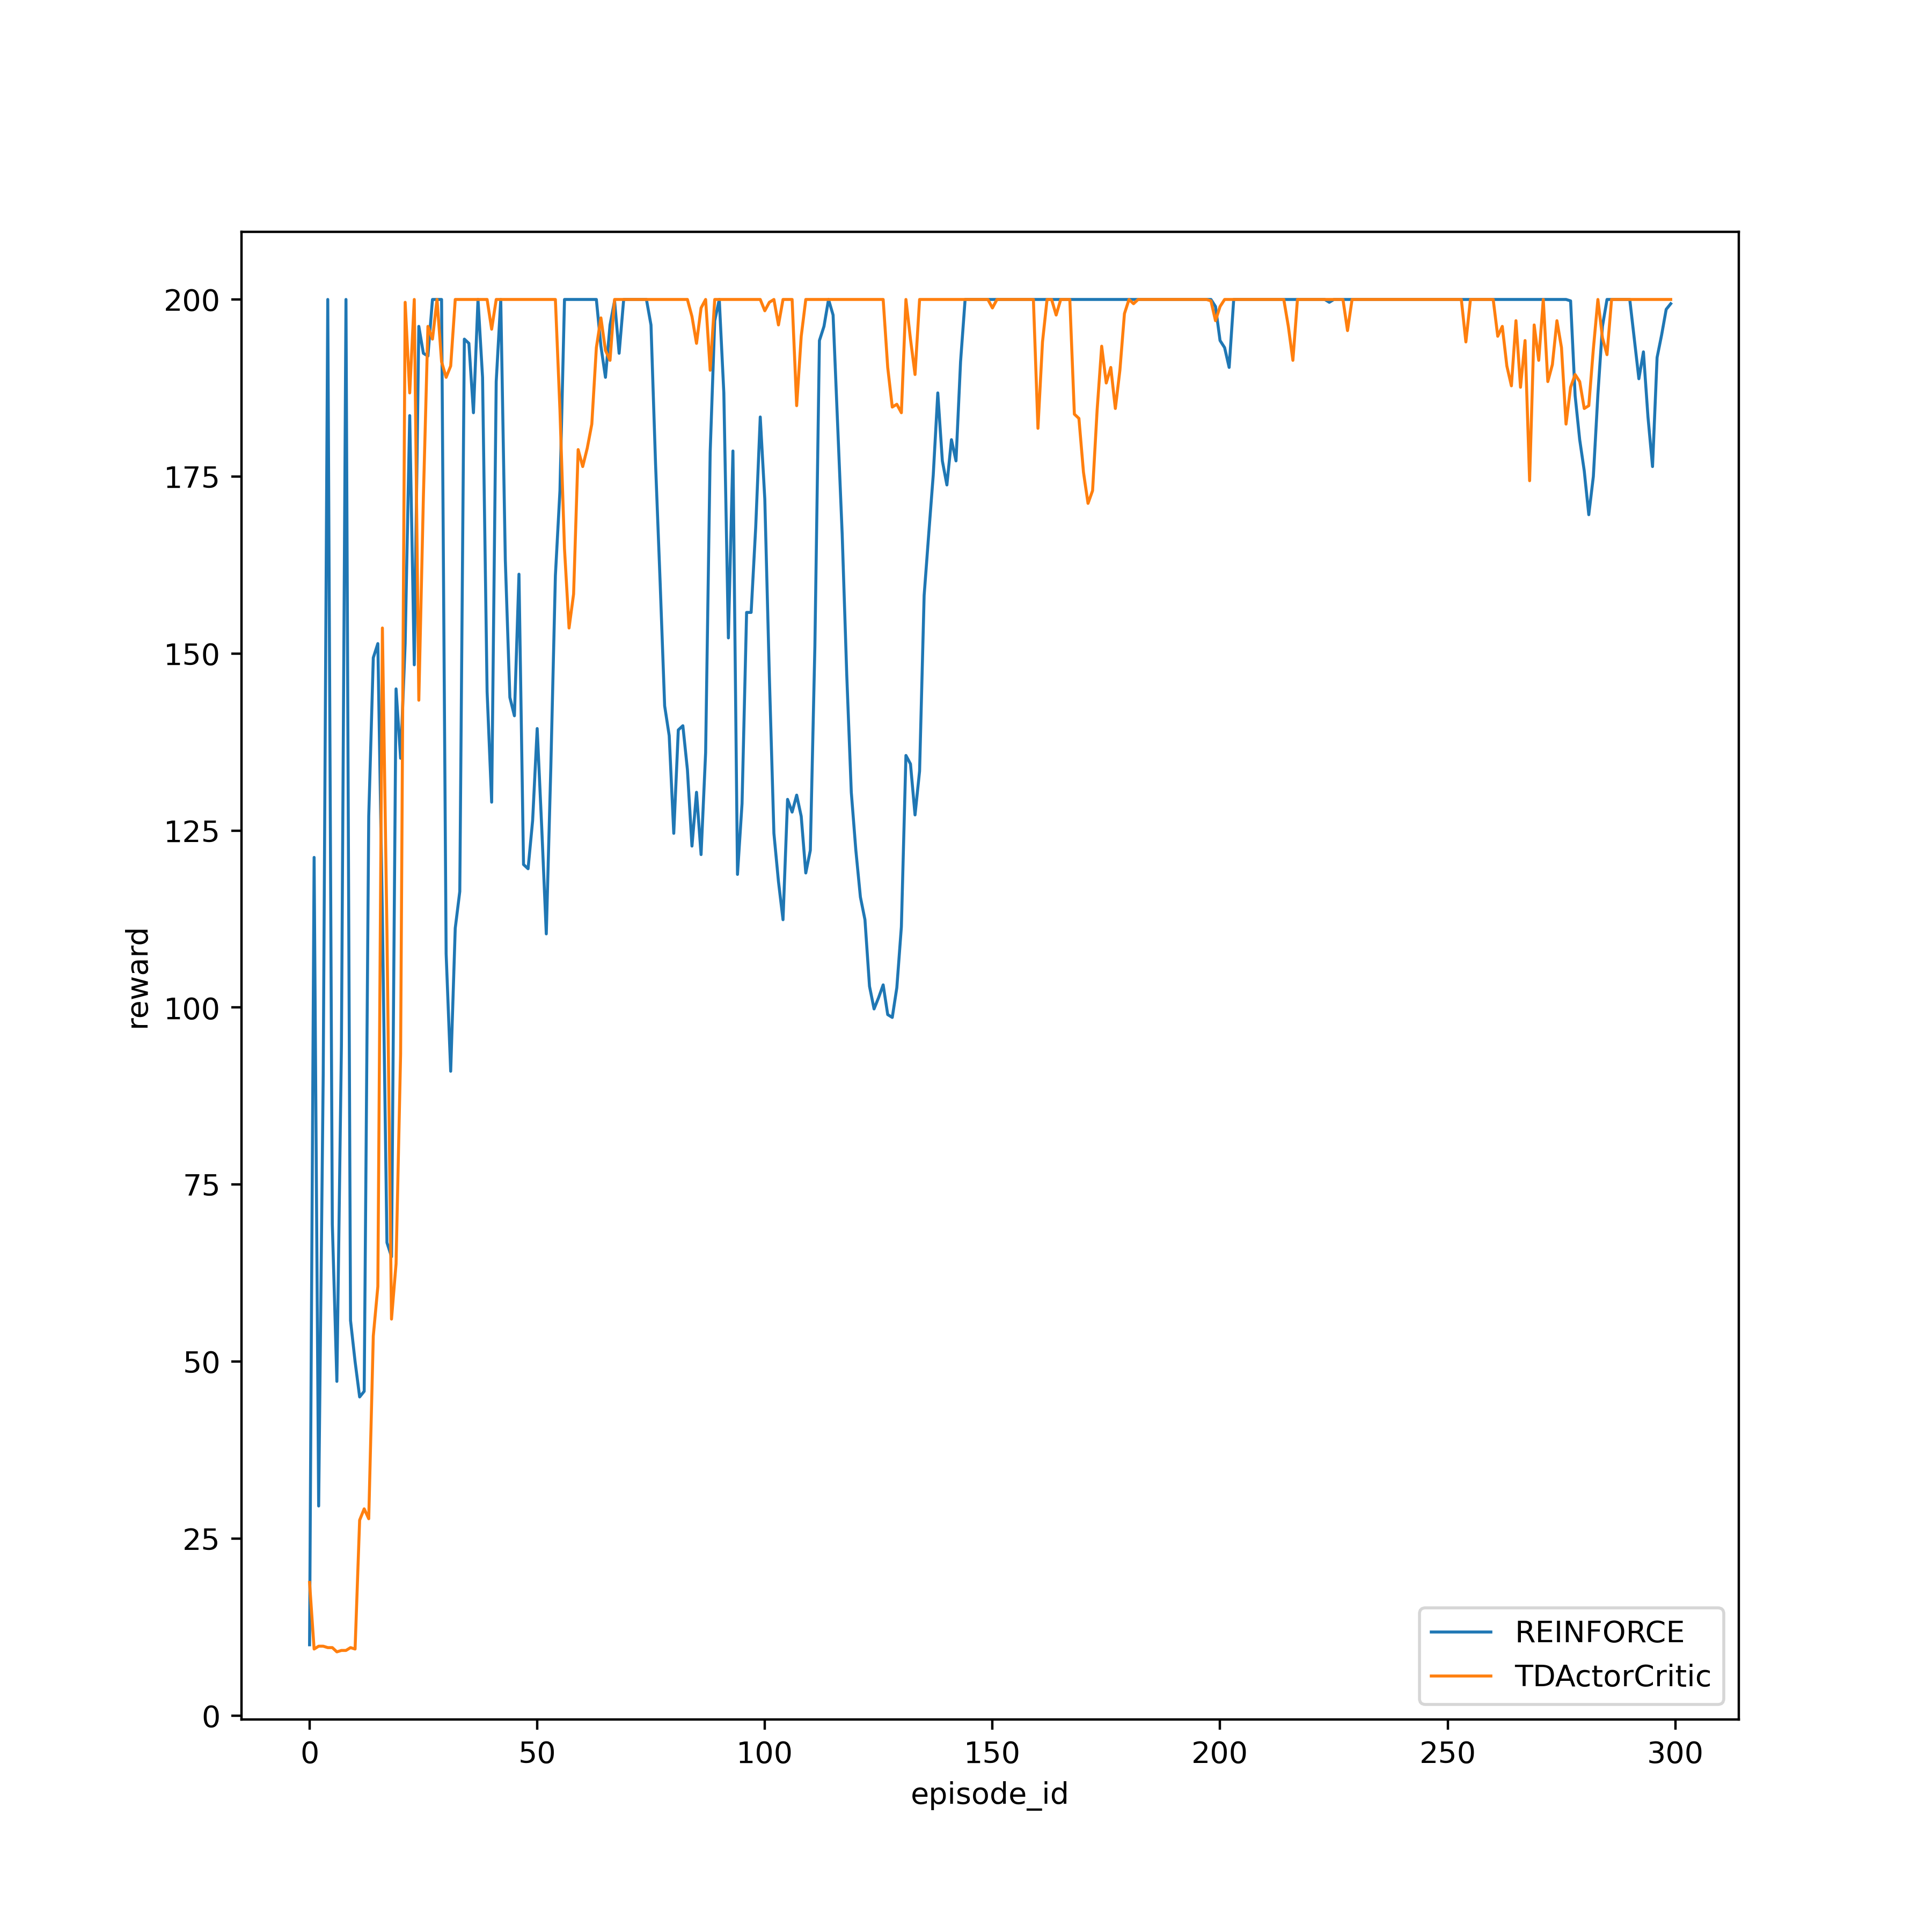
\includegraphics[width=0.40\columnwidth]{./assets/reward (42, v0).png}}
        \subfigure[cartpole-v1, seed=42]{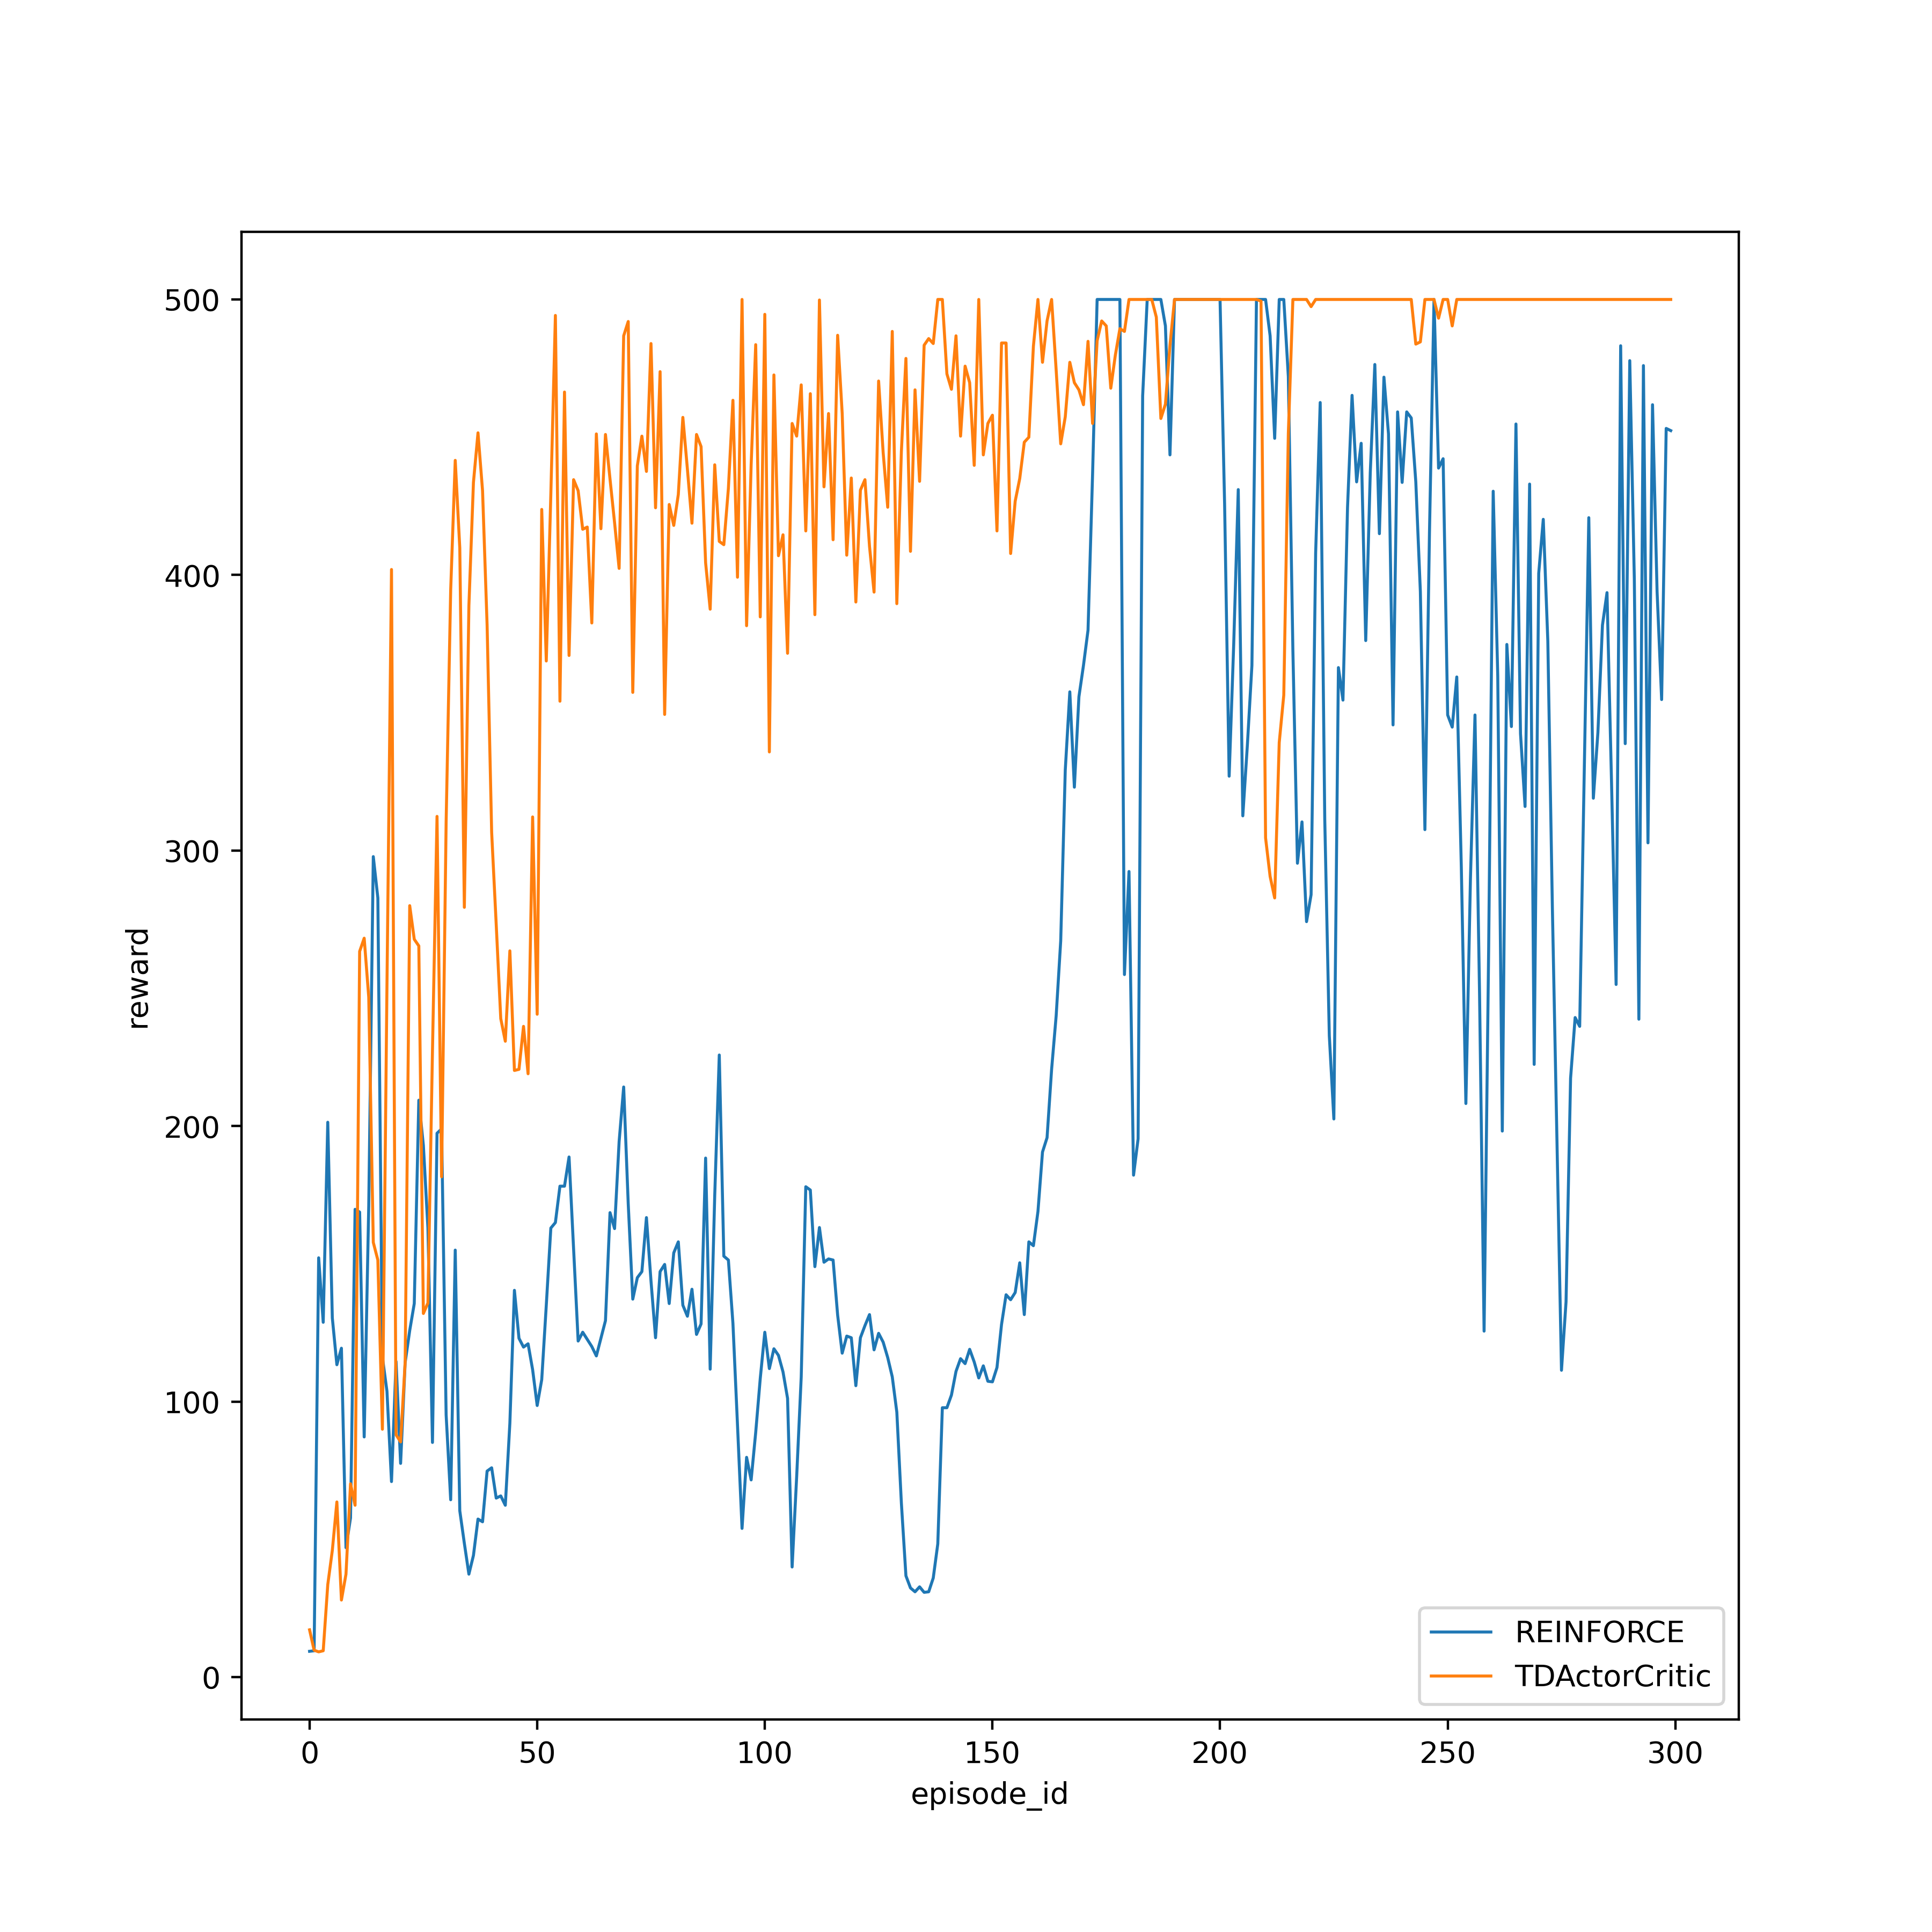
\includegraphics[width=0.40\columnwidth]{./assets/reward (42, v1).png}}
        \caption{两模型在cartpole-v0, cartpole-v1环境训练中的奖励值变化情况}
        \end{figure}

        容易观察到，REINFORCE模型的损失值变化曲线平滑性更差，且在整个训练过程中都存在较为剧烈的抖动现象。
        而TDActorCritic模型的损失值变化曲线收敛较快，且在收敛后抖动很小。因此，可以认为TDActorCritic模型的具有更为稳定的训练性质。

        可以看出，在cartpole-v0环境中，REINFORCE模型和TDActorCritic模型都可以收敛，并取得最大的奖励值200。
        对比而言，REINFORCE模型的收敛速度更慢，且稳定性更差，更容易在训练过程中出现奖励值降低的问题。
        这证明了TDActorCritic模型的收敛效率更高。

        而在cartpole-v1环境中，REINFORCE模型一般不能取得最大的奖励值500，
        而TDActorCritic模型在三次随机试验中的两次都取得了最大的奖励值500，
        结果稍差的一次也取得了450左右的最终奖励。
        基于这一结果，我们认为TDActorCritic模型的能力更强，更有可能学习到较优的策略。

    \end{enumerate}

\end{document}
